% 'Notas de aula não oficiais de MS650 e F620' (c) 2012, 2013 de Raniere Silva
% <ra092767@ime.unicamp.br>
%
% Este trabalho é baseado nos manuscritos das notas de aula do Professor Doutor
% Jayme Vaz Júnior. para as disciplinas MS650, Métodos de Matemática Aplicada
% II, e F620, Métodos Matemáticos da Física II, disponibilizadas em
% http://www.ime.unicamp.br/~vaz/metodos2S12.htm. É permitido a este fazer uso
% deste trabalho para qualquer fim e sem nenhuma restrição.
%
% É permitido fazer uso das criações do espírito presentes neste trabalho
% diretamente relacionadas com os manuscritos das notas de aula do Professor
% Doutor Jayme Vaz Júnior única e exclusivamente para fins educacionais.
%
% Salvo indicação em contrário, este trabalho foi licenciado com a Creative
% Commons Atribuição-CompartilhaIgual 3.0 Não Adaptada. Para ver uma cópia desta
% licença, visite http://creativecommons.org/licenses/by-sa/3.0/.
%
% Este trabalho encontra-se disponível em
% https://github.com/r-gaia-cs/solucoes_ms650_f620.
%
% Este trabalho é distribuído na esperança que possa ser útil, mas SEM NENHUMA
% GARANTIA; sem uma garantia implícita de ADEQUAÇÃO a qualquer MERCADO ou
% APLICAÇÃO EM PARTICULAR.

% O arquivo mestre.

\documentclass[12pt,a4paper,leqno, openright,twoside]{book}
% Filename: paper_size.tex
%
% This code is part of 'Solutions for MS650, Métodos de Matemática Aplicada II, and F620, Métodos Matemáticos da F\'{i}sica II'
% 
% Description: This file corresponds to the paper size output.
% 
% Created: 14.07.12 11:13:03 AM
% Last Change: 22.08.12 08:24:31 AM
% 
% Authors:
% - Raniere Silva (2012): initial version
% 
% Copyright (c) 2012 Raniere Silva <r.gaia.cs@gmail.com>
% 
% This work is licensed under the Creative Commons Attribution-ShareAlike 3.0 Unported License. To view a copy of this license, visit http://creativecommons.org/licenses/by-sa/3.0/ or send a letter to Creative Commons, 444 Castro Street, Suite 900, Mountain View, California, 94041, USA.
%
% This work is distributed in the hope that it will be useful, but WITHOUT ANY WARRANTY; without even the implied warranty of MERCHANTABILITY or FITNESS FOR A PARTICULAR PURPOSE.
%
% Para impressão
\usepackage[top=3cm, bottom=3cm, left=2cm, right=2cm]{geometry}

% Para ereaders (Kindle, Nook, Kobo, ...)
% \usepackage[papersize={160mm,200mm},margin=2mm]{geometry}
% \sloppy

% Para tablets (iPad, GalaxyTab, ...)
% \usepackage[papersize={140mm,190mm},margin=2mm]{geometry}
% \sloppy

% Filename: package.tex
% This code is part of 'LaTeX with Vim'.
% 
% Description: This file correspond to the packages to be used.
% 
% Created: 07.06.12 11:30:10 AM
% Last Change: 26.06.12 11:07:21 PM
% 
% Authors:
% - Raniere Silva, r.gaia.cs@gmail.com
% 
% Copyright (c) 2012, Raniere Silva. All rights reserved.
% 
% This work is licensed under the Creative Commons Attribution-ShareAlike 3.0 Unported License. To view a copy of this license, visit http://creativecommons.org/licenses/by-sa/3.0/ or send a letter to Creative Commons, 444 Castro Street, Suite 900, Mountain View, California, 94041, USA.
%
% This work is distributed in the hope that it will be useful, but WITHOUT ANY WARRANTY; without even the implied warranty of MERCHANTABILITY or FITNESS FOR A PARTICULAR PURPOSE.
%
\usepackage[utf8]{inputenc}
\usepackage[T1]{fontenc} 
% \usepackage[top=3cm,left=2cm,right=2cm,bottom=3cm]{geometry}  % Set in the file.
% \usepackage[brazil]{babel}  % Set in the file.
% \usepackage{indentfirst}  % Set in the file.

% Text
\usepackage{enumerate}
\usepackage{latexsym}
\usepackage{parcolumns}
\usepackage[hyphens]{url}
\usepackage{hyperref}
\usepackage{breakurl}
\usepackage[official]{eurosym}

% Tables
\usepackage{multicol}
\usepackage{multirow}
\usepackage{array}

% Math
\usepackage{amsmath}
\usepackage{amsthm}
\usepackage{amsfonts}
\usepackage{amssymb}

\newtheorem{defi}{Defini\c{c}\~{a}o}
\newtheorem{prop}{Proposi\c{c}\~{a}o}
\newtheorem{teo}{Teorema}
\newtheorem{exem}{Exemplo}
\newtheorem{obs}{Observa\c{c}\~{a}o}

\newcommand{\id}[1]{\, \mathrm{d}#1}

% Index
\usepackage{makeidx}
\makeindex

% Figures
\usepackage{pb-diagram}
\usepackage{graphicx, color}
\usepackage{subfig}
\usepackage{tikz}
\usetikzlibrary{patterns}
\usepackage{epsfig}


\begin{document}
\title{Notas de aula não oficiais de MS650 e F620}
\author{Jayme Vaz (texto) \\ \url{vaz@ime.unicamp.br} \and Raniere Silva
(digitação) \\ \url{ra092767@ime.unicamp.br}}
\maketitle
\thispagestyle{empty}  % Verso da capa.
% Frontmatter
\frontmatter

\tableofcontents

% Mainmatter
\mainmatter

% 'Notas de aula não oficiais de MS650 e F620' (c) 2012, 2013 de Raniere Silva
% <ra092767@ime.unicamp.br>
%
% Este trabalho é baseado nos manuscritos das notas de aula do Professor Doutor
% Jayme Vaz Júnior. para as disciplinas MS650, Métodos de Matemática Aplicada
% II, e F620, Métodos Matemáticos da Física II, disponibilizadas em
% http://www.ime.unicamp.br/~vaz/metodos2S12.htm. É permitido a este fazer uso
% deste trabalho para qualquer fim e sem nenhuma restrição.
%
% É permitido fazer uso das criações do espírito presentes neste trabalho
% diretamente relacionadas com os manuscritos das notas de aula do Professor
% Doutor Jayme Vaz Júnior única e exclusivamente para fins educacionais.
%
% Salvo indicação em contrário, este trabalho foi licenciado com a Creative
% Commons Atribuição-CompartilhaIgual 3.0 Não Adaptada. Para ver uma cópia desta
% licença, visite http://creativecommons.org/licenses/by-sa/3.0/.
%
% Este trabalho encontra-se disponível em
% https://github.com/r-gaia-cs/solucoes_ms650_f620.
%
% Este trabalho é distribuído na esperança que possa ser útil, mas SEM NENHUMA
% GARANTIA; sem uma garantia implícita de ADEQUAÇÃO a qualquer MERCADO ou
% APLICAÇÃO EM PARTICULAR.

% Este arquivo inclui o conteúdo de:
%
% * M2S12-1.pdf
% * M2S12-2.pdf
% * M2S12-3.pdf
% * M2S12-4.pdf
% * M2S12-5.pdf

\chapter{Séries de Fourier}
A série
\begin{dmath*}
  \frac{A_0}{2} + \sum_{n = 1}^\infty \left( A_n \cos\left( n x \right) + B_n
  \sin\left( n x \right) \right)
\end{dmath*}
é chamada uma série trigonométrica.

\begin{defi}
  A série trigonométrica
  \begin{dmath*}
    \frac{a_0}{2} + \sum_{n = 1}^\infty \left( a_n \cos\left( n x \right) + b_n
    \sin\left( n x \right) \right)
  \end{dmath*}
  é a série de Fourier da função $f(x)$ se os coeficientes forem dados por
  \begin{dgroup*}
    \begin{dmath*}
      a_n = \frac{1}{n} \int_{-\pi}^\pi f(x) \cos\left( n x \right) \vi{x}
      \condition{$n = 0, 1, 2, \ldots$}
    \end{dmath*}
    \begin{dmath*}
      b_n = \frac{1}{\pi} \int_{-\pi}^\pi f(x) \sin\left( n x \right) \vi{x}
      \condition{$n = 1, 2, \ldots$}
    \end{dmath*}
  \end{dgroup*}
\end{defi}

Algumas questões:
\begin{enumerate}
  \item a série converge?
  \item qual o intervalo de convergência?
  \item qual o tipo de convergência?
    \begin{exem}
      Para a convergência uniforme temos que $\forall \epsilon > 0, \exists
      n > 0$ tal que $| \delta_m(x) - \delta_n(x)| < \epsilon$ sempre que $m, n
      > N, \forall x \in I$ (onde $\delta_n(x) = \sum_{k = 1}^\nu \mu_k(x)$).
    \end{exem}
  \item quais funções $f(x)$ são representáveis por essa série? Condições sobre
    $f(x)$?
\end{enumerate}

Um fato notável é que as condições para representar uma função por uma série de
Fourier são menos restritivas do que para séries de potências.

\begin{obs}
  Temos que $\left\{ \cos\left( n x \right), \sin\left( n x \right) \right\}$
  são funções periódicas com $T = 2\pi$ e portanto $f(x)$ é uma função
  periódica, i.e., $f(x + 2\pi) = f(x)$.
\end{obs}

\begin{exem} \label{exem:fourier:x^2}
  Para $f(x) = x^2$ temos que
  \begin{dgroup*}
    \begin{dmath*}
      a_0 = \frac{1}{\pi} \int_{-\pi}^\pi x^2 \vi{x} = \frac{1}{\pi} \left.
      \frac{x^3}{3} \right|_{-\pi}^\pi = \frac{2 \pi^2}{3},
    \end{dmath*}
    \begin{dmath*}
      a_n = \frac{1}{n} \int_{\pi}^\pi x^2 \cos\left( n x \right) \vi{x}
      = \frac{1}{\pi} \left[ \underbrace{\left. \frac{x^2 \sin\left( n x
      \right)}{n} \right|_{-\pi}^\pi}_{= 0} - \frac{1}{n} \int_{-\pi}^\pi 2 x
      \sin\left( n x \right) \vi{x} \right]
      = \frac{-1}{n \pi} \left[ \left. \frac{-2 x \cos\left( n x \right)}{n}
      \right|_{-\pi}^\pi + \frac{1}{n} \int_{-\pi}^\pi 2 \cos\left( n x \right)
      \vi{x} \right]
      = \frac{-1}{n \pi} \left[ \frac{-2 \pi \cos\left( n \pi) \right)}{n} +
      \frac{2 (-\pi) \cos(n) (-\pi)}{n} + \frac{2}{n} \underbrace{\left.
      \frac{\sin\left( n x \right)}{n} \right|_{-\pi}^\pi}_{= 0} \right]
      = \frac{-1}{n \pi} \left[ \frac{- 4 \pi}{n} \cos\left( n \pi \right)
      \right]
      = \frac{4}{n^2} (-1)^n,
    \end{dmath*}
    \begin{dmath*}
      b_n = \frac{1}{n} \int_{-\pi}^\pi x^2 \sin\left( n x \right) \vi{x}
      = \frac{1}{\pi} \left[ \left. \frac{- x^2 \cos\left( n x \right)}{n}
      \right|_{-\pi}^\pi + \frac{1}{n} \int_{-\pi}^\pi 2 x \cos\left( n x
      \right) \vi{x} \right]
      = \frac{1}{n} \left[ \frac{-\pi^2 \cos\left( n \pi \right)}{n} + \frac{\pi
      \cos\left( n (-\pi) \right)}{n} + \frac{1}{n} \int_{-\pi}^\pi 2 x
      \cos\left( n x \right) \vi{x} \right]
      = \frac{1}{n} \left[ \frac{1}{n} \left[ \underbrace{\left. \frac{2 x
      \sin\left( n x \right)}{n} \right|_{-\pi}^\pi}_{= 0} - \frac{1}{n}
      \underbrace{\int_{-\pi}^\pi 2 \sin\left( n x \right) \vi{x}}_{= 0} \right]
      \right]
      = 0,
    \end{dmath*}
  \end{dgroup*}
  onde $n > 0$.

  Logo,
  \begin{dmath*}
    x^2 = \frac{\pi^2}{3} + \sum_{n = 1}^\infty \frac{4 (-1)^n}{n^2} \cos\left(
    n x \right).
  \end{dmath*}
\end{exem}

\begin{obs}
  Essa série representa $f(x) = x^2$ para $-\pi \leq x \leq \pi$. Para os demais
  pontos trata-se da extensão periódica de $f(x) = x^2$, $-\pi \leq x \leq \pi$.
\end{obs}

\begin{figure}[!htb]
  \centering
  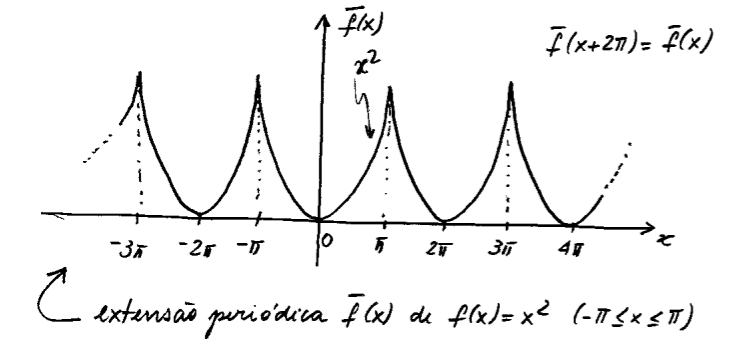
\includegraphics[width=0.8\textwidth]{figuras/01-0}
  \caption{Gráfico da série de Fourier para $f(x) = x^2$.}
  \label{fig:serie_fourier_grafico01}
\end{figure}

\begin{exem}
  Para
  \begin{dmath*}
    f(x) = \begin{cases}
      -1, & x < 0, \\
      +1, & x \geq 0.
    \end{cases}
  \end{dmath*}
  temos que
  \begin{dgroup*}
    \begin{dmath*}
      a_0 = \frac{1}{\pi} \int_{-\pi}^\pi f(x) \vi{x}
      = \frac{1}{\pi} \left[ -\int_\pi^0 \vi{x} + \int_0^\pi \vi{x} \right]
      = 0,
    \end{dmath*}
    \begin{dmath*}
      a_n = \frac{1}{\pi} \int_{-\pi}^\pi f(x) \cos\left( n x \right) \vi{x}
      = \frac{1}{n} \left[ -\int_{-\pi}^0 \cos\left( n x \right) \vi{x} +
      \int_0^\pi \cos\left( n x \right) \vi{x} \right]
      = 0,
    \end{dmath*}
    \begin{dmath*}
      b_n = \frac{1}{\pi} \int_{-\pi}^\pi f(x) \sin\left( n x \right) \vi{x}
      = \frac{1}{\pi} \left[ -\int_{-\pi}^0 \sin\left( n x \right) \vi{x} +
      \int_0^\pi \sin\left( n x \right) \vi{x} \right]
      = \frac{2}{\pi} \int_0^\pi \sin\left( n x \right) \vi{x}
      = \left. \frac{-2 \cos\left( n x \right)}{n \pi} \right|_0^\pi
      = \frac{-2}{n \pi} \left[ (-1)^n - 1 \right]
      = \begin{cases}
        0, & n \text{ é par}, \\
        4 / \left( n \pi \right), & n \text{ é ímpar}.
      \end{cases}
    \end{dmath*}
  \end{dgroup*}

  Logo,
  \begin{dmath*}
    f(x) = \sum_{n = 1}^\infty b_n \sin\left( n x \right)
    = \sum_{k = 1}^\infty b_{k + 1} \sin\left( (2k + 1) x \right)
    = \sum_{k = 0}^\infty \frac{4}{\left( 2k + 1 \right) \pi} \sin\left( (2k + 1) x \right).
  \end{dmath*}
\end{exem}

\begin{figure}[!htb]
  \centering
  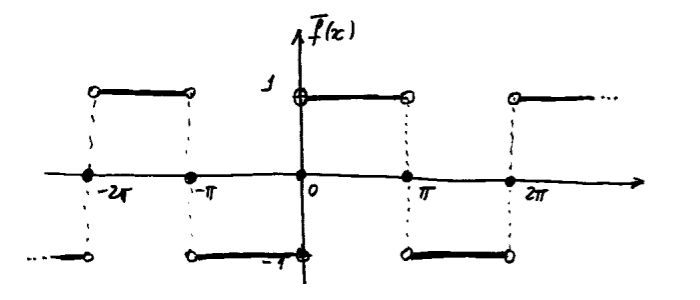
\includegraphics[width=0.8\textwidth]{figuras/01-1}
    % TODO Arrumar o comando \caption abaixo.
  \caption{Gráfico da série de Fourier para }
  \label{fig:serie_fourier_grafico02}
\end{figure}

Pela Figura~\ref{fig:serie_fourier_grafico02} que
\begin{dmath*}
  \bar{f}(x) = \begin{cases}
    1, & 0 < x < \pi, \\
    0, & x = 0, \pi, -\pi, \\
    -1, & -\pi < x < 0.
  \end{cases}
\end{dmath*}
e
\begin{dmath*}
  \bar{f}(x + 2 \pi) = \bar{f}(x).
\end{dmath*}

\begin{obs}
  $\bar{f}(0) \neq f(0)$, o que é característico do comportamento da série de
  Fourier em uma descontinuidade. Note que
  \begin{dmath*}
    \bar{f}(0) = \frac{1}{2} \left[ \lim_{x \to 0^+} f(x) + \lim_{x \to 0^-}
    f(x) \right]
  \end{dmath*}
  nesse caso (que se mostrará verdade no caso geral!).
\end{obs}

\begin{defi}
  Seja $\mathcal{L}^2[a, b]$ o conjunto das funções de quadrado integrável em $a
  \leq x \leq b$. Dizemos que $f(x)$ e $g(x)$ são ortogonais nesse intervalo se
  \begin{dmath*}
    \int_a^b f(x) g(x) \vi{x} = 0.
  \end{dmath*}
\end{defi}

\begin{obs}
  Lembrando que
  \begin{dmath*}
    0 \leq \left( f - g \right)^2 = f^2 + g^2 - 2 f g,
  \end{dmath*}
  ou seja,
  \begin{dmath*}
    2 f g \leq f^2 + g^2,
  \end{dmath*}
  concluímos que se $f, g \in \mathcal{L}^2[a, b]$, então existe $\int_a^b f(x)
  g(x) \vi{x}$. Além disso,
  \begin{dmath*}
    \left( f + g \right)^2 = f^2 + g^2 + 2 f g \leq 2 \left( f^2 + g^2 \right),
  \end{dmath*}
  o que garante que $f + g \in \mathcal{L}^2[a, b]$. Como $\mathcal{L}^2[a, b]$
  é um espaço vetorial, podemos pensar nessa integral como o produto escalar
  $<f, g>$ de $f, g \in \mathcal{L}^2[a, b]$:
  \begin{dmath*}
    \langle f, g \rangle = \int_a^b f(x) g(x) \vi{x}.
  \end{dmath*}
\end{obs}

\begin{prop}
  O conjunto $\left\{ 1, \cos\left( n x \right), \sin\left( n x \right)
  \right\}$ ($n = 1, 2, \ldots$) é ortogonal em $[-\pi, \pi]$.
\end{prop}
\begin{proof}
  Devemos mostrar que
  \begin{dgroup}
    \begin{dmath}[label={eq:serie_fourier_ort01}]
      \int_{-\pi}^\pi 1 \cos\left( n x \right) \vi{x} = \int_{-\pi}^\pi 1 \sin
      \left( n x \right) \vi{x} = 0,
    \end{dmath}
    \begin{dmath}[label={eq:serie_fourier_ort02}]
      \int_{-\pi}^\pi \cos\left( n x \right) \cos\left( m x \right) \vi{x} =
      \int_{-\pi}^\pi \sin\left( n x \right) \sin\left( m x \right) \vi{x} = 0
      \condition{$n \neq m$,}
    \end{dmath}
    \begin{dmath}[label={eq:serie_fourier_ort03}]
      \int_{-\pi}^\pi \cos\left( n x \right) \sin\left( m x \right) \vi{x} = 0.
    \end{dmath}
  \end{dgroup}
  As integrais \eqref{eq:serie_fourier_ort01} são triviais. Quanto a
  \eqref{eq:serie_fourier_ort02} e \eqref{eq:serie_fourier_ort03}, elas são
  calculadas de forma análoga, de modo que faremos explicitamente apenas uma
  delas. Usando a identidade
  \begin{dmath*}
    \cos\left( n x \right) \cos\left( m x \right) = \frac{1}{2} \cos\left( (n -
    m) x \right) + \frac{1}{2} \cos\left( (n + m) x \right)
  \end{dmath*}
  segue, para $n \neq m$, que
  \begin{dmath*}
    \int_{-\pi}^\pi \cos\left( n x \right) \cos\left( m x \right) \vi{x} =
    \frac{1}{2} \left. \frac{\sin\left( (n - m) x \right)}{n - m}
    \right|_{-\pi}^\pi + \frac{1}{2} \left. \frac{\sin\left( (n + m) x
    \right)}{n - m} \right|_{-\pi}^\pi = 0
  \end{dmath*}
  pois $\sin\left( k \pi \right) = 0$ para $k$ inteiro.

  Não custa chamar a atenção para o fato que \eqref{eq:serie_fourier_ort03} vale
  para quaisquer $n$ e $m$, enquanto \eqref{eq:serie_fourier_ort02} vale para $n
  \neq m$. Quando $n = m$, para \eqref{eq:serie_fourier_ort02} temos
  \begin{dmath*}
    \int_{-\pi}^\pi \cos^2\left( n x \right) \vi{x} = \int_{-\pi}^\pi
    \sin^2\left( n x \right) \vi{x} = \pi.
  \end{dmath*}
\end{proof}

\begin{teo}
  Se uma série trigonométrica converge uniformemente para a função $f(x)$ em
  $-\pi \leq x \leq \pi$, então ela é a série de Fourier de $f(x)$.
\end{teo}
\begin{proof}
  Se
  \begin{dmath*}
    f(x) = \frac{A_0}{2} + \sum_{n = 1}^\infty \left( A_n \cos\left( n x \right)
    + B_n \sin\left( n x \right) \right)
  \end{dmath*}
  converge uniformemente, o mesmo acontecerá com a série multiplicada por
  $\cos\left( m x \right)$ ou $\sin\left( m x \right)$. Como uma série
  uniformemente convergente pode ser integrada termo a termo, temos, por exemplo
  \begin{dmath*}
      \int_{-\pi}^\pi f(x) \cos\left( m x \right) \vi{x} = \frac{A_0}{2}
      \underbrace{\int_{-\pi}^\pi \cos\left( m x \right) \vi{x}}_{= 0} + \sum_{n
      = 1}^\infty \left( A_n \underbrace{\int_{-\pi}^\pi \cos\left( n x \right)
      \cos\left( m x \right) \vi{x}}_{= 0 (n \neq m)} + B_n
      \underbrace{\int_{-\pi}^\pi \sin\left( n x \right) \cos\left( m x \right)
      \vi{x}}_{= 0} \right)
  \end{dmath*}
  onde usamos a proposição anterior, de modo que
  \begin{dmath*}
    \int_{-\pi}^\pi f(x) \cos\left( m x \right) \vi{x} = A_m \int_{-\pi}^\pi
    \cos^2\left( m x \right) \vi{x} = \pi A_m,
  \end{dmath*}
  ou seja, $A_m$ é um coeficiente de Fourier. Procedendo de forma análogo,
  veremos que o mesmo acontece com $A_0$ e $B_m$, de modo que se trata de uma
  série de Fourier.
\end{proof}

\section{Mudança de intervalo}
Vamos agora, ao invés de $T = 2 \pi$, considerar um período $T = 2 L$. Para
isso, na série de Fourier
\begin{dmath*}
  f(x') = \frac{a_0}{2} + \sum_{n = 1}^\infty \left( a_n \cos\left( n x' \right)
  + b_n \sin\left( n x' \right) \right),
\end{dmath*}
vamos fazer a mudança de variável
\begin{dmath*}
  x' = \frac{\pi}{L} x.
\end{dmath*}
Assim, para $f(x') = f(\pi x / L) = f(x)$, temos
\begin{dmath*}
  F(x) = \frac{a_0}{2} + \sum_{n = 1}^\infty \left( a_n \cos\left( \frac{n \pi
  x}{L} \right) + b_n \sin\left( \frac{n \pi x}{L} \right) \right),
\end{dmath*}
com
\begin{dmath*}
  a_n = \frac{1}{\pi} \int_{-\pi}^\pi f(x') \cos\left( n x' \right) \vi{x'} =
  \frac{1}{\pi} \int_{-L}^L \frac{\pi}{L} f\left( \frac{\pi}{L} x \right)
  \cos\left( \frac{n \pi x}{L} \right) \vi{x},
\end{dmath*}
ou seja,
\begin{dmath*}
  a_n = \frac{1}{L} \int_{-L}^L F(x) \cos\left( \frac{n \pi x}{L} \right)
  \vi{x} \condition{$ n = 1, 2, \ldots$}
\end{dmath*}
e da mesma forma
\begin{dmath*}
  b_n = \frac{1}{L} \int_{-L}^L F(x) \sin\left( \frac{n \pi x}{L} \right)
  \vi{x} \condition{$n = 1, 2, \ldots$}
\end{dmath*}

\begin{exem}
  Para $f(x) = x^2, - 2 \pi \leq x \leq 2 \pi$ temos, usando $L = 2 \pi$
  (portanto período $T = 4\pi$), encontramos que
  \begin{dmath*}
    x^2 = \frac{4 \pi^2}{3} + \sum_{n = 1}^\infty \frac{16 (-1)^n}{n^2}
    \cos\left( \frac{n x}{2} \right).
  \end{dmath*}
\end{exem}

\section{Forma complexa}
Temos que $\exp(i x) = \cos(x) + i \sin(x)$ e portanto
\begin{dgroup*}
  \begin{dmath*}
    \cos\left( \frac{n \pi x}{L} \right) = \frac{1}{2} \left( \exp\left( i
    \frac{n \pi x}{L} \right) + \exp\left( -i \frac{n \pi x}{L} \right) \right),
  \end{dmath*}
  \begin{dmath*}
    \sin\left( \frac{n \pi x}{L} \right) = \frac{1}{2 i} \left( \exp\left( i
    \frac{n \pi x}{L} \right) - \exp\left( -i \frac{n \pi x}{L} \right) \right).
  \end{dmath*}
\end{dgroup*}
Logo,
\begin{dmath*}
  f(x) = \frac{a_0}{2} + \sum_{n = 1}^\infty \left[ \frac{a_n}{2} \exp\left( i
  \frac{n \pi x}{L} \right) + \frac{a_n}{2} \exp\left( -i \frac{n \pi x}{L}
  \right) - \frac{b_n i}{2} \exp\left( i \frac{n \pi x}{L} \right) + \frac{b_n
  i}{2} \exp\left( -i \frac{n \pi x}{L} \right) \right]
  = \frac{a_0}{2} + \sum_{n = 1}^\infty \underbrace{\left( \frac{a_n - i b_n}{2}
  \right)}_{c_n} \exp\left( i \frac{n \pi x}{L} \right) + \sum_{n = 1}^\infty
  \underbrace{\left( \frac{a_n + i b_n}{2} \right)}_{c_n^*} \exp\left( -i
  \frac{n \pi x}{L} \right)
\end{dmath*}

\begin{defi}
  Temos que $c_{- n} = c_n^*$, portanto
  \begin{dmath*}
    c_n = \begin{cases}
      \left( 1/2 \right) \left( a_n - i b_n \right), & n = 1, 2, \ldots \\
      \left( 1/2 \right) \left( a_n + i b_n \right), & n = -1, -2, \ldots \\
      \left( 1/2 \right) a_0, & n = 0.
    \end{cases}
  \end{dmath*}
  Logo,
  \begin{dmath*}
    f(x) = c_0 + \sum_{n = 1}^\infty c_n \exp\left( i (n \pi x) / L \right) +
    \sum_{n = -1}^{-\infty} \underbrace{\left( 1/2) \right) \left( a_{-n} + i
    b_{-n} \right)}_{c_n} \exp\left( i (n \pi x) / L \right)
    = \sum_{n = -\infty}^\infty c_n \exp\left( i (n \pi x) / L \right).
  \end{dmath*}
\end{defi}

\begin{obs}
  Note que
  \begin{dmath*}
    f^*(x) = \sum_{n = -\infty}^\infty c_n^* \exp\left( -i n \pi x / L \right)
    = \sum_{n = -\infty}^`9 c_{-n}^* \exp\left( i n \pi x / L \right)
    = \sum_{n = -\infty}^\infty c_n \exp\left( i n \pi x / L \right)
    = f(x).
  \end{dmath*}
\end{obs}

E $c_n$ é obtido por
\begin{dmath*}
  \int_{-L}^L \exp\left( \frac{-i m \pi x}{L} \right) \exp\left( \frac{i n \pi
  x}{L} \right)
  \vi{x} = \int_{-L}^L \exp\left( i (n - m) \pi x / L \right) \vi{x}
  = \begin{cases}
    \int_{-L}^L \vi{x} = 2 L, & n = m, \\
    \left. \exp\left( \frac{i (n - m) \pi x}{L} \right) \left( \frac{i (n - m)
    \pi}{L} \right)^{-1} \right\vert_{-L}^L = 0,
  \end{cases}
  = 2 L \delta_{mn}.
\end{dmath*}
Com isso
\begin{dmath*}
  \int_{-L}^L f(x) \exp\left( \frac{-i m \pi x}{L} \right) \vi{x} = \sum_{n =
  -\infty}^{\infty} c_n \int_{-L}^L \exp\left( i n \pi x / L \right) \exp\left( -i
  m \pi x / L \right) \vi{x}
  = 2 L \sum_{n = \infty}^{\infty} c_n \delta_{mn}
  = 2 L c_m.
\end{dmath*}
Logo,
\begin{dmath*}
  c_n = \frac{1}{2L} \int_{-L}^L f(x) \exp\left( -i n \pi x / L \right) \vi{x}.
\end{dmath*}

\begin{exem}
  Seja $f(x)$ dado por
  \begin{dmath*}
    f(x) = \begin{cases}
      1 / 2a, & |x| \leq a, \\
      0, & |x| > a,
    \end{cases}
  \end{dmath*}
  onde $a < L$. Logo, temos
  \begin{dmath*}
    c_n = \frac{1}{2L} \int_{-L}^L f(x) \exp\left( -i n \pi x / L \right) \vi{x}
    = \frac{1}{2L} \int_{-a}^a \frac{1}{2a} \exp\left( -i n \pi x / L \right)
    = \frac{1}{2L} \frac{1}{2a} \left. \frac{\exp\left( -i n \pi x / L
    \right)}{- i n \pi / L} \right|_{-a}^a
    = \frac{1}{2 (2a) (-i n \pi)} \left( \exp\left( -i n \pi a / L \right) -
    \exp\left( i n \pi a / L \right) \right)
    = \frac{1}{2 a n \pi} \left( \frac{\exp\left( i n \pi a / L \right) -
    \exp\left( -i n \pi a / L \right)}{2 i} \right)
    = \sin\left( n \pi a / L \right) \left( 2 n \pi a \right)^{-1}.
  \end{dmath*}
  E portanto,
  \begin{dmath*}
    f(x) = \sum_{n = -\infty}^\infty \frac{\sin\left( n \pi a / L \right)}{2 n
    \pi a} \exp\left( i n \pi a / L \right).
  \end{dmath*}
  Também é possível
  \begin{dmath*}
    f(x) = \frac{1}{2 L} + \sum_{n = 1}^\infty \frac{\sin\left( n \pi a / L
    \right)}{2 n \pi a} \exp\left( i n \pi a / L \right) + \sum_{n = 1}^\infty
    \frac{\sin\left( (-n) \pi a / L \right)}{2 (-n) \pi a} \exp\left( i (-n) \pi
    a / L \right)
    = \frac{1}{2L} + \sum_{n = 1}^\infty \frac{\sin\left( n \pi a / L \right)}{2
    n \pi a} \left( \exp\left( i n \pi a / L \right) + \exp\left( -i n \pi a / L
    \right) \right)
    = \frac{1}{2L} + \sum_{n = 1}^\infty \frac{\sin\left( n \pi a / L \right)}{n
    \pi a} \cos\left( n \pi a / L \right).
  \end{dmath*}
\end{exem}

\section{Propriedades de Paridade: Séries em Seno e Cosseno}
Temos, por definição que
\begin{dmath*}
  f(-x) = \begin{cases}
    f(x) \Rightarrow f \text{ é par}, \\
    -f(x) \Rightarrow f \text{ é ímpar}.
  \end{cases}
\end{dmath*}
Debotando uma função par por $f_+(x)$ e uma função ímpar por $f_-(x)$ temos
\begin{dmath*}
  f_\pm(-x) = \pm f_\pm(x).
\end{dmath*}

\begin{prop}
  Temos que
  \begin{dmath*}
    \int_{-L}^L f(x) \vi{x} = \begin{cases}
      2 \int_0^L f(x) \vi{x}, & f \text{ é par}, \\
      0, & f \text{ é ímpar}.
    \end{cases}
  \end{dmath*}
\end{prop}
\begin{proof}
  Temos que
  \begin{dmath*}
    \int_{-L}^L f_\pm(x) \vi{x} = \int_{-L}^0 f_\pm(x) \vi{x} + \int_0^L f_\pm(x) \vi{x}
    = -\int_{-L}^0 f_\pm(-x) \vi{x} + \int_0^L f_\pm(x) \vi{x}
    = \int_0^L f_\pm(-x) \vi{x} + \int_0^L f_\pm(x) \vi{x}
    = \pm \int_0^L f_\pm(x) \vi{x} + \int_0^L f_\pm(x) \vi{x}
    = \begin{cases}
      2 \int_0^L f_\pm(x) \vi{x}, & \text{para } f_+, \\
      0, & \text{para } f_-.
    \end{cases} \qedhere
  \end{dmath*}
\end{proof}

Por outro lado, é fácil verificar as informações da tabela abaixo.
\begin{table}[htb]
  \centering
  \begin{tabular}{|c|c|c|}
    \hline
    $f(x)$ & $g(x)$ & $f(x) g(x)$ \\ \hline
    par & par & par \\ \hline
    ímpar & par & ímpar \\ \hline
    ímpar & ímpar & par \\ \hline
  \end{tabular}
\end{table}

Logo, da proposição:
\begin{dmath*}
  a_n = \frac{1}{L} \int_{-L}^L f(x) \cos\left( n \pi x / L \right) \vi{x} = 0
\end{dmath*}
se $f(x)$ é ímpar e
\begin{dmath*}
  b_n = \frac{1}{L} \int_{-L}^L f(x) \sin\left( n \pi x / L \right) \vi{x} = 0
\end{dmath*}
se $f(x)$ é par.

Logo:
\begin{enumerate}
  \item se $f(x) = f_+(x)$ é par:
    \begin{dgroup*}
      \begin{dmath*}
        f_+(x) = \frac{a_0}{2} + \sum_{n = 1}^\infty a_n \cos\left( n \pi x / L \right),
      \end{dmath*}
      \begin{dmath*}
        a_n = \frac{2}{L} \int_0^L f(x) \cos\left( n \pi x / L \right) \vi{x}
      \end{dmath*}
    \end{dgroup*}
    que é a Série de Fourier em cossenos.
  \item Se $f(x) = f_-(x)$ é ímpar:
    \begin{dgroup*}
      \begin{dmath*}
        f_-(x) = \sum_{n = 1}^\infty n_n \sin\left( n \pi x / L \right),
      \end{dmath*}
      \begin{dmath*}
        b_n = \frac{2}{L} \int_0^L f(x) \sin\left( n \pi x / L \right) \vi{x}
      \end{dmath*}
    \end{dgroup*}
    que é a Série de Fourier em senos.
\end{enumerate}

\begin{exem}
  Considere $f(x) = x / \left( 2 L \right) + 1 / 2$ cujo gráfico é ilustrado
  abaixo.
  \begin{center}
    \begin{tikzpicture}[scale=2]
      \draw[->] (-1.6,0) -- (-1,0) node[below]{$-L$} -- (1,0) node[below]{$L$}
      -- (1.6,0);
      \draw[->] (0,-.5) -- (0,.5) node[left]{$1/2$} -- (0,1) node[left]{$1$} --
      (0,1.5);
      \draw (-1.5,-.25) -- (-1,0) -- (0,.5) -- (1,1) -- (1.5,1.25)
      node[right]{$f(x)$};
      \draw[dotted] (0,1) rectangle (1,0);
    \end{tikzpicture}
  \end{center}
  \begin{enumerate}
    \item Série de Fourier:
      \begin{dgroup*}
        \begin{dmath*}
          a_0 = \frac{1}{L} \int_{-L}^L \left( \frac{x}{2 L} + \frac{1}{2}
          \right) \vi{x}
          = \left. \frac{1}{L} \left( \frac{x^2}{4 L} + \frac{x}{2} \right)
          \right|_{-L}^L
          = 1,
        \end{dmath*}
        \begin{dmath*}
          a_n = \frac{1}{L} \int_{-L}^L \cos\left( n \pi x / L \right) \left(
          \frac{x}{2 L} + \frac{1}{2} \right) \vi{x}
          = \frac{1}{2 L^2} \int_{-L}^L x \cos\left( n \pi x / L \right) \vi{x}
          + \frac{1}{2L} \int_{-L}^L \cos\left( n \pi x / L \right) \vi{x}
          = 0,
        \end{dmath*}
        \begin{dmath*}
          b_n = \frac{1}{L} \int_{-L}^L \sin\left( n \pi x / L \right) \left(
          \frac{x}{2L} + \frac{1}{2} \right) \vi{x}
          = \frac{1}{2L^2} \int_{-L}^L x \sin\left( n \pi x / L \right) \vi{x} +
          \frac{1}{2L} \int_{-L}^L \sin\left( n \pi x / L \right) \vi{x}
          = \frac{1}{2L^2} \left[ \left. \frac{-x \cos\left( n \pi x / L
          \right)}{n \pi / L} \right|_{-L}^L + \frac{1}{n \pi / L} \int_{-L}^L
          \cos\left( n \pi x / L \right) \right]
          = \frac{1}{2L^2} \frac{\left( -2L^2 \right) \left( -1 \right)^n}{n
          \pi}
          = \frac{(-1)^{n + 1}}{n \pi}.
        \end{dmath*}
      \end{dgroup*}
      Logo,
      \begin{dmath*}
        F(x) = \frac{1}{2} + \sum_{n = 1}^\infty \frac{(-1)^{n + 1}}{n \pi}
        \sin\left( n \pi x / L \right).
      \end{dmath*}
      \begin{center}
        \begin{tikzpicture}[scale=2]
          \draw[->] (-3.2,0) -- (3.2,0);
          \draw[->] (0,-.5) -- (0,.5) node[left]{$1/2$} -- (0,1) node[left]{$1$}
          -- (0,1.5);
          \foreach \x in {-3,-1,1}{
          \draw (\x,0) -- ++(1,.5) -- ++(1,.5);
          }
          \foreach \x in {-3,-2,...,3}{
          \draw (\x,0) node[below]{$\x L$};
          }
        \end{tikzpicture}
      \end{center}

    \item Série de Fourier em senos:
      \begin{dmath*}
        b_n = \frac{2}{L} \int_0^L \sin\left( n \pi x / L \right) \left(
        \frac{x}{2} + \frac{1}{2} \right) \vi{x}
        = \frac{1}{L^2} \int_0^L x \sin\left( n \pi x / L \right) \vi{x} +
        \frac{1}{L} \int_0^L \sin\left( n \pi x / L \right) \vi{x}
        = \frac{1}{L^2} \left[ \left. \frac{- x \cos\left( n \pi x / L
        \right)}{n \pi / L} \right|_0^L + \frac{L}{n \pi} \int_0^L \cos\left( n
        \pi x / L \right) \vi{x} \right] + \frac{1}{L} \left. \frac{- \cos\left(
        n \pi x / L \right)}{n \pi / L} \right|_0^L
        = \frac{-1}{n \pi} \cos\left( n \pi \right) - \frac{1}{n \pi} \cos\left(
        n \pi \right) + \frac{1}{n \pi}
        = \frac{1 - 2 (-1)^n}{n \pi}.
      \end{dmath*}
      Logo,
      \begin{dmath*}
        F_-(x) = \sum_{n = 1}^\infty \left( \frac{1 - 2 (-1)^n}{n \pi} \right)
        \sin\left( n \pi x / L \right).
      \end{dmath*}
            % TODO Incluir gráfico.

    \item Série de Fourier em cossenos:
      \begin{dgroup*}
        \begin{dmath*}
          a_0 = \frac{2}{L} \int_0^L \left( \frac{x}{2L} + \frac{1}{2} \right) \vi{x}
          = \frac{2}{L} \left. \left( \frac{x^2}{4 L} + \frac{x}{2} \right) \right|_0^L
          = \frac{3}{2},
        \end{dmath*}
        \begin{dmath*}
          a_n = \frac{2}{L} \int_0^L \left( \frac{x}{2L} + \frac{1}{2} \right)
          \cos\left( n \pi x / L \right)
          = \frac{1}{L^2} \int_0^L x \cos\left( n \pi x / L \right) \vi{x} +
          \frac{1}{L} \int_0^L \cos\left( n \pi x / L \right) \vi{x}
          = \frac{1}{L^2} \left[ \left. \frac{x \sin\left( n \pi x / L
          \right)}{n \pi / L} \right|_0^L - \frac{L}{n \pi} \int_0^L \sin\left(
          n \pi x / L \right) \vi{x} \right] + \frac{1}{L} \frac{1}{n \pi / L}
          \left. \sin\left( n \pi x / L \right) \right|_0^L
          = \frac{1}{L n \pi} \left. \frac{\cos\left( n \pi x / L \right)}{n
          \pi / L} \right|_0^L
          = \frac{1}{n^2 \pi^2} \left[ (-1)^n - 1 \right].
        \end{dmath*}
      \end{dgroup*}
      Logo,
      \begin{dmath*}
        F_+(x) = \frac{3}{4} + \sum_{n = 1}^\infty \frac{\left[ (-1)^n - 1
        \right]}{n^2 \pi^2} \cos\left( n \pi x / L \right).
      \end{dmath*}
            % TODO Incluir gráfico.
  \end{enumerate}
\end{exem}

\section{Teorema de Fourier}
Para facilitar a notação, vamos tomar $L = \pi$. Então
\begin{dmath*}
  f(x) = \frac{a_0}{2} + \sum_{n = 1}^\infty \left( a_n \cos\left( n x \right) +
  b_n \sin\left( n x \right) \right)
  = \frac{1}{2} \left[ \frac{1}{\pi} \int_{-\pi}^\pi f(\xi) \vi{\xi} \right] +
  \sum_{n = 1}^\infty \left[ \left( \frac{1}{\pi} \int_{-\pi}^\pi f(\xi)
  \cos\left( n \xi \right) \vi{\xi} \right) \cos\left( n x \right) + \left(
  \frac{1}{\pi} \int_{-\pi}^\pi f(\xi) \sin\left( n \xi \right) \vi{\xi} \right)
  \sin\left( n x \right) \right]
  = \frac{1}{2\pi} \int_{-\pi}^\pi f(\xi) \vi{\xi} + \frac{1}{\pi} \sum_{n =
  1}^\infty \int_{-\pi}^\pi f(\xi) \left[ \cos\left( n \xi \right) \cos\left( n
  x \right) + \sin\left( n \xi \right) \sin\left( n x \right) \right] \vi{\xi}.
\end{dmath*}
Portanto,
\begin{dmath}[label={eq:serie_fourier}]
  f(x) = \frac{1}{2\pi} \int_{-\pi}^\pi f(\xi) \vi{\xi} + \frac{1}{\pi} \sum_{n
  = 1}^\infty \int_{-\pi}^\pi f(\xi) \cos\left( n (\xi - x) \right) \vi{\xi}.
\end{dmath}

\begin{teo}[Fourier] \label{teo:fourier}
  Seja $f(x)$ uma função contínua por partes e com derivadas laterais no
  intervalo $(-\pi, \pi)$ e periódica com período $2\pi$. Então sua série de
  Fourier, \eqref{eq:serie_fourier}, converge para o valor
  \begin{dmath*}
    \frac{1}{2} \left[ f(x + 0) + f(x - 0) \right]
  \end{dmath*}
  em $-\infty < x < \infty$.
\end{teo}

Antes de provarmos o teorema de Fourier precisamos explicitar o que entendemos
por derivadas laterais e provar alguns lemas auxiliares.

\subsection{Derivadas Laterais}
Seja
\begin{dgroup*}
  \begin{dmath*}
    f(x_0 + 0) = \lim_{x \to x_0^+} f(x),
  \end{dmath*}
  \begin{dmath*}
    f(x_0 - 0) = \lim_{x \to x_0^-} f(x).
  \end{dmath*}
\end{dgroup*}

\begin{defi}
  Derivada à direita, $f_+'(x_0)$:
  \begin{dmath*}
    f_+'(x_0) = \lim_{h \to 0} \frac{f(x_0 + h) - f(x_0 + 0)}{h} \condition{$h >
    0$.}
  \end{dmath*}
  Derivada à esquerda, $f_-'(x_0)$:
  \begin{dmath*}
    f_-'(x_0) = \lim_{h \to 0} \frac{f(x_0 - 0) - f(x_0 - h)}{h} \condition{$h >
    0$.}
  \end{dmath*}
\end{defi}
\begin{obs}
  Não confundir as notações: $f_+'$ ($f_-'$) não é a derivada de uma função par
  (ímpar).
\end{obs}
\begin{obs}
  Note o uso de $f(x_0 + 0)$ e $f(x_0 - 0)$ e não $f(x_0)$.
\end{obs}

Sejam $f, f'$ contínuas por partes e $[a,b]$ um intervalo onde $f$ e $f'$ são
contínuas e tem limites laterais. Portanto, em $[a,b]$ vale o teorema do valor
médio, i.e., $\exists \theta (0 < \theta < 1)$ tal que para $0 < \lambda < b -
1$ verifica-se que
\begin{dmath*}
  \frac{f(a + \lambda) - f(a + 0)}{\lambda} = f'(a + \theta \lambda).
\end{dmath*}
Então
\begin{dmath*}
  \lim_{\lambda \to 0} \frac{f(a + \lambda) - f(a + 0)}{\lambda} = f_+'(a) =
  \lim_{\lambda \to 0} f'(a + \theta \lambda) = f'(a + 0).
\end{dmath*}
Analogamente: $f_-'(b) = f'(b - 0)$.

Portanto, em cada ponto de um intervalo fechado no qual $f$ e $f'$ são contínuas
por partes, as derivadas laterais de $f$ (do interior do intervalo) existem e
são as mesmas que os correspondentes limites laterais de $f'$.
\begin{exem}
  Considere a função dada por
  \begin{dmath*}
    f(x) = \begin{cases}
      \sin(x), & x \geq 0, \\
      x^2, & x < 0.
    \end{cases}
  \end{dmath*}
  Então,
  \begin{dgroup*}
    \begin{dmath*}
      f_+'(0) = \lim_{h \to 0} \frac{\sin\left( h \right) - 0}{h} = 1,
    \end{dmath*}
    \begin{dmath*}
      f_-'(0) = \lim_{h \to 0} \frac{0 - \left( -h \right)^2}{h} = 0.
    \end{dmath*}
  \end{dgroup*}
  Portanto, $f'(x)$ é contínua por partes e $f_+'(0) = f'(0 + 0)$ e $f_-'(0) =
  f'(0 - 0)$.
\end{exem}
\begin{exem}
  Considere a função dada por
  \begin{dmath*}
    f(x) = \begin{cases}
      1, & x \geq 0, \\
      0, & x < 0.
    \end{cases}
  \end{dmath*}
  Então,
  \begin{dgroup*}
    \begin{dmath*}
      \lim_{\delta x \to 0^+} \frac{1 - 1}{\delta x} = 0,
    \end{dmath*}
    \begin{dmath*}
      \lim_{\delta x \to 0^-} \frac{0 - 1}{\delta x} = +\infty
    \end{dmath*}
  \end{dgroup*}
  de maneira que não existe $f'(0)$. Mas
  \begin{dgroup*}
    \begin{dmath*}
      f_+'(0) = \lim_{h \to 0} \frac{1 - 1}{h} = 0,
    \end{dmath*}
    \begin{dmath*}
      f_-'(0) = \lim_{h \to 0} \frac{0 - 0}{h} = 0.
    \end{dmath*}
  \end{dgroup*}
  Portanto, $f_+'(0) = f_-'(0) = 0$ mas não existe $f'(0)$.
\end{exem}
\begin{exem}
  Considere a função dada por
  \begin{dmath*}
    f(x) = \begin{cases}
      x^2 \sin\left( 1 / x \right), & x \neq 0, \\
      0, & x = 0.
    \end{cases}
  \end{dmath*}
  Então,
  \begin{dmath*}
    \lim_{x \to 0} x^2 \sin\left( 1 / x \right) = \lim_{x \to 0} x \sin\left( 1
    / x \right) \left( 1 / x \right)^{-1} = 0
  \end{dmath*}
  e
  \begin{dgroup*}
    \begin{dmath*}
      f_+'(0) = \lim_{h \to 0} \frac{h^2 \sin\left( 1 / h \right) - 0}{h} = 0,
    \end{dmath*}
    \begin{dmath*}
      f_-'(0) = \lim_{h \to 0} \frac{0 - (-h)^2 \sin\left( 1 / (-h) \right)}{h}
      = 0.
    \end{dmath*}
  \end{dgroup*}
  Portanto, $f'(x) = 2 x \sin\left( 1 / x \right) - \cos\left( 1 / x \right)$
  que implica não existir $f'(0+)$ e nem $f'(0-)$ de maneira que não existe
  $f'(0)$. Neste caso, $f_+'(0) \neq f'(0+)$ e $f_-'(0) \neq f'(0-)$.
\end{exem}

\subsection{Lemas auxiliares}
\begin{lem} \label{lem:cont}
  Se $F$ é contínua por partes em $[a,b]$, então
  \begin{enumerate}
    \item \label{enum:cont:sin} $\lim_{k \to \infty} \int_a^b F(x) \sin\left( k
      x \right) \vi{x} = 0$,
    \item \label{enum:cont:cos} $\lim_{k \to \infty} \int_a^b F(x) \cos\left( k
      x \right) \vi{x} = 0$.
  \end{enumerate}
\end{lem}
\begin{proof}
  Vamos dividir $(a,b)$ em intervalos onde $F$ é contínua. Vamos denotar um
  desses intervalos por $[p,q]$. Então vale o item~\ref{enum:cont:sin} se
  \begin{dmath*}
    I = \lim_{k \to \infty} \int_p^q F(x) \sin\left( k x \right) \vi{x} = 0.
  \end{dmath*}
    % TODO Terminar a demonstração do Lema.
\end{proof}

\begin{lem} \label{lem:sin(x)/x}
  $\int_0^\infty \sin\left( x \right) / x \vi{x} = \pi / 2$.
\end{lem}
\begin{proof}
  Temos que
  \begin{dmath*}
    \int_0^\infty \frac{\sin\left( x \right)}{x} \vi{x} = F(0),
  \end{dmath*}
  onde $F(x) = \int_0^\infty \exp\left( -t x \right) \sin\left( x \right) / x
  \vi{x}$ para $t \geq 0$.

  Seja $S(x) = \sin\left( x \right) / x$.
    % TODO Terminar a demonstração do Lema.
\end{proof}

\begin{lem} \label{lem:F_+'(x)}
  Se $F$ é contínua por partes em $[0,b]$ e tem derivada à direita
  $F_+'(0)$, então
  \begin{dmath*}
    \lim_{k \to \infty} \int_0^b F(x) \frac{\sin\left( k x \right)}{x} \vi{x} =
    \frac{\pi}{2} F(0+).
  \end{dmath*}
\end{lem}
\begin{proof}
  Temos que
  \begin{dmath*}
    I(k) = \int_0^b F(x) \frac{\sin\left( k x \right)}{x} \vi{x}
    = \lim_{k \to \infty} \int_0^{k b} \frac{\sin\left( t \right)}{t} \vi{t}
    = \int_0^\infty \frac{\sin\left( t \right)}{t} \vi{t}
    \intertext{e pelo Lema~\ref{lem:sin(x)/x}}
    = \pi / 2.
  \end{dmath*}
    % TODO Terminar a demonstração do Lema.
\end{proof}

\begin{lem} \label{lem:lim_int}
  Seja $F$ uma função contínua por partes em $(a,b)$ e que tem derivadas
  laterias à esquerda e à direita em um ponto $x_0$ tal que $a < x_0 <
  b$. Então
  \begin{dmath*}
    \lim_{k \to \infty} \int_a^ F(x) \frac{\sin\left( k \left( x - x_0 \right)
    \right)}{x - x_0} \vi{x} = \pi \frac{F\left( x_0 + 0 \right) + F\left( x_0 -
    0 \right)}{2}.
  \end{dmath*}
\end{lem}
\begin{proof}
  Temos que
  \begin{dmath*}
    I(k) = \int_a^b F(x) \frac{\sin\left( k \left( x - x_0 \right) \right)}{x -
    x_0} \vi{x}
  \end{dmath*}
    % TODO Terminar a demonstração do Lema.
\end{proof}

\subsection{Demonstração do Teorema de Fourier}
De \eqref{eq:serie_fourier} na página \pageref{eq:serie_fourier}:
\begin{dmath*}
  f(x) = \frac{1}{\pi} \int_{-\pi}^{\pi} f(\epsilon) \left[
  \frac{1}{2} + \sum_{n = 1}^{\infty} \cos\left( n (\epsilon - x) \right)
  \right] \vi{\epsilon}
\end{dmath*}
de mod que a $N$-ésima soma parcial é
\begin{dmath*}
  S_N(x) = \frac{1}{\pi} \int_{-\pi}^{\pi} f(\epsilon) \left[
  \frac{1}{2} + \sum_{n = 1}^N \cos\left( n (\epsilon - x) \right) \right]
  \vi{\epsilon}.
\end{dmath*}
Por outro lado:
\begin{dmath*}
  \sum_{n = 1}^N \cos(n u) = \sum_{n = 1}^N \left( \frac{\exp(i n u) + \exp(-i n
  u)}{2} \right)
\end{dmath*}
e portanto
\begin{dmath*}
  2 \sum_{n = 1}^N \cos(n u) = \sum_{n = 1}^N \left( \exp(i u) \right)^n +
  \sum_{n = 1}^N \left( \exp(-i u) \right)^n
\end{dmath*}
mas $a^{N + 1} - 1 = (a - 1) (1 + a + a^2 + \ldots + a^N)$ que implica em
$\sum_{n = 0}^N a^n = (a^{N + 1} - 1) / (a - 1)$, para $a \neq 1$, e portanto
\begin{dmath*}
  2 \sum_{n = 1}^N \cos(n u) = \sum_{n = 0}^N \left( \exp(i n) \right)^n - 1 +
  \sum_{n = 0}^N \left( \exp(-i u) \right)^n - 1
  = \frac{(\exp(i u))^{N + 1} - 1}{\exp(i u) - 1} - 1 + \frac{(\exp(-i u))^{N +
  1} - 1}{\exp(-i u) - 1} - 1
  = \frac{\exp(i u (N + 1)) - 1 - \exp(+i u) + 1}{\exp(i u) - 1} +
  \frac{\exp(-i u (N + 1) - 1 - \exp(-i u) + 1}{\exp(-i u) - 1}
  = \frac{\exp(i u (N + 1)) - \exp(+i u)}{\exp(i u) - 1} +
  \frac{\exp(-i u (N + 1) - \exp(-i u)}{\exp(-i u) - 1}
  = \frac{\exp(i u (N + 1)) - \exp(+i u)}{\exp(i u / 2) \left( \exp(i u / 2) -
  \exp(-i u / 2) \right)} + \frac{\exp(-i u (N + 1) - \exp(-i u)}{\exp(-i u / 2)
  \left( \exp(-i u / 2) - \exp(i u / 2) \right)}
  = \frac{\exp(i u (N + 1 / 2)) - \exp(i u (1 - 1/2)) - \exp(-i u (N + 1 / 2)) +
  \exp(-i u (1 - 1/2))}{\exp(i u / 2) - \exp(-i u / 2)}
  = \frac{\exp(i u (N + 1 / 2)) - \exp(-i u (N + 1 / 2))}{\exp(i u / 2) -
  \exp(-i u / 2)} - \frac{\exp(i u / 2) - \exp(-i u / 2)}{\exp(i u / 2) -
  \exp(-i u / 2)}
  = \frac{\sin(N + 1 / 2) u}{\sin(u / 2)} - 1.
\end{dmath*}
Portanto,
\begin{dmath*}
  1 + 2 \sum_{n = 1}^N \cos(n u) = \frac{\sin(N + 1 / 2) u}{\sin(u / 2)}
\end{dmath*}
e
\begin{dmath*}
  S_N(x) = \int_{-\pi}^{\pi} f(\epsilon) \frac{\sin(N + 1 / 2) (\epsilon - x)}{2
  \pi \sin(\epsilon - x) / 2} \vi{\epsilon}
  = \int_{-\pi}^{\pi} f(\epsilon) D_N(\epsilon - x) \vi{\epsilon}.
\end{dmath*}

\begin{defi}
  O núcleo de Dirichlet, $D_N(u)$, é definido como
  \begin{dmath*}
    D_N(u) = \frac{\sin( (N + 1/2) u)}{2 \pi \sin(u / 2)}
  \end{dmath*}
  continuando \ldots

  Como $f(\epsilon)$ tem período $2 \pi$, assim como $\sin( (N + 1 / 2) u)$ e
  $\sin(u / 2)$, então $S_N(x)$ pode também ser escrito como
  \begin{dmath*}
    S_N(x) = \frac{1}{\pi} \int_a^{a + 2 \pi} f(\epsilon) \frac{\sin\left( (N +
    1/ 2) (\epsilon - x) \right)}{2 \sin\left( (\epsilon - x) / 2 \right)}
  \end{dmath*}
  onde escolhemos $a$ de modo que $a \leq x \leq a + 2 \pi$.

  Escrevendo:
  \begin{dmath*}
    S_N(x) = \frac{1}{\pi} \int_a^{a + 2 \pi} F(\epsilon) \frac{\sin\left( (N +
    1 / 2) (\epsilon - x) \right)}{\epsilon - x}
  \end{dmath*}
  onde
  \begin{dmath*}
    F(\epsilon) = f(\epsilon) \frac{(1 / 2) (\epsilon - x)}{\sin\left( (1 / 2)
    (\epsilon - x) \right)}
  \end{dmath*}
  e usando o Lema~\ref{lem:lim_int}:
  \begin{dgroup*}
    \begin{dmath*}
      \lim_{N \to \infty} S_N(x) = \frac{1}{\pi} \left[ \pi
      \frac{F(x + 0) + F(x - 0)}{2} \right],
    \end{dmath*}
    \begin{dmath*}
      F(x + 0) = \lim_{\epsilon \to x^{+}} F(\epsilon)
      = \lim_{\epsilon \to x^{+}} f(\epsilon) \lim_{\epsilon \to x^{+}}
      \frac{(1 / 2) (\epsilon - x)}{\sin\left( (1 / 2) (\epsilon - x) \right)}
      = \lim_{\epsilon \to x^{+}} f(\epsilon) 1
      = f(x + 0),
    \end{dmath*}
    \begin{dmath*}
      F(x - 0) = \lim_{\epsilon \to x^{-}} F(\epsilon)
      = \lim_{\epsilon \to x^{-}} f(\epsilon) \lim_{\epsilon \to x^{-}}
      \frac{(1 / 2) (\epsilon - x)}{\sin\left( (1 / 2) (\epsilon - x) \right)}
      = \lim_{\epsilon \to x^{-}} f(\epsilon) 1
      = f(x - 0)
    \end{dmath*}
  \end{dgroup*}
  e portanto
  \begin{dmath*}
    \lim_{N \to \infty} S_N(x) = \frac{f(x + 0) + f(x - 0)}{2}.
  \end{dmath*}
\end{defi}

\section{Convergência na Média}
Da expressão para o produto escalar em $\mathcal{L}^2(a, b)$ definimos uma norma
através de
\begin{dmath*}
  \| f \|^2 = <f, f> = \int_a^b \left[ f(x) \right]^2 \vi{x}.
\end{dmath*}

Com isso, dados as funções $f, g \in \mathcal{L}^2(a, b)$, definimos o desvio
total quadrático dessas funções como
\begin{dmath*}
  \Delta = \| f - g \|^2 = \int_a^b \left[ f(x) - g(x) \right]^2 \vi{x}.
\end{dmath*}

\begin{teo} \label{teo:min_desvio_total_quad}
  Seja o polinômio trigonométrico
  \begin{dmath*}
    \phi_N(x) = \frac{A_0}{2} + \sum_{n = 1}^N \left( A_n \cos\left( n x
    \right) + B_n \sin\left( n x \right) \right),
  \end{dmath*}
  onde $A_0$, $A_n$ e $B_n$ são indeterminados e $f(x)$ é uma função contínua
  por partes em $[-\pi, \pi]$. Então o desvio total quadrático $\Delta_N = \| f
  - \phi_N \|^2$ é minimizado quando os coeficientes $A_0$, $A_n$ e $B_n$ forem
  iguais aos coeficientes de Fourier de $f(x)$.
\end{teo}
\begin{proof}
  Temos que
  \begin{dmath*}
    \Delta_n = \int_{-\pi}^\pi \left[ f(x) - \phi_N(x) \right]^2 \vi{x}
    = \int_{-\pi}^\pi \left[ f(x) - \frac{A_0}{2} - \sum_{n = 1}^N \left( A_n
    \cos\left( n x \right) + B_n \sin\left( n x \right) \right) \right]^2 \vi{x}
    = \int_{-\pi}^\pi \left[ f(x) \right]^2 \vi{x} + \int_{-\pi}^\pi \left(
    \frac{A_0}{2}^2 \right) \vi{x} + \int_{-\pi}^\pi \sum_{n = 1}^N \sum_{m =
    1}^N A_n A_m \cos\left( n x \right) \cos\left( m x \right) \vi{x} +
    \int_{-\pi}^\pi \sum_{n = 1}^N \sum_{m = 1}^N B_n B_m \sin\left( n x
    \right) \sin\left( m x \right) \vi{x} - 2 \int_{-\pi}^\pi f(x)
    \frac{A_0}{2} \vi{x} - 2 \int_{-\pi}^\pi f(x) \sum_{n = 1}^N \cos\left( n
    x \right) \vi{x} - 2 \int_{-\pi}^\pi f(x) \sum_{n = 1}^N B_n \sin\left( n
    x \right) \vi{x} + 2 \int_{-\pi}^\pi \frac{A_0}{2} \cos\left( n x \right)
    \vi{x} + 2 \int_{-\pi}^\pi \frac{A_0}{2} \sum){n = 1}^N B_n \sin\left( n x
    \right) \vi{x} + 2 \int_{-\pi}^\pi \sum_{n = 1}^N \sum_{m = 1}^N A_n B_n
    \cos\left( n x \right) \sin\left( m x \right) \vi{x}
    = \int_{-\pi}^\pi \left[ f(x) \right]^2 \vi{x} + \frac{A_0^2}{4} 2 \pi +
    \sum_{n = 1}^N \sum_{m = 1}^N A_n A_m \underbrace{\int_{-\pi}^\pi \cos\left(
    n x \right) \cos\left( m x \right) \vi{x}}_{\pi \delta_{nm}} + \sum_{n =
    1}^N \sum_{m = 1}^N B_n B_m \underbrace{\int_{-\pi}^\pi \sin\left( n x
    \right) \sin\left( m x \right) \vi{x}}_{\pi \delta_{nm}} - A_0
    \int_{-\pi}^\pi f(x) \vi{x} - 2 \sum_{n = 1}^N A_n \int_{-\pi}^\pi f(x)
    \cos\left( n x \right) \vi{x} - 2 \sum_{n = 1}^N B_n \int_{-\pi}^\pi f(x)
    \sin\left( n x \right) \vi{x} + A_0 \sum_{n = 1}^N A_n
    \underbrace{\int_{-\pi}^\pi \cos\left( n x \right) \vi{x}}_{=0} + A_0
    \sum_{n = 1}^N B_n \underbrace{\int_{-\pi}^\pi \sin\left( n x \right)
    \vi{x}}_{=0} + 2 \sum_{n = 1}^N \sum_{m = 1}^N A_n B_m
    \underbrace{\int_{-\pi}^\pi \cos\left( n x \right) \sin\left( m x \right)
    \vi{x}}_{=0}
  \end{dmath*}
  Portanto,
  \begin{dmath*}
    \delta_N = \int_{-\pi}^\pi \left[ f(x) \right]^2 \vi{x} + \frac{\pi}{2}
    A_0^2 + \sum_{n = 1}^N \pi A_n^2 + \sum_{n = 1}^N \pi B_n^2 - A_0
    \int_{-\pi}^\pi f(x) \vi{x} - 2 \sum_{n = 1}^N A_n \int_{-\pi}^\pi f(x)
    \cos\left( n x \right) \vi{x} - 2 \sum_{n = 1}^N B_n \int_{-\pi}^\pi f(x)
    \sin\left( n x \right) \vi{x}
  \end{dmath*}
  Exigindo agora que
  \begin{dmath*}
    \devp{\Delta_N}{A_0} = \devp{\Delta_N}{A_n} = \devp{\Delta_N}{B_n} = 0
  \end{dmath*}
  para $n = 1, \ldots, N$ temos que
  \begin{dgroup*}
    \begin{dmath*}
      \devp{\Delta_N}{A_0} = \pi A_0 - \int_{-\pi}^\pi f(x) \vi{x} = 0
      \Rightarrow A_0 = \frac{1}{\pi} \int_{-\pi}^\pi f(x) \vi{x} = a_0,
    \end{dmath*}
    \begin{dmath*}
      \devp{\Delta_N}{A_n} = 2 \pi A_n - 2 \int_{-\pi}^\pi f(x) \cos\left( n x
      \right) \vi{x} = 0 \Rightarrow A_n = \frac{1}{\pi} \int_{-\pi}^\pi f(x)
      \cos\left( n x \right) \vi{x} = a_n,
    \end{dmath*}
    \begin{dmath*}
      \devp{\Delta_N}{B_n} = 2 \pi B_n - 2 \int_{-\pi} \pi f(x) \sin\left( n x
      \right) \vi{x} = 0 \Rightarrow B_n = \frac{1}{\pi} \int_{-\pi}^\pi f(x)
      \sin\left( n x \right) \vi{x} = b_n.
    \end{dmath*}
  \end{dgroup*}
  Além disso, é fácil ver que o extremo em questão é um mínimo.
\end{proof}

Com isso, temos que $\Delta_n^{\min}$ é dado por
\begin{dmath*}
  \Delta_N^{\min} = \int_{-\pi}^\pi \left[ f(x) \right]^2 \vi{x} + \frac{\pi}{2}
  a_0^2 + \sum_{n = 1}^N \pi a_n^2 + \sum_{n = 1}^N \pi b_k^2 - a_0 \left( \pi
  a_0 \right) - 2 \sum_{n = 1}^N a_n \left( \pi a_n \right) - 2 \sum_{n = 1}^N
  b_n \left( \pi b_n \right)
\end{dmath*}
e portanto
\begin{dmath*}
  \Delta_N^{\min} = \int_{-\pi}^\pi \left[ f(x) \right]^2 \vi{x} - \pi \left[
  \frac{a_0^2}{2} + \sum_{n = 1}^N \left( a_n^2 + b_n^2 \right) \right].
\end{dmath*}
Além disso, como $\Delta_N \geq 0$, temos que
\begin{dmath*}
  \frac{a_0^2}{2} + \sum_{n = 1}^N \left( a_n^2 + b_n^2 \right) \leq
  \frac{1}{\pi} \int_{-\pi}^\pi \left[ f(x) \right]^2 \vi{x}.
\end{dmath*}

\begin{prop}
  Os coeficientes de Fourier satisfazem a chamada desigualdade de Bessel:
  \begin{dmath*}
    \frac{a_0^2}{2} + \sum_{n = 1}^\infty \left( a_n^2 + b_n^2 \right) \leq
    \frac{1}{\pi} \int_{-\pi}^\pi \left[ f(x) \right]^2 \vi{x}.
  \end{dmath*}
\end{prop}
\begin{proof}
  Seja a sequência $\left\{ \Delta_N \right\}$, onde
  \begin{dmath*}
    \Delta_N = \frac{a_0^2}{2} + \sum_{n = 1}^N \left( a_n^2 + b_n^2 \right).
  \end{dmath*}
  Como consequência de $\Delta_n \geq 0$, temos acima que essa sequência é
  limitada. Além disso, ela é evidentemente monótona. Como uma sequencia
  monótona e limitada é convergente, segue que existe $\lim_{N \to \infty}
  \Delta_N$ satisfazendo essa desigualdade.
\end{proof}

Antes de prosseguir, podemos notar, dado a $N$-ésima soma parcial $S_N(x)$ da
série de Fourier
\begin{dmath*}
  S_N(x) = \frac{a_0}{2} + \sum_{n = 1}^N \left( a_n \cos\left( n x \right) +
  b_n \sin\left( n x \right) \right),
\end{dmath*}
que
\begin{dmath*}
  \| S_N \|^2 = \int_{-\pi}^\pi \left[ S_N(x) \right]^2 \vi{x}
  = \int_{-\pi}^\pi \frac{a_0^2}{4} \vi{x} + \sum_{n = 1}^N \sum_{m = 1}^N an
  a_m \underbrace{\int_{-\pi}^\pi \cos\left( n x \right) \cos\left( m x \right)
  \vi{x}}_{\pi \delta_{mn}} + \sum_{n = 1}^N \sum_{m = 1}^N b_n b_m
  \underbrace{\int_{-\pi}^\pi \sin\left( n x \right) \sin\left( m x \right)
  \vi{x}}_{\pi \delta_{nm}} + 2 \frac{a_0}{2} \sum_{n = 1}^N a_n
  \underbrace{\int_{-\pi}^\pi \cos\left( n x \right) \vi{x}}_{= 0} + 2
  \frac{a_0}{2} \sum_{n = 1}^N b_n \underbrace{\int_{-\pi}^\pi \sin\left( n x
  \right) \vi{x}}_{= 0} + 2 \sum_{n = 1}^N \sum_{m = 1}^N a_n b_m
  \underbrace{\int_{-\pi}^\pi \cos\left( n x \right) \sin\left( m x \right)
  \vi{x}}_{= 0},
\end{dmath*}
ou seja,
\begin{dmath*}
  \| S_N \|^2 = \pi \left[ \frac{a_0^2}{2} + \sum_{n = 1}^N \left( a_n^2 + b_n^2
  \right) \right].
\end{dmath*}

Portanto, a desigualdade de Bessel pode ser escrita como
\begin{dmath*}
  \lim_{N \to \infty} \| S_N \|^2 \leq \| f \|^2.
\end{dmath*}

É chegada a hora de uma importante definição!

\begin{defi}
  Dizemos que $\phi_N(x)$ converge na média para $f(x)$ se
  \begin{dmath*}
    \lim_{N \to \infty} \| f - \phi_N \| = 0.
  \end{dmath*}
\end{defi}

Para explorarmos essa definição necessitamos de um resultado auxiliar:
\begin{lem}
  Seja $S_N(x)$ a $N$-ésima soma parcial da série de Fourier de $f(x)$. Então
  \begin{dmath*}
    \langle f, \phi_N \rangle = \langle S_N, \phi_N \rangle.
  \end{dmath*}
\end{lem}
\begin{proof}
  Temos que
  \begin{dmath*}
    \langle f, \phi_N \rangle = \int_{-\pi}^\pi f(x) \left[ \frac{A_0}{2} + \sum_{n = 1}^N
    \left( A_n \cos\left( n x \right) + B_n \sin\left( n x \right) \right)
    \right] \vi{x}
    = \frac{A_0}{2} \int_{-\pi}^\pi f(x) \vi{x} + \sum_{n = 1}^N A_n
    \int_{-\pi}^\pi f(x) \cos\left( n x \right) \vi{x} + \sum_{n = 1}^N B_n
    \int_{-\pi}^\pi f(x) \sin\left( n x \right) \vi{x}
    = \frac{\pi}{2} A_0 a_0 + \pi \sum_{n = 1}^N \left( a_n A_n + b_n B_n
    \right)
  \end{dmath*}
  e
  \begin{dmath*}
    \langle S_N, \phi_N \rangle = \int_{-\pi}^\pi \bigstar \vi{x}
  \end{dmath*}
  onde
  \begin{dmath*}
    \bigstar = \left[ \frac{a_0}{2} + \sum_{n = 1}^N \left( a_n \cos\left( n x
    \right) + b_n \sin\left( n x \right) \right) \right]
    \left[ \frac{A_0}{2} + \sum_{m = 1}^N \left( A_m \cos\left( m x \right) +
    B_m \sin\left( m x \right) \right) \right]
    \intertext{e portanto}
    \langle S_N, \phi_N \rangle = \frac{\pi}{2} A_0 a_0 + \pi \sum_{n =1}^N\left( a_n A_n +
    b_n B_n \right) \qedhere
  \end{dmath*}
\end{proof}

Podemos agora notar que o desvio total quadrático $\delta_N$ é dado por
\begin{dmath*}
  \left\| f - \phi_N \right\|^2 = \| f \|^2 + \| \phi_N \|^2 - 2 \langle f, \phi_N \rangle
  = \| f \|^2 - \| S_N \|^2 + \| S_N \|^2 + \| \phi_N \|^2 - 2 \langle S_N,
  \phi_N \rangle
  = \underbrace{\| f \|^2 - \| S_N \|^2}_{\geq 0} + \underbrace{\| S_N - \phi_N
  \|^2}_{\geq 0}.
\end{dmath*}

Sendo $\| f - \phi_N \|^2 \geq 0$ e sendo essa quantidade minimizada quando
$S_N(x) = \phi_N(x)$ (Teorema~\ref{teo:min_desvio_total_quad}), então para que
$\lim_{N \to \infty} \| f - \phi_N \| = 0$ devemos ter, além de $S_N(x) =
\phi_N(x)$, a igualdade na desigualdade de Bessel, ou seja, $\lim_{N \to \infty}
\| S_N \|^2 = \| f \|^2$. Além de necessária, essa condição é claramente
suficiente.

\begin{teo}
  Uma condição necessária e suficiente para a série de Fourier convergir na
  média para $f(x)$ é valer a chamada identidade de Parseval:
  \begin{dmath*}
    \frac{a_0^2}{2} + \sum_{n = 1}^\infty \left( a_n^2 + b_n^2 \right) =
    \frac{1}{\pi} \int_{-\pi}^\pi \left[ f(x) \right]^2 \vi{x}.
  \end{dmath*}
\end{teo}
\begin{proof}
    % TODO Corrigir essa demonstração.
  Ver página anterior.
\end{proof}

Outra notação para a identidade de Parseval é:
\begin{dmath*}
  \lim_{N \to \infty} \| S_N \|^2 = \| f \|^2.
\end{dmath*}

\begin{obs}
  Dizemos que o conjunto $\left\{ 1, \cos\left( n x \right), \sin\left( n x
  \right) \right\}$, $n = 1, 2, \ldots$, é completo no sentido da convergência
  na média em $\mathcal{L}^2(-\pi, \pi)$.
\end{obs}

\subsection{Convergência na Média \textit{versus} Convergência Pontual e
Convergência Uniforme}
Dizemos que uma sequência $\left\{ f_n(x) \right\}$ converge pontualmente (ponto
a ponto) para $f(x)$ se para cada $x \in I$ e $\forall \epsilon > 0$, $\exists N
= N(x, \epsilon) > 0$ tal que $| f_n(x) - f(x) | < \epsilon$ para $n > N$.

Dizemos que uma sequência $\left\{ f_n(x) \right\}$ converge uniformante para
$f(x)$ se $\forall \epsilon$, $\exists N = N(\epsilon) > 0$ tal que $| f_n(x) -
f(x) | < \epsilon$ para $n < N$ e $\forall x \in I$.

\begin{obs}
  Note que na convergência pontual permitimos que $N = N(x)$ enquanto na
  uniforme exigimos que $N$ seja o mesmo para todo $x \in I$.
\end{obs}

\begin{exem}
  Seja $I = [0, 1]$ e
  \begin{dmath*}
    f_n(x) = \begin{cases}
      2 n x, & x \in [0, 1 / (2n)], \\
      -2 n x + 2, & x \in (1 / (2n), 1 / n], \\
      0, & x \in (1 / n, 1].
    \end{cases}
  \end{dmath*}
  Note que para $x = 0$ temos $f_n(0) = 2 n 0 = 0$, $\forall n \in \mathbb{N}$.
  Já para $x \neq 0$, vamos tomar o inteiro $N$ tal que $N > 1 / x$, $x \in (0,
  1]$. Então para $n > N < 1 / x$, ou seja, $x > 1 / n$, de modo que $x \in
  (1/n, 1]$, temos $f_n(x) = 0$. Logo,
  \begin{dmath*}
    | f_n(x) - 0 | = 0 < \epsilon, \condition{$n > N > 1/x$,}
  \end{dmath*}
  de modo que a sequência $\left\{ f_n(x) \right\}$ converge pontualmente para
  $f(x) = 0$.

  Por outro lado, vamos considerar $\epsilon < 1$. Note que
  \begin{dmath*}
    f_n\left( 1/\left( 2n \right) \right) = 2 n \left( 2 n \right)^{-1}
    = 1
    > \epsilon
  \end{dmath*}
  para todo $n \in \mathbb{N}$.

  Logo, não temos $| f_n(x) - 0 | < \epsilon$ para todo $x \in [0,1]$ (e $n >
  N$), de modo que não temos convergência uniforme.
\end{exem}

A convergência uniforme claramente implica na convergência na média. De fato, se
$| f_n(x) - f(x) | < \epsilon$ para $n > N$ e $\forall x \in [a,b]$, temos
\begin{dmath*}
  \left\| f_n - f \right\|^2 = \int_a^b \left[ f_n(x) - f(x) \right]^2 \vi{x} < \epsilon^2
  \int_a^b \vi{x} = \epsilon^2 (b - a) = \epsilon'
\end{dmath*}
para $n > N$, de modo que $\lim_{n \to \infty} \| f_n - f \|^2 = 0$.

Porém, a convergência pontual não implica na convergência na média, como mostra
o próximo exemplo.

\begin{exem}
  Seja $I = [0,1]$ e
  \begin{dmath*}
    f_n(x) = \begin{cases}
      n, & x \in [0, 1/n^3], \\
      0, & x \in (1/n^3, 1].
    \end{cases}
  \end{dmath*}
  Então,
  \begin{dgroup*}
    \begin{dmath*}
      \left\| f_n \right\|^2 = \int_0^1 f_n^2(x) \vi{x}
      = \int_0^{1/n^3} n^2 \vi{x} = n^2 n^{-3}
      = n^{-1},
    \end{dmath*}
    \begin{dmath*}
      \| f_n \| = n^{-1/2},
    \end{dmath*}
    \begin{dmath*}
      \lim_{n \to \infty} \| f_n \| = 0
    \end{dmath*}
  \end{dgroup*}
  de modo que $f_n(x)$ converge na média em $\mathcal{L}^2(0,1)$ para $f(x) =
  0$.

  Por outro lado,
  \begin{dmath*}
    \lim_{n \to \infty} f_n(x) = \begin{cases}
      \infty, & x = 0, \\
      0, & x \in (0,1],
    \end{cases}
  \end{dmath*}
  de modo que o limite da função não é zero.
\end{exem}

\begin{obs}
  Do exemplo anterior, vemos que a diferença entre a convergência pontual e na
  média é um conjunto de medida nula. Porém, como em $\mathcal{L}(a,b)$ temos
  que seus elementos não classes de equivalência de funções que diferem por um
  conjunto de medida nula, vemos que $\lim_{n \to \infty} f_n(x)$ do exemplo
  anterior está na classe de equivalência da função zero, que é para quem
  converge a sequência na média.
\end{obs}

\begin{teo}
  Seja $f$ uma função contínua sobre o intervalo $[-\pi, \pi]$ tal que $f(-\pi)
  = f(\pi)$ e seja $f'$ contínua por partes nesse intervalo. Então a série de
  Fourier de $f(x)$,
  \begin{dmath*}
    \frac{a_0}{2} + \sum_{n = 1}^\infty \left( a_n \cos\left( n x \right) + b_n
    \sin\left( n x \right) \right)
  \end{dmath*}
  converge absolutamente e uniformante para $f(x)$ com $x \in [-\pi,\pi]$.
\end{teo}
\begin{proof}
  Temos
  \begin{dmath*}
    \| a_n \cos\left( n x \right) + b_n \sin\left( n x \right) \leq | a_n
    \cos\left( n x \right) | + | b_n \sin\left( n x \right) |
    \leq | a_n | + | b_n |.
  \end{dmath*}
  Pelo teste da comparação, se $\sum_{n = 1}^\infty | a_n |$ e $\sum_{n =
  1}^\infty | b_n |$ convergem, então $\sum_{n = 1}^\infty \left( a_n \cos\left(
  n x \right) + b_n \sin\left( n x \right) \right)$ converge absolutamente. Além
  disso, pelo critério M de Weierstrass (se existe uma série convergente de
  constantes positivas $\sum_{n = 1}^\infty M_n$ tal que $| u_n(x) | < M_n$,
  então a série $\sum_{n = 1}^\infty u_n(x)$ é uniformemente convergente nesse
  intervalo), se provarmos que $\sum_{n = 1}^\infty | a_n |$ e $\sum_{n =
  1}^\infty | b_n |$ convergem, provamos também que a série converge
  absolutamente e uniformemente.

  Podemos ainda notar que, como
  \begin{dgroup*}
    \begin{dmath*}
      | a_n | \leq \sqrt{a_n^2 + b_n^2},
    \end{dmath*}
    \begin{dmath*}
      | b_n | \leq \sqrt{a_n^2 + b_n^2},
    \end{dmath*}
  \end{dgroup*}
  basta provar que $\sum_{n = 1}^\infty \sqrt{a_n^2 + b_n^2}$ converge.

  Seja a série de Fourier de $f'(x)$:
  \begin{dgroup*}
    \begin{dmath*}
      f'(x) = \frac{\alpha_0}{2} + \sum_{n = 1}^\infty \left( \alpha_n
      \cos\left( n x \right) + \beta_n \sin\left( n x \right) \right),
    \end{dmath*}
    \begin{dmath*}
      \alpha_n = \frac{1}{\pi} \int_{-\pi}^\pi f'(x) \cos\left( n x \right)
      \vi{x},
    \end{dmath*}
    \begin{dmath*}
      \beta_n = \frac{1}{\pi} \int_{-\pi}^\pi f'(x) \sin\left( n x \right)
      \vi{x}.
    \end{dmath*}
  \end{dgroup*}
  Se $f'(x)$ é contínua por partes então existem $\alpha_n$ e $\beta_n$. Além
  disso, usando a hipótese que $f(x) = f(-\pi)$,
  \begin{dmath*}
    \alpha_0 = \frac{1}{\pi} \int_{-\pi}^\pi f'(x) \vi{x}
    = \frac{1}{\pi} \left[ f(\pi) - f(-\pi) \right]
    = 0.
  \end{dmath*}
  Assim, a desigualdade de Bessel fica:
  \begin{dmath*}
    \underbrace{\frac{\alpha_0^2}{2}}_{=0} + \sum_{n = 1}^\infty \left(
    \alpha_n^2 + \beta_n^2 \right) \leq \frac{1}{\pi} \int_{-\pi}^\pi \left[
    f'(x) \right]^2 \vi{x} \leq K,
  \end{dmath*}
  ou seja,
  \begin{dmath*}
    \sum_{n = 1}^\infty \left( \alpha_n^2 + \beta_n^2 \right) \leq K.
  \end{dmath*}
  Mas,
  \begin{dgroup*}
    \begin{dmath*}
      \alpha_n = \frac{1}{\pi} \int_{-\pi}^\pi f'(x) \cos\left( n x \right)
      \vi{x}
      = \underbrace{\frac{1}{\pi} \left. f(x) \cos\left( n x \right)
      \right|_{-\pi}^\pi}_{= 0} + \frac{n}{\pi} \int_{-\pi}^\pi f(x) \sin\left(
      n x \right) \vi{x}
      = n b_n,
    \end{dmath*}
    \begin{dmath*}
      \beta_n = \frac{1}{\pi} \int_{-\pi}^\pi f'(x) \sin\left( n x \right)
      \vi{x}
      = \frac{1}{\pi} \underbrace{\left. f(x) \sin\left( n x \right)
      \right|_{-\pi}^\pi}_{= 0} - \frac{n}{\pi} \int_{-\pi}^\pi f(x) \cos\left(
      n x \right) \vi{x}
      = - n a_n.
    \end{dmath*}
  \end{dgroup*}
  Com isso,
  \begin{dmath*}
    \sum_{n = 1}^N \sqrt{a_n^2 + b_n^2} = \sum_{n = 1}^N \frac{1}{n}
    \sqrt{\alpha_n^2 + \beta_n^2}.
  \end{dmath*}
  Usando a desigualdade de Cauchy:
  \begin{dmath*}
    \left( \sum_{n = 1}^N A_n B)n \right)^2 \leq \left( \sum_{n = 1}^N A_n^2
    \right) \left( \sum_{n = 1}^N B_n^2 \right),
  \end{dmath*}
  com $A_n = 1 / n$ e $B_n = \sqrt{\alpha_n^2 + \beta_n^2}$ temos
  \begin{dmath*}
    \sum_{n = 1}^N \sqrt{a_n^2 + b_n^2} \leq \left[ \underbrace{\left( \sum_{n
    = 1}^N \frac{1}{n^2} \right)}_{\leq C} \underbrace{\left( \sum_{n = 1}^N
    \left( \alpha_n^2 + \beta_n^2 \right) \right)}_{\leq K} \right]^{1/2},
  \end{dmath*}
  ou seja,
  \begin{dmath*}
    \sum_{n = 1}^N \sqrt{a_n^2 + b_n^2} \leq M = \text{constante}.
  \end{dmath*}

  Sendo limitada e monótona, segue que essa sequência é convergente.
\end{proof}

\begin{obs}
  Desigualdade de Cauchy:
  \begin{dmath*}
    \sum_{n = 1}^N \left( A_n x + B_n \right)^2 = x^2 \sum_{n = 1}^N A_n^2 + 2 x
    \sum_{n = 1}^N A_n B_n + \sum_{n = 1} B_n^2 = 0
  \end{dmath*}
  é uma equação que não pode ter duas raízes reais distintas. De fato, se $x_0$
  é raiz, temos que $A_n x_0 + B_n = 0$, ou seja, $x_0 = - B_n / A_n$ para todo
  $n$ e $ x_0 \neq x_1$. Logo, só pode haver uma raiz real ou nenhuma, o que
  acontece se e somente se $\Delta \leq 0$. Sendo assim:
  \begin{dmath*}
    \Delta = 4 \left( \sum_{n = 1}^N A_n B_n \right)^2 - 4 \left( \sum_{n =
    1}^N A_n^2 \right) \left( \sum_{n = 1}^N B_n^2 \right) \leq 0,
  \end{dmath*}
  de onde segue a desigualdade de Cauchy:
  \begin{dmath*}
    \left( \sum_{n = 1}^N A_n B_n \right)^2 \leq \left( \sum_{n = 1}^N A_n^2
    \right) \left( \sum_{n = 1}^N B_n^2 \right).
  \end{dmath*}
\end{obs}

Resumindo os tipos de convergência e suas condições suficientes, temos:
\begin{center}
  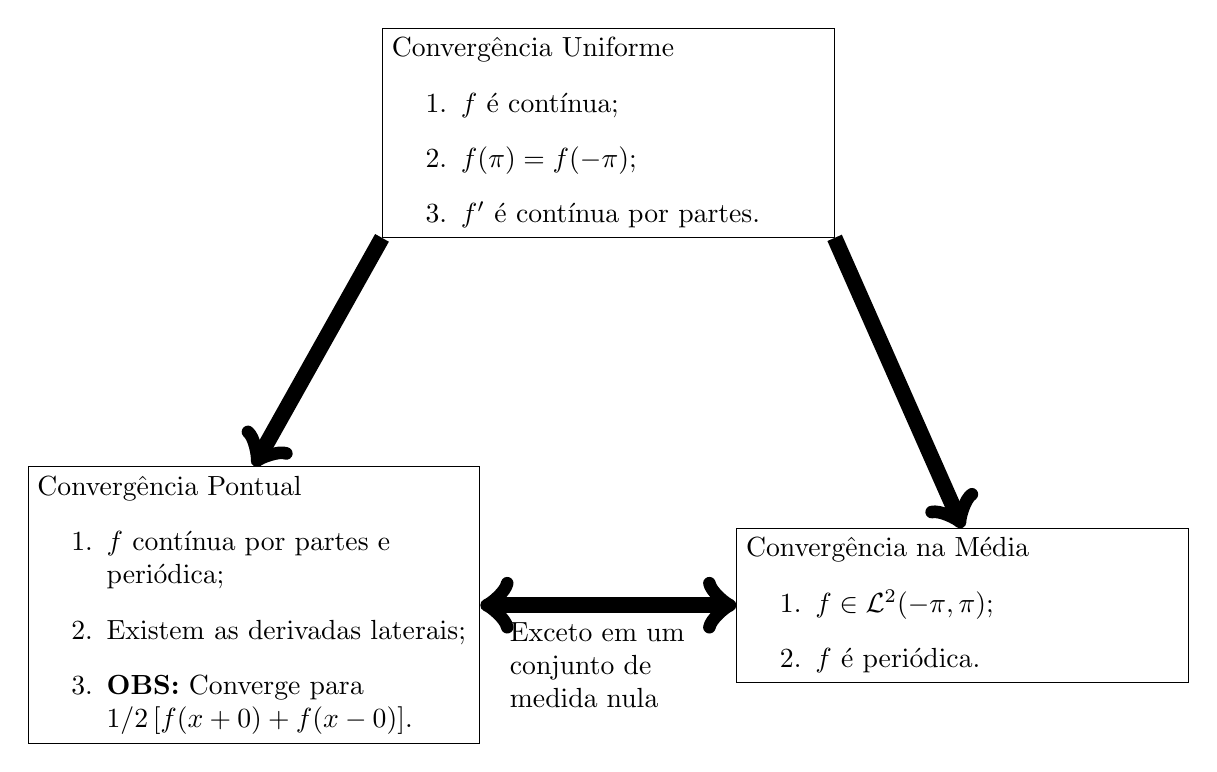
\begin{tikzpicture}
    \node[draw=black, text width=5.5cm] (U) at (0,0) {Convergência Uniforme
    \begin{enumerate}
      \item $f$ é contínua;
      \item $f(\pi) = f(-\pi)$;
      \item $f'$ é contínua por partes.
    \end{enumerate}};
    \node[draw=black, text width=5.5cm] (P) at (-4.5,-6) {Convergência Pontual
    \begin{enumerate}
      \item $f$ contínua por partes e periódica;
      \item Existem as derivadas laterais;
      \item \textbf{OBS:} Converge para $1/2 \left[ f(x + 0) + f(x - 0) \right]$.
    \end{enumerate}};
    \node[draw=black, text width=5.5cm] (M) at (4.5,-6) {Convergência na Média
    \begin{enumerate}
      \item $f \in \mathcal{L}^2(-\pi, \pi)$;
      \item $f$ é periódica.
    \end{enumerate}};
    \draw[->, line width=.2cm] (U.south west) -- (P.north);
    \draw[->, line width=.2cm] (U.south east) -- (M.north);
    \draw[<->, line width=.2cm] (P.east) -- (M.west) node[midway, below, text
    width=2.5cm] {Exceto em um conjunto de medida nula};
  \end{tikzpicture}
\end{center}

\section{Método de Fejér}
\begin{defi}
  Dadas as somas parciais $S_k(x) = \sum_{i = 0}^k \mu_i(x)$ para $k = 0, 1,
  \ldots, N - 1$, a soma de Cesàro (ou média C-1) é definida como a meia
  aritmética dessas somas parciais:
  \begin{dmath*}
    \sigma_N(x) = \frac{1}{N} \sum_{k = 0}^{N - 1} S_k(x).
  \end{dmath*}
  Dizemos que uma série é C-1 somável se existir o $\lim_{N \to \infty}
  \sigma_N(x)$.
\end{defi}
\begin{obs}
  Podemos definir a média C-2, etc, como a média aritmética das somas de
  Cesàro, ou seja,
  \begin{dmath*}
    \sigma_N^{(2)}(x) = \frac{1}{N} \sum_{k = 0}^{N - 1} \sigma_N(x),
  \end{dmath*}
  e dizer que a série é C-2 somável se existir $\lim_{N \to \infty}
  \sigma_N^{(2)}(x)$.
\end{obs}
\begin{exem}
  Considere $S_k(x) = \sum_{i = 0}^{k - 1} (-1)^i$, então
  \begin{dgroup*}
    \begin{dmath*}
      S_0 = 1,
    \end{dmath*}
    \begin{dmath*}
      S_1 = 1 - 1 = 0,
    \end{dmath*}
    \begin{dmath*}
      S_2 = 1 - 1 + 1 = 1, \vdots
    \end{dmath*}
  \end{dgroup*}
  e
  \begin{dgroup*}
    \begin{dmath*}
      S_0 = 1,
    \end{dmath*}
    \begin{dmath*}
      S_0 + S_1 = 1,
    \end{dmath*}
    \begin{dmath*}
      S_0 + S_1 + S_2 = 2, \ldots
    \end{dmath*}
  \end{dgroup*}
  Logo,
  \begin{dgroup*}
    \begin{dmath*}
      \sigma_0 = \frac{1}{1} 1 \hiderel{=} 1,
    \end{dmath*}
    \begin{dmath*}
      \sigma_1 = \frac{1}{2} 1 \hiderel{=} \frac{1}{2},
    \end{dmath*}
    \begin{dmath*}
      \sigma_2 = \frac{1}{3} 2 \hiderel{=} \frac{2}{3},
    \end{dmath*}
    \begin{dmath*}
      \sigma_3 = \frac{1}{4} 2 \hiderel{=} \frac{1}{2},
    \end{dmath*}
    \begin{dmath*}
      \sigma_4 = \frac{1}{5} 3 \hiderel{=} \frac{3}{5},
    \end{dmath*}
    \begin{dmath*}
      \sigma_5 = \frac{1}{6} 3 \hiderel{=} \frac{1}{2}, \ldots
    \end{dmath*}
    \begin{dmath*}
      \sigma_{2n} = \frac{n + 1}{2n + 1},
    \end{dmath*}
    \begin{dmath*}
      \sigma_{2n + 1} = \frac{1}{2}.
    \end{dmath*}
  \end{dgroup*}
  e como
  \begin{dgroup*}
    \begin{dmath*}
      \lim_{n \to \infty} \sigma_{2n + 1} = 1/2,
    \end{dmath*}
    \begin{dmath*}
      \lim_{n \to \infty} \sigma_{2n} = 1/2,
    \end{dmath*}
  \end{dgroup*}
  temos que a série $\sum_{i = 0}^\infty (-1)^i$ é C-1 somável e o resultado é
  $1/2$.
\end{exem}
\begin{obs}
  Usar a soma de Cesàro da série de Fourier.
  \begin{dgroup*}
    \begin{dmath*}
      \sigma_1 = \frac{a_0}{2},
    \end{dmath*}
    \begin{dmath*}
      \sigma_2 = \frac{1}{2} \left[ \frac{a_0}{2} + \left[ \frac{a_0}{2} +
      \left( a_1 \cos\left( x \right) + b_1 \sin\left( x \right) \right) \right]
      \right],
    \end{dmath*}
    \begin{dmath*}
      \sigma_3 = \frac{1}{3} \left[ \frac{a_0}{2} + \left[ \frac{a_0}{2} +
      \sum_{k = 1}^1 \left( a_k \cos\left( k x \right) + b_k \sin\left( k x
      \right) \right) \right] + \left[ \frac{a_0}{2} + \sum_{k = 1}^2 \left( a_k
      \cos\left( k x \right) + b_k \sin\left( k x \right) \right) \right]
      \right],
    \end{dmath*}
    \begin{dmath*}
      \sigma_N = \frac{1}{N} \left[ \frac{a_0}{2} + \left[ \frac{a_0}{2} +
      \sum_{k = 1}^1 \left( a_k \cos\left( k x \right) + b_k \sin\left( k x
      \right) \right) \right] \left[ \frac{a_0}{2} + \sum_{k = 1}^2 \left( a_k
      \cos\left( k x \right) + b_k \sin\left( k x \right) \right) \right]
      \vdots + \left[ \frac{a_0}{2} + \sum_{k = 1}^{N - 1} \left( a_k
      \cos\left( k x \right) + b_k \sin\left( k x \right) \right)
      \right]\right]
      = \left( \frac{N}{N} \right) \left( \frac{a_0}{2} \right) + \left(
      \frac{N - 1}{N} \right) \left( a_1 \cos\left( x \right) + b_1 \sin\left(
      x \right) \right) + \left( \frac{N - 2}{N} \left( a_2 \cos\left( 2 x
      \right) + b_2 \sin\left( 2 x \right) \right) \right) + \cdots + \left(
      \frac{N - \left( N - 1 \right)}{N} \right) \left( a_{N - 1} \cos\left(
      \left( N - 1 \right) x \right) + b_{N - 1} \sin\left( \left( N - 1
      \right) x \right) \right)
    \end{dmath*}
  \end{dgroup*}
  Portanto,
  \begin{dgroup*}
    \begin{dmath*}
      \sigma_N(x) = \frac{a_0}{2} + \sum_{k = 1}^{N - 1} \left( \alpha_k^N
      \cos\left( k x \right) + \beta_k^N \sin\left( k x \right) \right),
    \end{dmath*}
    \begin{dmath*}
      \alpha_k^N = \left( 1 - \frac{k}{N} \right) a_k,
    \end{dmath*}
    \begin{dmath*}
      \beta_k^N = \left( 1 - \frac{k}{N} \right) b_k.
    \end{dmath*}
  \end{dgroup*}

  Por outro lado, sabemos que
  \begin{dmath*}
    S_N(x) = \int_{-\pi}^\pi f(\xi) D_N(\xi - x) \vi{\xi},
  \end{dmath*}
  onde $D_N$ denota o núcleo de Dirichlet. Logo
  \begin{dmath*}
    \sigma_N(x) = \frac{1}{N} \sum_{k = 0}^{N - 1} \int_{-\pi}^\pi f(\xi)
    D_k(\xi - x) \vi{\xi}
  \end{dmath*}
  ou ainda
  \begin{dmath*}
    \sigma_N(x) = \int_{-\pi}^\pi f(\xi) F_N(\xi - x) \vi{\xi},
  \end{dmath*}
  onde
  \begin{dmath*}
    F_N(\mu) = \frac{1}{N} \sum_{k = 0}^{N - 1} D_k(\mu).
  \end{dmath*}

  Lembrando que $D_k(\mu) = \left[ \sin\left( k + 1/2 \right) \mu \right] /
  \left[ 2 \pi \sin\left( \mu/2 \right) \right]$, temos
  \begin{dmath*}
    \sin^2\left( \frac{\mu}{2} \right) F_N(\mu) = \frac{1}{N} \sin^2\left( \mu/2 \right)
    \sum_{k = 0}^{N - 1} \frac{\sin\left( k + 1/2 \right) \mu}{2 \pi \sin\left(
    \mu/2 \right)}
    = \frac{1}{2 \pi N} \sum_{k = 0}^{N - 1} \sin\left( \mu/2 \right) \sin\left(
    k + 1/2 \right) \mu
    = \frac{1}{2 \pi N} \sum_{k = 0}^{N - 1} \frac{1}{2} \left[ \cos\left( k +
    1/2 - 1/2 \right) \mu - \cos\left( k + 1/2 + 1/2 \right) \mu \right]
    = \frac{1}{4 \pi N} \sum_{k = 0}^{N - 1} \left( \cos\left( k \mu \right) -
    \cos\left( \left( k + 1 \right) \mu \right) \right)
    = \frac{1}{4 \pi N} \left( 1 - \cos\left( N \mu \right) \right)
    = \frac{1}{2 \pi N} \left( \frac{1 - \cos\left( N \mu \right)}{2} \right)
    = \frac{1}{2 \pi N} \sin^2\left( N \mu / 2 \right).
  \end{dmath*}
\end{obs}
\begin{defi}
  O núcleo de Fejér $F_N(\mu)$ é definido como
  \begin{dmath*}
    F_N(\mu) = \frac{1}{N} \sum_{k = 0}^{N - 1} D_k(\mu) = \frac{\sin^2\left( N
    \mu / 2 \right)}{2 \pi N \sin^2\left( \mu/2 \right)}.
  \end{dmath*}
\end{defi}

Antes de prosseguir, é importante notermos que:
\begin{lem}
  Temos que
  \begin{dgroup*}
    \begin{dmath*}
      \int_{-\pi}^\pi D_k(\mu) \vi{\mu} = 1,
    \end{dmath*}
    \begin{dmath*}
      \int_{-\pi}^\pi F_k\left( \mu \right) \vi{\mu} = 1.
    \end{dmath*}
  \end{dgroup*}
\end{lem}
\begin{proof}
  Sabendo que
  \begin{dmath*}
    D_k(\mu) = \frac{\sin\left( k + 1/2 \right) \mu}{2 \pi \sin\left( \mu/2
    \right)}
    = \left( 1 + 2 \sum_{j = 1}^{k - 1} \cos\left( j \mu \right) \right)
    \frac{1}{2 \pi}
  \end{dmath*}
  temos que
  \begin{dmath*}
    \int_{-\pi}^\pi D_k\left( \mu \right) \vi{\mu} = \frac{1}{2 \pi} \left[ \pi
    - \left( -\pi \right) + 2 \sum_{j = 1}^{k - 1} \left. \frac{\sin\left( j \mu
    \right)}{j} \right|_{-\pi}^\pi \right] = 1
  \end{dmath*}
  e
  \begin{dmath*}
    \int_{-\pi}^\pi F_k(\mu) \vi{\mu} = \frac{1}{k} \sum_{j = 0}^{k - 1}
    \int_{-\pi}^\pi D_j(\mu) \vi{\mu} = \frac{1}{k} k = 1. \qedhere
  \end{dmath*}
\end{proof}
\begin{teo}[Fejér] \label{teo:fejer}
  Seja $f(x)$ uma função contínua e periódica (de período $2\pi$) e seja
  $\sigma_N(x)$ a soma de Cesàro da série de Fourier de $f(x)$, ou seja,
  \begin{dmath*}
    \sigma_N(x) = \frac{a_0}{2} + \sum_{k = 1}^{N - 1} \left( \alpha_k^N
    \cos\left( k x \right) + \beta_k^N \sin\left( k x \right) \right),
  \end{dmath*}
  onde $\sigma_k^N = \left( 1 - k/N \right) a_k$ e $\beta_k^N = \left( 1 - k/N
  \right) b_k$. Então a sequência de funções $\sigma_n(x)$ converge para $f(x)$.
\end{teo}
\begin{proof}
  (mais fácil que Fourier pois $F_N(\mu) \geq 0$)
  \begin{dgroup*}
    \begin{dmath*}
      \sigma_N(x) = \int_{-\pi}^\pi f(\xi) F_N(\xi - x) \vi{\xi}
      = \int_{a - \pi}^{a + \pi} f(\xi) F_{N}(\xi - x) \vi{\xi}
      = \int_{x - \pi}^{x + \pi} f(\xi) F_N(\xi - x) \vi{\xi}
      = \int_{-\pi}^\pi f(x + \mu) F_N(\mu) \vi{\mu}
    \end{dmath*}
    \begin{dmath*}
      \sigma_N(x) - f(x) = \int_{-\pi}^\pi f(x + \mu) F_N(\mu) \vi{\mu} - f(x)
      \int_{-\pi}^\pi F_N(\mu) \vi{\mu}
      = \int_{-\pi}^\pi \left[ f(x + \mu) - f(x) \right] F_N(\mu) \vi{\mu}
      = \frac{1}{\pi N} \int_{-\pi}^\pi \left[ f(x + \mu) - f(x) \right]
      \frac{\sin^2\left( N \mu/2 \right)}{2 \sin^2\left( \mu/2 \right)} \vi{\mu}
    \end{dmath*}
  \end{dgroup*}
  Logo, como $f$ é contínua então $\forall \epsilon > 0, \exists \delta > 0$ tal
  que $| f(x + \mu) - f(x)| < \epsilon$ para $| x + \mu - x| = | \mu | <
  \delta$.
  \begin{dmath*}
    \left\| \sigma_N(x) - f(x) \right\| = \left| \int_{-\pi}^\pi \left( \ldots \right) \right|
    = \left| \int_{-\pi}^{-\delta} \left( \ldots \right) + \int_{-\sigma}^\sigma
    \left( \ldots \right) + \int_\sigma^\pi \left( \ldots \right) \right|
    \leq \underbrace{\left| \int_{-\pi}^{-\delta} \left( \ldots \right)
    \right|}_{|I_1|} + \underbrace{\left| \int_{-\sigma}^\sigma \left( \ldots
    \right) \right|}_{|I_2|} + \underbrace{\left| \int_\sigma^\pi \left( \ldots
    \right) \right|}_{|I_3|}
  \end{dmath*}
  Mas
  \begin{dgroup*}
    \begin{dmath*}
      \left\| I_2 \right\| \leq \int_{-\delta}^\delta \underbrace{| f(x + \mu) - f(x) |}_{< \epsilon} F_N(\mu) \vi{\mu}
      < \epsilon \int_{-\delta}^\delta \underbrace{F_N(\mu)}_{\geq 0} \vi{\mu}
      < \epsilon \underbrace{\int_{-\delta}^\delta F_N(\mu) \vi{\mu}}_{=1}
      < \epsilon,
    \end{dmath*}
    \begin{dmath*}
      \left\| I_1 \right\| \leq  \frac{1}{\pi N} \int_{-\pi}^{-\delta} | f(x + \mu) - f(x) |
      \frac{\sin^2\left( N \mu/2 \right)}{2 \sin^2\left( \mu/2 \right)} \vi{\mu}
      \leq \frac{2 M}{\pi N} \int_{-\pi}^{-\delta} \frac{\sin^2\left( N \mu/2
      \right)}{2 \sin^2\left( \mu/2 \right)} \vi{\mu}
      \intertext{onde $M = \max |f(x)|$}
      \leq \frac{2 M}{\pi N} \int_{-\pi}^{-\delta} \frac{1}{2 \sin^2\left( \mu/2
      \right)} \vi{\mu}
      \leq \frac{2 M}{\pi N} \int_{-\pi}^{-\delta} \frac{1}{2 \sin^2\left(
      \delta/2 \right)} \vi{\mu}
      = \frac{M}{\pi N \sin^2\left( \delta/2 \right)}
      \underbrace{\int_{-\pi}^{-\delta} \vi{\mu}}_{\pi - \delta < \pi}
      \leq \frac{M \pi}{\pi N \sin^2\left( \delta/2 \right)}
      \leq \frac{M}{N \sin^2\left( \delta/2 \right)},
      \intertext{e analogamente}
    \end{dmath*}
    \begin{dmath*}
      \left\| I_3 \right\| \leq \frac{M}{N \sin^2\left( \delta/2 \right)}.
    \end{dmath*}
  \end{dgroup*}
  Portanto,
  \begin{dgroup*}
    \begin{dmath*}
      |\sigma_N(x) - f(x)| \leq \epsilon + \frac{2 M}{N \sin^2\left( \delta/2 \right)},
    \end{dmath*}
    \begin{dmath*}
      \lim_{N \to \infty} | \sigma_N(x) - f(x) | \leq \epsilon
    \end{dmath*}
  \end{dgroup*}
  de onde concluímos que
  \begin{dmath*}
    \lim_{N \to \infty} \sigma_N(x) = f(x) \qedhere
  \end{dmath*}
\end{proof}

\section{Diferenciação e Integração}
\begin{teo}
  Seja $f(x)$ uma função contínua em $[-\pi,\pi]$ tal que $f(-\pi) = f(\pi)$ e
  seja $f'(x)$ contínua por partes e com derivadas laterais nesse intervalo.
  Então a série de Fourier de $f(x)$ é diferenciável e
  \begin{dmath*}
    f'(x) = \sum_{n = 1}^\infty n \left( -a_n \sin\left( n x \right) + b_n
    \cos\left( n x \right) \right)
  \end{dmath*}
\end{teo}
\begin{proof}
  Como $f'(x)$ satisfaz as condições do Teorema de Fourier
  (página~\pageref{teo:fourier}), ela possui a série de Fourier
  \begin{dmath*}
    f'(x) = \frac{\alpha_0}{2} + \sum_{n = 1}^\infty \left( \alpha_n \cos\left(
    n x \right) + \beta_n \sin\left( n x \right) \right).
  \end{dmath*}
  Mas
  \begin{dgroup*}
    \begin{dmath*}
      \alpha_0 = \frac{1}{\pi} \int_{-\pi}^\pi f'(x) \vi{x}
      = \frac{1}{\pi} \left[ f(\pi) - f(-\pi) \right]
      = 0,
    \end{dmath*}
    \begin{dmath*}
      \alpha_n = \frac{1}{\pi} \left[ \underbrace{\left. f(x) \cos\left( n x
      \right) \right|_{-\pi}^\pi}_{=0} + n \int_{-\pi}^\pi f(x) \sin\left( n x
      \right) \vi{x} \right]
      = n b_n
    \end{dmath*}
    \begin{dmath*}
      \beta_n = \frac{1}{\pi} \left[ \underbrace{\left. f(x) \sin\left( n x
      \right) \right|_{-\pi}^\pi}_{=0} - n \int_{-\pi}^\pi f(x) \cos\left( n x
      \right) \vi{x} \right]
      = -n a_n
    \end{dmath*}
  \end{dgroup*}
  de modo que
  \begin{dmath*}
    f'(x) = \sum_{n = 1}^\infty \left( n b_n \cos\left( n x \right) - n a_n
    \sin\left( n x \right) \right). \qedhere
  \end{dmath*}
\end{proof}
\begin{obs}
  Note que o teorema fornece apenas uma condição suficiente. Além disso, podemos
  ter série de Fourier para $f(x)$ e não para $f'(x)$ (nesse caso o termo $n$ no
  numerador diminui a taxa de convergência da série).
\end{obs}
\begin{exem}
  A função $f(x) = x$ possui a série de Fourier
  \begin{dmath*}
    x = 2 \sum_{n = 1}^\infty (-1)^{n + 1} \frac{\sin\left( n x \right)}{n}.
  \end{dmath*}
  Porém $f(-\pi) = -\pi \neq \pi f(\pi)$, de modo que as condições do teorema
  não são satisfeitas e nada podemos afirmar acerca da série de Fourier de
  $f'(x)$ usando esse teorema. Note que nesse caso que a derivada da série de
  Fourier não converge!
  \begin{dmath*}
    1 \neq 2 \sum_{n = 1}^\infty (-1)^{n + 1} \cos\left( n x \right).
  \end{dmath*}
\end{exem}
\begin{obs}
  Dentro das condições do teorema anterior, uma vez que $\lim_{n \to \infty}
  \alpha_n = 0$ e $\lim_{n \to \infty} \beta_n = 0$ (critério do termo geral),
  temos
  \begin{dgroup*}
    \begin{dmath*}
      \lim_{n \to \infty} n a_n = 0,
    \end{dmath*}
    \begin{dmath*}
      \lim_{n \to \infty} n b_n = 0.
    \end{dmath*}
  \end{dgroup*}
  Note que a série do exemplo anterior não satisfaz essas condições.
\end{obs}
\begin{teo}
  Seja $f(x)$ uma função contínua por partes em $(-\pi,\pi)$. Então,
  independentemente da série de Fourier de $f(x)$ convergir ou não, vale a
  seguinte igualdade:
  \begin{dmath*}
    \int_{-\pi}^x f(\xi) \vi{\xi} = \frac{1}{2} a_0 \left( x + \pi \right) +
    \sum_{n = 1}^\infty \frac{1}{n} \left[ a_n \sin\left( n x \right) - b_n
    \left( \cos\left( n x \right) - \cos\left( n \pi \right) \right) \right],
  \end{dmath*}
  quando $x \in [-\pi,\pi]$.
\end{teo}
\begin{proof}
  Seja
  \begin{dmath*}
    F(x) = \int_{-\pi}^x f(\xi) \vi{\xi} - \frac{a_0}{2} x.
  \end{dmath*}
  Se $f(x)$ é contínua por partes então $F(x)$ é contínua. Além disso $F'(x) =
  f(x) - a_0/2$, de modo que $F'(x)$ é contínua por partes. Podemos ainda notar
  que $F(-\pi) = -a_0 / 2 (-\pi) = \pi a_0 / 2$ e
  \begin{dmath*}
    F(\pi) = \int_{-\pi}^\pi f(\xi) \vi{\xi} - \frac{a_0}{2} \pi
    = a_0 \pi - \frac{a_0}{2} \pi
    = \frac{a_0 \pi}{2}
  \end{dmath*}
  ou seja, $F(\pi) = F(-\pi)$. Temos com isso que $F(x)$ satisfaz as condições
  do teorema de Fourier e possui portanto a série de Fourier
  \begin{dgroup*}
    \begin{dmath*}
      F(x) = \frac{A_0}{2} + \sum_{n = 1}^\infty \left( A_n \cos\left( n x
      \right) + B_n \sin\left( n x \right) \right),
    \end{dmath*}
    \begin{dmath*}
      A_n = \frac{1}{\pi} \int_{-\pi}^\pi F(x) \cos\left( n x \right) \vi{x},
    \end{dmath*}
    \begin{dmath*}
      B_n = \frac{1}{\pi} \int_{-\pi}^\pi F(x) \sin\left( n x \right) \vi{x}.
    \end{dmath*}
  \end{dgroup*}
  Para $n \neq 0$,
  \begin{dgroup*}
    \begin{dmath*}
      A_n = \frac{1}{n} \int_{-\pi}^\pi \left[ \int_{-\pi}^x f(\xi) \id(\xi) -
      \frac{a_0}{2} x \right] \cos\left( n x \right) \vi{x}
      = \frac{1}{\pi} \underbrace{\left. F(x) \frac{\sin\left( n x \right)}{n}
      \right|_{-\pi}^\pi}_{=0} - \frac{1}{\pi} \int_{-\pi}^\pi \frac{\sin\left(
      n x \right)}{n} \left[ f(x) - \frac{a_0}{2} \right] \vi{x}
      = - \frac{1}{n \pi} \int_{-\pi}^\pi f(x) \sin\left( n x \right) \vi{x} +
      \frac{a_0}{2 n \pi} \underbrace{\int_{-\pi}^\pi \sin\left( n x \right)
      \vi{x}}_{=0}
      = -\frac{1}{n} b_n,
    \end{dmath*}
    \begin{dmath*}
      B_n = \frac{1}{n} \int_{-\pi}^\pi \left[ \int_{-\pi}^x f(\xi) \vi{\xi} -
      \frac{a_0 x}{2} \right] \sin\left( n x \right) \vi{x}
      = \underbrace{-\frac{1}{\pi} \left. F(x) \frac{\cos\left( n x \right)}{n}
      \right|_{-\pi}^\pi}_{=0} + \frac{1}{n \pi} \int_{-\pi}^\pi \cos\left( n x
      \right) \left[ f(x) - \frac{a_0}{2} \right] \vi{x}
      = \frac{1}{n \pi} \int_{-\pi}^\pi \cos\left( n x \right) f(x) \vi{x} -
      \frac{a_0}{2 n \pi} \underbrace{\int_{-\pi}^\pi \cos\left( n x \right)
      \vi{x}}_{=0}
      = \frac{1}{n} a_n
    \end{dmath*}
  \end{dgroup*}
  e portanto
  \begin{dmath*}
    F(x) = \frac{A_0}{2} + \sum_{n = 1}^\infty \left( \frac{-b_n}{n} \cos\left(
    n x \right) + \frac{a_n}{n} \sin\left( n x \right) \right).
  \end{dmath*}
  Tomando $x = \pi$,
  \begin{dmath*}
    F(\pi) = \frac{a_0 \pi}{2} = \frac{A_0}{2} \sum_{n = 1}^\infty \left(
    \frac{-b_n}{n} \cos\left( n \pi \right) + \frac{a_n}{n}
    \underbrace{\sin\left( n \pi \right)}_{=0} \right)
  \end{dmath*}
  e portanto
  \begin{dmath*}
    \frac{A_0}{2} = \frac{a_0 \pi}{2} + \sum_{n = 1}^\infty \frac{b_n}{n}
    \cos\left( n \pi \right)
  \end{dmath*}
  de modo que
  \begin{dmath*}
    \int_{-\pi}^x f(\xi) \vi{\xi} - \frac{a_0 x}{2} = \frac{a_0 \pi}{2} +
    \sum_{n = 1}^\infty \frac{1}{n} \left[ a_n \sin\left( n x \right) - b_n
    \left( \cos\left( n x \right) - \cos\left( n \pi \right) \right) \right].
    \qedhere
  \end{dmath*}
\end{proof}
\begin{obs}
  Note que no caso da integração o termo $n$ no denominador aumenta a taxa de
  convergência.
\end{obs}
\begin{exem}
  A série de $f(x) = x$ é
  \begin{dmath*}
    x = 2 \sum_{n = 1}^\infty (-1)^{n + 1} \frac{\sin\left( n x \right)}{n}.
  \end{dmath*}
  Tomando $\int_0^x f(\xi) \vi{\xi}$ temos
  \begin{dmath*}
    x^2 = 4 \sum_{n = 1}^\infty \frac{(-1)^n}{n^2} \cos\left( n x \right) - 4
    \sum_{n = 1}^\infty \frac{(-1)^n}{n^2}
  \end{dmath*}
  que é justamente a série obtida na página~\pageref{exem:fourier:x^2} uma vez
  que $\sum_{n = 1}^\infty (-1)^n / (n^2) = -\pi^2 / 12$.
\end{exem}

\section{Fenômeno de Gibbs}
Para ilustrar o fenômeno de Gibbs, vamos considerar uma onda quadrada periódica
representada por
\begin{dmath*}
  f(x) = \begin{cases}
    h/2, & 0 < x < \pi, \\
    -h/2, & -\pi < x < 0.
  \end{cases}
\end{dmath*}
e ilustrada na Figura
\begin{figure}[!htb]
  \centering
  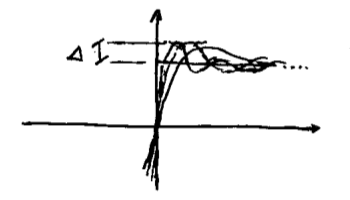
\includegraphics[width=.5\textwidth]{figuras/05-0}
  \begin{flushright}
    Imagem em domínio público de Johannes Rössel e disponível em
    \url{http://en.wikipedia.org/wiki/File:Gibbs_phenomenon_10.svg}.
  \end{flushright}
  \caption{Ilustração do Fenômeno de Gibbs para onda quadrada.}
  \label{fig:fenom_gibbs}
\end{figure}
% TODO Terminar de digitar a seção sobre o Fenômeno de Gibbs do arquivo M2S12-5.

\section{Teorema da Aproximação de Weierstrass}
\begin{teo}
  Seja $f(x)$ contínua em $a \leq x \leq b$. Então para todo $\epsilon > 0$
  existe um polinômio $P(x)$ tal que $|P(x) - f(x)| \leq \epsilon, \forall x \in
  [a,b]$.
\end{teo}
\begin{proof}
  Dado $f(x)$, $x \in [a,b]$, podemos definir $g(t)$ para $t \in [-\pi/2,
  \pi/2]$ através de
  \begin{dmath*}
    g(t) = f\left[ \left( \frac{b - a}{\pi} t + \left( \frac{b - a}{2} \right)
    \right) \right].
  \end{dmath*}
  Podemos ainda definir uma extensão de $g(t)$ para $x \in [-\pi, \pi]$, que
  denotaremos por $G(t)$, e de modo que $G(-\pi) = G(\pi)$. Podemos além disso
  considerar para os demais pontos a extensão periódica de $G(t)$. Nessas
  condições o Teorema de Fejér (página~\pageref{teo:fejer}) nos garante que a
  sequência $\sigma_N(t)$,
  \begin{dmath*}
    \sigma_N(t) = \frac{a_0}{2} + \sum_{k = 1}^{N - 1} \left( \alpha_k^N
    \cos\left( k t \right) + \beta_k^N \sin\left( k t \right) \right),
  \end{dmath*}
  converge para $G(t)$, ou seja, $\forall \epsilon > 0$, existe $N_0 > 0$ tal
  que
  \begin{dmath*}
    | \sigma_N(t) - G(t) | < \epsilon/2
  \end{dmath*}
  para $N > N_0$. Por outro lado, pelo Teorema de Taylor, existem polinômios
  $R_n^k(t)$ e $S_n^k(t)$ de grau $n$ tais que
  \begin{dgroup*}
    \begin{dmath*}
      | \cos\left( k t \right) - R_n^k(t) | < \epsilon',
    \end{dmath*}
    \begin{dmath*}
      | \sin\left( k t \right) - S_n^k(t) | < \epsilon'',
    \end{dmath*}
  \end{dgroup*}
  para $n > N_1$. Portanto, existe um polinômio $Q_N(t)$, que é uma combinação
  dos polinômios $R_n^k(t)$ e $S_n^k(t)$, tal que
  \begin{dmath*}
    | \sigma_N(t) - Q_N(t) | < \epsilon/2.
  \end{dmath*}
  Com isso,
  \begin{dmath*}
    | G(t) - Q_N(t) | = | G(t) - \sigma_N(t) + \sigma_N(t) - Q_N(t) |
    \leq \underbrace{| G(t) - \sigma_N(t) |}_{< \epsilon/2} + \underbrace{|
    \sigma_N(t) - Q_N(t) |}_{< \epsilon/2}
  \end{dmath*}
  e portanto $| G(t) - Q_N(t) | < \epsilon$ para $t \in [-\pi, \pi]$ e $| g(t) -
  Q_N(t) | < \epsilon$ para $t \in [-\pi/2, \pi/2]$ ou, definindo $P_N(x) =
  Q_N\left[ \left( \pi / \left( b - a \right) \right) x - \left( \pi / 2 \right)
  \left( \left( b + a \right) / \left( b - a \right) \right) \right]$,
  \begin{dmath*}
    | f(x) - P_N(x) | < \epsilon
  \end{dmath*}
  para $x \in [a, b]$.
\end{proof}

% Filename: cap02@notas_de_aula.tex
% This code is part of 'Notas de aula n\~{a}o oficiais de MS650 e F620'
% 
% Description: This file correspond to part of the textbook using in the course.
% 
% Created: 01.09.12 10:43:56 AM
% Last Change: 01.09.12 10:43:56 AM
% 
% Authors:
% - Raniere Silva, r.gaia.cs@gmail.com
% 
% Copyright (c) 2012, Raniere Silva. All rights reserved.
% 
% This work is licensed under the Creative Commons Attribution-NonCommercial-NoDerivs 3.0 Unported License. To view a copy of this license, visit http://creativecommons.org/licenses/by-nc-nd/3.0/.
%
% This work is distributed in the hope that it will be useful, but WITHOUT ANY WARRANTY; without even the implied warranty of MERCHANTABILITY or FITNESS FOR A PARTICULAR PURPOSE.
%
\chapter{Série de Fourier Generalizadas}
\section{O Problema de Sturm-Liouville (PSL)}
Vamos recordar alguns fatos básicos sobre o PSL. Seja
\begin{align*}
    L[y] &= \frac{\id{}}{\id{x}}\left[ p(x) \frac{\id{y}}{\id{x}} \right] - q(x) y.
\end{align*}
O PSL consiste na equação diferencial
\begin{align*}
    L[y] + \lambda p(x) y &= 0, & a \leq x \leq b
\end{align*}
com condições apropriadas conforme o problema seja regular ou singular. Uma solução $y$ não-trivial é dita uma auto-função e a constante $\lambda$ correspondente um auto-valor.

O PSL regular corresponde ao caso em que $p(x) > 0$, $\rho(x) > 0$, $p, p', q, \rho$ são contínuas em $x \in [a,b]$. Nesse caso as condições adequadas são:
\begin{enumerate}
    \item para condições de contorno homogêneas:
        \begin{align*}
            \begin{cases}
                \alpha_1 y(a) + \beta_1 y'(a) = 0, \\
                \alpha_2 y(b) + \beta_2 y'(b) = 0.
            \end{cases}
        \end{align*}
    \item para condições periódicas:
        \begin{align*}
            \begin{cases}
                y(a) = y'(b), \\
                y'(a) = y'(b).
            \end{cases}
        \end{align*}
    \item $y$ e $y'$ são limitadas (para $x \to a$ ou $x \to \pm \infty$ conforme o caso).
\end{enumerate}

E o PSL singular corresponde as
\begin{enumerate}
    \item $p(a) = 0$ ou $p(a) = 0$ e/ou $p(b) = 0$ ou $p(b) = 0$.
    \item $-\infty < x < \infty$, $0 \leq x \leq \infty$ e $-\infty < x \leq 0$.
\end{enumerate}

\begin{teo}
    As autofunções correspondentes a diferentes autovalores de um PSL regular com condição de contorno homoêneas ou periódicas são ortogonais com peso $\rho(x)$ em $[a,b]$, ou seja,
    \begin{align*}
        \int_a^b \rho(x) u(x) v(x) \id{x} = 0.
    \end{align*}
    O mesmo vale para as autofunções de quadrado integrável de um PSL singular com a condição que estas autofunções e suas derivadas primeiras sejam limitadas nos extremos.
\end{teo}
\begin{proof}
    % TODO Escrever prova.
    Ver curso de MS410.
\end{proof}
\begin{exem}
    Considere o PSL dado por
    \begin{align*}
        \begin{cases}
            y'' + \lambda y = 0, & -\pi < x < \pi, \\
            y(-\pi) = y(\pi), \\
            y(-\pi) = y'(\pi).
        \end{cases}
    \end{align*}

    Esse PSL tem autovalores $\lambda = n^2$, para $n = 0, 1, 2, \ldots$ e auto-funções $\left\{ 1, \cos\left( n x \right), \sin\left( n x \right) \right\}$. Note que temos duas autofunções para o mesmo autovalor para $n = 1, 2, \ldots$. Logo, os autovalores não são simples no caso periódico.

    Denotando
    \begin{align*}
        \phi_1(x) &= 1, & \phi_{2n}(x) &= \sin\left( n x \right), & \phi_{2n + 1}(x) &= \cos\left( n x \right)
    \end{align*}
    para $n = 1, 2, \ldots$ temos que o auto-valor correspondente a $\phi_k(x)$ é
    \begin{align*}
        \lambda_k &= \left( \left[ \frac{k}{2} \right] - 1 \right)^2
    \end{align*}
    onde $\left[ a \right]$ denota a parte inteira de $a$.

    A relação de ortogonalidade é
    \begin{align*}
        \int_{-\pi}^\pi \phi_n(x) \phi_m(x) \id{x} &= 0,
    \end{align*}
    para $n \neq m$, ou seja, as autofunções são ortogonais com peso $\rho(x) = 1$.
\end{exem}
\begin{exem}
    Considere o PSL dado por
    \begin{align*}
        \begin{cases}
            \left[ \left( 1 - x^2 \right) y' \right]' + \lambda y = 0, & -1 < x < 1 \\
            \lim_{x \to \pm 1} | y(x) | < \infty, \\
            \lim_{x \to \pm 1} | y'(x) | < \infty.
        \end{cases}
    \end{align*}

    Esse é um PSL singular cujos autovalores são $\lambda = n \left( n + 1 \right)$ para $n = 0, 1, 2, \ldots$ e as correspondentes autofunções são os polinômios de Legendre $P_n(x)$ definidos por
    \begin{align*}
        P_n(x) &= \frac{1}{2^n n!} \frac{\id{}^n}{\id{x^n}}\left( x^2 - 1 \right)^n
    \end{align*}
    para $n = 1, 2, \ldots$ e $P_0(x) = 1$. Logo,
    \begin{align*}
        P_1(x) &= x, \\
        P_2(x) &= \left( 1/2 \right) \left( 3 x^2 - 1 \right), \\
        P_3(x) &= \left( 1/2 \right) \left( 5 x^3 - 3 x \right), \ldots
    \end{align*}
\end{exem}

\section{Expansão ortogonais}
Sejam $\left\{ \phi_n(x) \right\}$ para $n = 1, 2, \ldots$ funções de quadrado integrável com peso $\rho(x)$ em $[a,b]$,
\begin{align*}
    \int_a^b \rho(x) \left[ \phi_n(x) \right]^2 \id{x} < \infty
\end{align*}
e ortogonais (com peso $\rho(x)$) para $n \neq m$,
\begin{align*}
    \int_a^b \rho(x) \phi_n(x) \phi_m(x) \id{x} = 0
\end{align*}
para $n \neq m$.

Vamos denotar por $\langle \cdot, \cdot \rangle$ o produto escalar em $L_p^2(a, b)$:
\begin{align*}
    \langle f,g \rangle &= \int_a^b \rho(x) f(x) g(x) \id{x}.
\end{align*}

Agora vamos supor que uma função $f(x)$ pode ser escrita como o limite de uma série uniformimente convergente de múltiplos de $\phi_n(x)$, ou seja,
\begin{align*}
    f(x) &= \sum_{k = 1}^\infty c_n \phi_n(x).
\end{align*}
Com isso temos que
\begin{align*}
    \langle f,\phi_m \rangle &= \int_a^b \rho(x) f(x) \phi_m(x) \id{x} \\
    &= \int_a^b \left( \sum_{n = 1}^\infty c_n \phi_n(x) \right) \phi_m(x) \rho(x) \id{x} \\
    &= \sum_{n = 1}^\infty c_n \int_a^b \phi_n(x) \phi_m(x) \rho(x) \id{x} \\
    &= \sum_{n = 1}^\infty c_n \delta_{nm} \int_a^b \left[ \phi_m(x) \right]^2 \rho(x) \id{x} \\
    &= c_n \int_a^b \left[ \phi_m(x) \right]^2 \rho(x) \id{x} \\
    &= c_m \langle \phi_m, \phi_m \rangle \\
    &= c_m \| \phi_m \|^2,
\end{align*}
ou seja,
\begin{align*}
    c_n &= \frac{\langle f, \phi_n \rangle}{\| \phi_n \|^2}.
\end{align*}

\begin{exem}
    Para a série de Fourier temos
    \begin{align*}
        \| \phi_1(x) \|^2 &= 2 \pi, & \| \phi_k \|^2 &= \pi
    \end{align*}
    para $k = 2, 3, \ldots$, e portanto
    \begin{align*}
        c_1 &= \frac{\langle f, \phi_1 \rangle}{2\pi} \\
        &= \frac{1}{2\pi} \int_{-\pi}^\pi f(x) \id{x} \\
        &= \frac{a_0}{2}, \\
        c_{2n} &= \frac{\langle f, \phi_{2n} \rangle}{\pi} \\
        &= \frac{1}{\pi} \int_{-\pi}^\pi f(x) \sin\left( n x \right) \id{x} \\
        &= b_n, \\
        c_{2n + 1} &= \frac{\langle f, \phi_{2n + 1} \rangle}{\pi} \\
        &= \frac{1}{\pi} \int_{-\pi}^\pi f(x) \cos\left( n x \right) \id{x} \\
        &= a_n.
    \end{align*}
\end{exem}

Diremos que $c_n$ é o coeficiente de Fourier generalizado da série de Fourier generalizada $f(x) = \sum_{n = 1}^\infty c_n \phi_n(x)$.

Dada uma soma
\begin{align*}
    s_N(x) &= \sum_{n = 1}^N \gamma_n \phi_n(x),
\end{align*}
o desvio total quadrático $\Delta_N$
\begin{align*}
    \Delta_N &= \| s_N - f \|^2 \\
    &= \int_a^b \rho(x) \left[ s_N(x) - f(x) \right]^2 \id{x}
\end{align*}
é minimizado quando $\gamma_n = c_n$, ou seja, $s_N = S_N$, que é a $N$-ésima soma parcial da série de Fourier generalizada. De fato:
\begin{align*}
    \Delta_N &= \langle s_N - f, s_N - f \rangle \\
    &= \langle s_N, s_N \rangle - 2 \langle s_N, f \rangle - \langle f, f \rangle, \\
    \langle s_N, s_N \rangle &= \sum_{n = 1}^`N \sum_{m = 1}^N \gamma_n \gamma_m \langle \phi_n, \phi_m \rangle \\
    &= \sum_{n = 1}^N \gamma_n^2 \| \phi_n \|^2, \\
    \langle s_N, f \rangle &= \sum_{n = 1}^N \gamma_n \langle \phi_n, f \rangle.
\end{align*}
Portanto,
\begin{align*}
    \frac{\partial \Delta_N}{\partial \gamma_k} &= 2 \gamma_k \| \phi_k \|^2 - 2 \langle \phi_k, f \rangle = 0
\end{align*}
que implica em
\begin{align*}
    \gamma_k = \frac{\langle \phi_k, f \rangle}{\| \phi_k \|^2} &= c_k.
\end{align*}

Como $\Delta_N \geq 0$, para $\Delta_N^{\min{}}$ temos
\begin{align*}
    0 \leq \Delta_N^{\min{}} \\
    &= \sum_{n = 1}^N c_n^2 \| \phi_n \|^2 - 2 \sum_{n = 1}^N c_n \langle \phi_n, f \rangle + \| f \|^2 \\
    &= \sum_{n = 1}^N \frac{\langle \phi_n, f \rangle^2}{\| \phi_n \|^2} \| \phi_n \|^2 - 2 \sum_{n = 1}^\infty \frac{\langle \phi_n, f \rangle}{\| \phi_n \|^2} + \| f \|^2,
\end{align*}
ou seja,
\begin{align*}
    \sum_{n = 1}^N \frac{\langle \phi_n, f \rangle^2}{\| \phi_n \|^2} \leq \| f \|^2
\end{align*}
e com os argumentos conhecidos para a série de Fourier segue a desigualdade de Bessel generalizada
\begin{align*}
    \sum_{n = 1}^\infty \frac{\langle \phi_n, f \rangle^2}{\| \phi_n \|^2} \leq \| f \|^2.
\end{align*}

Dizemos que $S_N(x)$ converge na média para $f(x)$ se
\begin{align*}
    \lim_{N \to \infty} \| S_N - f \|^2 &= \lim_{N \to \infty} \left\| \sum_{n = 1}^N c_n \phi_n - f \right\|^2 = 0
\end{align*}
e nesse caso dizemos que $\left\{ \phi_n(x) \right\}$ é completo. Uma condição necessária e suficiente para isso é valer a identidade de Parseval generalizada,
\begin{align*}
    \sum_{n = 1}^\infty \frac{\langle \phi_n, f \rangle^2}{\| \phi_n \|^2} &= \| f \|^2,
\end{align*}
ou ainda
\begin{align*}
    \sum_{n = 1}^\infty c_n^2 \| \phi_n \|^2 &= \| f \|^2.
\end{align*}

\section{Polinômios ortogonais}
seja $\left\{ P_n(x) \right\}$, $n = 0, 1, 2, \ldots$, uma sequ\^{e}ncia de polin\^{o}mios tais que $P_n(x)$ seja de graun $n$ e que sejam ortogonais em $[a,b]$ para $n \neq m$,
\begin{align*}
    \langle P_n, P_m \rangle &= \int_a^b \rho(x) P_n(x) P_m(x) \id{x} = 0.
\end{align*}
\begin{exem}
    V\'{a}rios polin\^{o}mios ortogonais surgem como autofun\c{c}\~{o}es de PSL; alguns exemplos s\~{a}o:
    \begin{align*}
        \frac{\id{}}{\id{x}}\left[ p(x) \frac{\id{y}}{\id{x}} \right] - q(x) y + \lambda \rho(x) y &= 0.
    \end{align*}
\end{exem}
\begin{table}[!htb]
    \centering
    \caption{Polin\^{o}mios otogonais que surgem como autofun\c{c}\~{o}es de PSL.}
    \label{tab:pol_ort_PSL}
    \begin{tabular}{|c|c|c|c|c|c|}
        \hline
        polin\^{o}mio $P_n(x)$ & $p(x)$ & $q(x)$ & $\rho(x)$ & $\lambda$ & $[a,b]$ \\ \hline
        Legendre $P_n(x)$ & $\left( 1 - x^2 \right)$ & $0$ & $1$ & $n \left( n + 1 \right)$ & $-1 \leq x \leq 1$ \\ \hline
        Chebyshev $T_n(x)$ & $\left( 1 - x^2 \right)^{1/2}$ & $0$ & $\left( 1 - x^2 \right)^{-1/2}$ & $n^2$ & $-1 \leq x \leq 1$ \\ \hline
        Hermite $H_n(x)$ & $\exp(-x^2)$ & $0$ & $\exp(-x^2)$ & $2n$ & $-\infty < x < \infty$ \\ \hline
        Laguerre $L_n(x)$ & $x \exp(-x)$ & $0$ & $\exp(-x)$ & $n$ & $0 \leq x < \infty$ \\ \hline
    \end{tabular}
\end{table}
\begin{teo}
    Uma sequ\^{e}ncia de polin\^{o}mios ortogonais em um intervalo finito $a \leq x \leq b$ \'{e} completa.
\end{teo}
\begin{proof}
    Seja $\left\{ P_n(x) \right\}$ uma sequ\^{e}ncia de polin\^{o}mios ortogonais tais que $P_n(x)$ \'{e} de grau $n$ e seja $p_n(x)$ um polin\^{o}mio de grau $n$ arbitr\'{a}rio. Ent\~{a}o existe $c_n$ tal que $p_n(x) - c_n P_n(x)$ seja um polin\^{o}mio de grau $n - 1$. Da mesma forma, existe $c_{n - 1}$ tal que $\left( p_n(x) - c_n P_n(x) \right) - c_{n - 1} P_{n - 1}(x)$ seja um polin\^{o}mio de grau $n - 2$. Dessa forma podemos escrever
    \begin{align*}
        p_n(x) &= \sum_{k = 0}^n c_k P_k(x).
    \end{align*}
    Mas, pelo teorema da aproxima\c{c}\~{a}o de Weierstrass
    \begin{align*}
        | f(x) - p_n(x) | < \epsilon
    \end{align*}
    para $a \leq x \leq b$. Logo,
    \begin{align*}
        \int_a^b \left[ f(x) - p_n(x) \right]^2 \rho(x) \id{x} < \epsilon^2 \int_a^b \underbrace{\rho(x)}_{>0} \id{x} < \epsilon',
    \end{align*}
    ou seja,
    \begin{align*}
        \lim_{n \to \infty} \| f - \sum_{k = 0}^n c_k P_k \| &= 0,
    \end{align*}
    de modo que $\left\{ P_n(x) \right\}$, $n = 0, 1, 2, \ldots$ \'{e} completo.
\end{proof}

\section{S\'{e}rie de Fourier-Legendre}
Uma s\'{e}rie de Fourier-Legendre \'{e} uma s\'{e}rie da forma $f(x) = \sum_{n = 0}^\infty c_n P_n(x)$, onde $P_n(x)$ s\~{a}o polin\^{o}mios de Legendre, dados por $P_0(x) = 1$ e
\begin{align*}
    P_n(x) &= \frac{1}{2^n n!} \frac{\id{}^n}{\id{x}^n}\left( x^2 - 1 \right)^n,
\end{align*}
$n = 1, 2, \ldots$, que \'{e} chamada f\'{o}rmula de Rodrigues.
\begin{prop}
    As seguintes rela\c{c}\~{o}es e identidades s\~{a}o v\'{a}lidas:
    \begin{enumerate}
        \item $P_(x) = (-1)^n P_n(-x)$ e $P_n(1) = 1$;
        \item $P_n'(x) = x P_{n - 1}'(x) + n P_{n - 1}(x)$ para $n \geq 1$;
        \item $n P_n(x) = n x P_{n - 1}(x) + \left( x^2 - 1 \right) P_{n - 1}'(x)$ para $n \geq 1$;
        \item $P_{n + 1}'(x) - P_{n - 1}'(x) = \left( 2 n + 1 \right) P_n(x)$ para $n \geq 1$;
        \item $\left[ \id{}\left[ (1 0 x^2) P_n'(x) \right] \right] / \id{x} + n (n + 1) P_n(x) = 0$;
        \item $(n + 1) P_{n + 1}(x) = (2n + 1) x P_n(x) - n P_{n - 1}(x)$ para $n \geq 1$;
        \item $(1 - x^2) (P_n')^2 + n^2 P_n^2 = (1 - x^2) (P_{n - 1}')^2 + n^2 P_{n - 1}^2$ para $n \geq 1$;
        \item $\left[ (1 - x^2) / n^2 \right] (P_n')^2 + P_n^2 \leq 1$ para $n \geq 1$ e $|x| \leq 1$;
        \item $| P_n(x) | \leq 1$ para $|x| \leq 1$;
        \item $\int_{-1}^1 P_n(x) P_m(x) \id{x} = \left[ 2 / \left( 2 n + 1 \right) \right] \delta_{nm}$.
    \end{enumerate}
\end{prop}
\begin{proof}
    % TODO Escrever a demonstra\c{c}\~{a}o das identidades.
\end{proof}
\begin{exem}
    Fourier-Legendre para $f(x) = x^2$.
    \begin{align*}
        x^2 &= \sum_{n = 0}^\infty c_n P_n(x) \\
        \langle x^2, P_m \rangle &= \sum_{n = 0}^\infty c_n \langle P_n, P_m \rangle \\
        &= c_m \frac{2}{2m + 1} \\
        c_m &= \frac{2m + 1}{2} \langle x^2, P_m \rangle \\
        &= \frac{2m + 1}{2} \int_{-1}^1 x^2 P_m(x) \id{x} \\
        \langle x^2, P_m \rangle &= \langle x^2, \frac{P_{m + 1}}{m + 1} - \frac{x P_m'}{m + 1} \rangle \\
        &= \frac{1}{m + 1} \langle x^2, P_{m + 1}' \rangle - \frac{1}{m + 1} \langle x^3, P_m' \rangle \\
        &= \frac{1}{m + 1} \left[ \left. x^2 P_{m + 1} \right|_{-1}^1 - 2 \langle x, P_{m + 1} \rangle \right] - \frac{1}{m + 1} \left[ \left. x^3 P_m \right|_{-1}^1 - 3 \langle x^2, P_m \rangle \right] \\
        \begin{split}
            &= \frac{1}{m + 1} \left[ \underbrace{P_{m + 1}(1)}_{1} \underbrace{P_{m + 1}(-1)}_{(-1)^{m + 1}} - 2 \langle x, P_{m + 1} \rangle \right] \\
            &\quad {}- \frac{1}{m + 1} \left[ \underbrace{P_{m + 1}(1)}_{1} + \underbrace{P_m(-1)}_{(-1)^m} - 3 \langle x^2, P_m \rangle \right]
        \end{split} \\
        &= \frac{1}{m + 1} \left[ 1 - (-1)^{m + 1} - 1 - (-1)^m \right] - \frac{2}{m + 1} \langle x, P_{m + 1} \rangle + \frac{3}{m + 1} \langle x^2, P_m \rangle.
    \end{align*}
    Portanto,
    \begin{align*}
        \left( \frac{3}{m + 1} - 1 \right) \langle x^2, P_m \rangle &= \frac{2}{m + 1} \langle x, P_{m + 1} \rangle \\
        \left( 2 - m \right) \langle x^2, P_m \rangle &= 2 \langle x, P_{m + 1} \rangle.
    \end{align*}
    Mas,
    \begin{align*}
        P_1(x) = x \Rightarrow \left( 2 - m \right) \langle x^2, P_m \rangle = 2 \langle P_1, P_{m + 1} \rangle
    \end{align*}
    e portanto
    \begin{align*}
        m = 0 &\Rightarrow 2 \langle x^2, P_0 \rangle = 2 \langle P_1, P_1 \rangle = 4 / 3 \\
        m \neq 0 &\Rightarrow \left( 2 - m \right) \langle x^2, P_m \rangle = 0.
    \end{align*}
    % TODO Terminar de escrever exemplo. Falta p\'{a}gina 83.
\end{exem}

\section{S\'{e}rie de Fourier-Bessel}
A equa\c{c}\~{a}o de Bessel de ordem $\nu$ ($\nu > 0$) \'{e}
\begin{align*}
    x^2 y'' + x y' + \left( x^2 - \nu^2 \right) y &= 0.
\end{align*}
Sua solu\c{c}\~{a}o geral \'{e} da forma
\begin{align*}
    y &= c_1 J_\nu(x) + c_2 Y_\nu(x),
\end{align*}
onde $J_\nu(x)$ \'{e} a fun\c{c}\~{a}o de Bessel de primeira esp\'{e}cie de ordem $\nu$ e $Y_\nu(x)$ \'{e} a fun\c{c}\~{a}o de Bessel de segunda esp\'{e}cie de ordem $\nu$ ou fun\c{c}\~{a}o de Neumann de ordem $\nu$. Para $J_\nu(x)$ temos
\begin{align*}
    J_\nu(x) &= \sum_{k = 0}^\infty \frac{(-1)^k}{\Gamma(k + \nu + 1) \Gamma(k + 1)} \left( \frac{x}{2} \right)^{2k + \nu}
\end{align*}
onde $\Gamma(k)$ \'{e} a fun\c{c}\~{a}o gama ($\Gamma(k + 1) = k!$ para $k \in \mathbb{N}$).

Vemos facilmente que
\begin{align*}
    J_0(0) &= 1, & J_\nu(0) = 0 (\nu \neq 0).
\end{align*}
J\'{a} para $Y_\nu(x)$ temos
\begin{align*}
    \lim_{x \to 0^+} Y_\nu(x) &= -\infty
\end{align*}
devido \'{a} converg\^{e}ncia logaritmica (termo da forma $\ln x \sum c_n x^n$).
\begin{prop}
    As seguintes identidades e rela\c{c}\~{o}es s\~{a}o v\'{a}lidas:
    \begin{enumerate}
        \item $\left[ \id{}\left( J_\nu(x) / x^\nu \right) / \id{x} \right] = - J_{\nu + 1}(x) / x^\nu$ para $\nu \geq 0$;
        \item $\left[ \id{}\left( x^\nu J_\nu(x) \right) / \id{x} \right] = x^\nu J_{\nu- 1}(x)$ para $\nu \geq 1$;
        \item $J_{\nu + 1}(x) - J_{\nu - 1}(x) = - 2 J_\nu'(x)$ para $\nu \geq 1$;
        \item $J_{\nu + 1}(x) + J_{\nu + 1}(x) = \left( 2 \nu / x \right) J_\nu(x)$;
        \item $J_n(x) / x^n = \left( -x^{-1} \id{} / \id{x} \right)^n \left( J_0(x) \right)$ para $\nu = n \in \mathbb{R}$.
    \end{enumerate}
\end{prop}
\begin{proof}
    % TODO Escrever demonstra\c{c}\~{o}es da proposi\c{c}\~{a}o da p\'{a}gina 85.
\end{proof}

Vamos agora considerar o PSL associado com a eq. de Bessel. Primeiro, vamos fazer a mudan\c{c}a de vari\'{a}vel
\begin{align*}
    x &= \sqrt{\lambda} t.
\end{align*}
Na equa\c{c}\~{a}o de Bessel,
\begin{align*}
    x^2 y'' + x y' + \left( x^2 - \nu^2 \right) y &= 0
\end{align*}
que na forma auto-adjunta \'{e}
\begin{align*}
    \left( x y' \right)' - \left( \nu^2 / x \right) y = x y &= 0
\end{align*}
temos em termos da vari\'{a}vel $t$
\begin{align*}
    \frac{\id{}}{\id{x}}\left( t \frac{\id{y}}{\id{t}} \right) - \frac{\nu^2}{t} y + \lambda t y &= 0,
\end{align*}
onde definimos $y(t) = y(\sqrt{\lambda} t)$ e usamos $\id{} / \id{t} = \sqrt{\lambda} \id{} / \id{x}$.

A equa\c{c}\~{a}o acima est\'{a} na forma do PSL com
\begin{align*}
    p(t) &= t, & q(t) &= \nu^2 / t, & \rho(t) &= t,
\end{align*}
ou seja, trata-se de um PSL singular para $t \to 0$.

Nesse caso, as condi\c{c}\~{o}es apropriadas s\~{a}o:
\begin{itemize}
    \item $y, y'$ limitadas para $t \to 0$,
    \item $c_1 y(a) + c_2 y'(a) = 0$.
\end{itemize}

\begin{obs}
    Se $y$ e $y'$ devem ser limitadas para $t \to 0$, devemos ter $y e y'$ limitadas para $x \to o$, o que implica que devemos descartar a fun\c{c}\~{a}o de Bessel de segunda esp\'{e}cie pois esta n\~{a}o \'{e} limitada.
\end{obs}

% TODO Incluir equa\c{c}\~{o}es da p\'{a}gina 87.

\subsection{Rela\c{c}\~{a}o de ortogonalidade}
Para $\rho(t) = t$ e $I = [0,a]$ temos que
\begin{align*}
    \int_0^a t J_\nu\left( \frac{\alpha_{\nu m}}{a} t \right) J_\nu\left( \frac{\alpha_{\nu n}}{a} t \right) \id{t} &= 0,
\end{align*}
para $m \neq n$.

\subsection{Normaliza\c{c}\~{a}o}
% TODO Terminar de digitar o arquivo M2S12-7.pdf. Interrompido na p\'{a}gina 88.

% 'Notas de aula não oficiais de MS650 e F620' (c) 2012, 2013 de Raniere Silva
% <ra092767@ime.unicamp.br>
%
% Este trabalho é baseado nos manuscritos das notas de aula do Professor Doutor
% Jayme Vaz Júnior. para as disciplinas MS650, Métodos de Matemática Aplicada
% II, e F620, Métodos Matemáticos da Física II, disponibilizadas em
% http://www.ime.unicamp.br/~vaz/metodos2S12.htm. É permitido a este fazer uso
% deste trabalho para qualquer fim e sem nenhuma restrição.
%
% É permitido fazer uso das criações do espírito presentes neste trabalho
% diretamente relacionadas com os manuscritos das notas de aula do Professor
% Doutor Jayme Vaz Júnior única e exclusivamente para fins educacionais.
%
% Salvo indicação em contrário, este trabalho foi licenciado com a Creative
% Commons Atribuição-CompartilhaIgual 3.0 Não Adaptada. Para ver uma cópia desta
% licença, visite http://creativecommons.org/licenses/by-sa/3.0/.
%
% Este trabalho encontra-se disponível em
% https://github.com/r-gaia-cs/solucoes_ms650_f620.
%
% Este trabalho é distribuído na esperança que possa ser útil, mas SEM NENHUMA
% GARANTIA; sem uma garantia implícita de ADEQUAÇÃO a qualquer MERCADO ou
% APLICAÇÃO EM PARTICULAR.

% Este arquivo inclui o conteúdo de:
%
% * M2S12-8.pdf

\chapter{Noções Básicas de Teoria das Distribuições}
\section{Motivações}
Vamos considerar a função $\phi_N(x)$ definida como
\begin{dmath*}
  \phi_N(x) = \begin{cases}
    N / 2, & \lvert x \rvert \leq 1 / N, \\
    0 & \lvert x \rvert > 1 / N.
  \end{cases}
\end{dmath*}
\begin{figure}[htb]
  \centering
  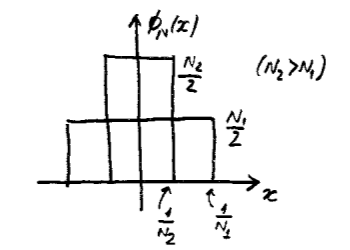
\includegraphics{figuras/08-0}
\end{figure}
% TODO Inserir número da página.
A série de Fourier dessa função já foi calculada (página ???, onde $a = 1 / N$)
tomando $L > 1 / N$, ou seja,
\begin{dmath*}
  \phi_N(x) = \frac{1}{2 L} + \sum_{n = 1}^{\infty} \left( \frac{N}{n \pi}
  \sin\left( \frac{n \pi}{N L} \right) \right) \cos\left( \frac{n \pi x}{L}
  \right).
\end{dmath*}

É fácil notarmos que à medida que aumentamos $N$, a função $\phi_N(x)$ fica cada
vez mais concentrada em torno de $x = 0$. A idéia intuitiva é que, para $N \to
\infty$, devemos ter
\begin{dmath*}
  \lim_{N \to \infty} \phi_N(x) = \begin{cases}
    +\infty, & x = 0, \\
    0, & x \neq 0.
  \end{cases}
\end{dmath*}
O problema, porém, é que não há sentido em definirmos uma função cujo valor em
um ponto seja $+\infty$. Também não temos como contornar esse problema
trabalhando com a série de Fourier pois ela não converge para $N \to \infty$, de
fato:
\begin{dmath*}
  \lim_{N \to \infty} \sum_{n = 1}^{\infty} \left( \frac{N}{n \pi} \sin\left(
  \frac{n \pi}{N L} \right) \right) \cos \left( \frac{n \pi x}{L} \right) =
  \sum_{n = 1}^{\infty} \frac{1}{L} \cos\left( \frac{n \pi x}{L} \right)
\end{dmath*}
que evidentemente não converge.

% TODO Inserir número da página.
Por outro lado, do teorema referente à integração da série de Fourier (página
???) sabemos que se $\phi_N(x)$ é contínua por partes, valoe a identidade
relacionada com a integração da série independentemente da série convergir ou
não. De fato:
\begin{dgroup*}
  \begin{dmath*}
    \int_{-L}^L \phi_N(x) \vi{x} = \int_{-1/N}^{1/N} N / 2 \vi{x}
    = (N / 2) (2 / N)
    = 1,
  \end{dmath*}
  \begin{dmath*}
    \int_{-L}^L \left( \frac{1}{2 L} + \sum_{n = 1}^{\infty}
    \frac{N}{n \pi} \sin\left( \frac{n \pi}{N L} \right) \cos\left(
    \frac{n \pi x}{L} \right) \right) = \frac{1}{2 L} 2 L + \sum_{n =
    1}^{\infty} \frac{N}{n \pi} \sin\left( \frac{n \pi}{N L} \right)
    \frac{L}{n \pi} \left. \sin\left( \frac{n \pi x}{L} \right) \right|_{-L}^L
    = \frac{1}{2 L} 2 L + \sum_{n = 1}^{\infty} \frac{N}{n \pi} \sin\left(
    \frac{n \pi}{N L} \right) \frac{L}{n \pi} 0
    = 1,
  \end{dmath*}
\end{dgroup*}
ou seja,
\begin{dmath*}
  \int_{-L}^L \phi_N(x) \vi{x} = \int_{-L}^L \left( \frac{1}{2 L} + \sum_{n =
  1}^{\infty} \frac{N}{n \pi} \sin\left( \frac{n \pi}{n L} \right) \cos\left(
  \frac{n \pi x}{L} \right) \right)
  = 1 \condition{$\forall N$}
\end{dmath*}
de modo que
\begin{dmath*}
  \lim_{N \to \infty} \int_{-L}^L \phi_N(x) \vi{x} = 1
\end{dmath*}
embora não exista $\lim_{N \to \infty} \phi_N(x)$.

Na verdade, podemos ir mais além. Seja $f(x)$ uma função que por enquanto basta
supor que possa ser representada por uma série de Fourier. Então:
\begin{dmath*}
  \int_{-L}^L f(x) \phi_N(x) \vi{x} = \int_{-L}^L \left( \frac{1}{2 L} + \sum_{n
  = 1}^{\infty} \frac{N}{n \pi} \sin\left( \frac{n \pi}{N L} \right) \cos\left(
  \frac{n \pi x}{L} \right)\right) f(x) \vi{x}
  = \frac{1}{2} \left[ \frac{1}{L} \int_{-L}^L f(x) \vi{x} \right] + \sum_{n =
  1}^{\infty} \frac{N L}{n \pi} \sin\left( \frac{n \pi}{N L} \right) \left[
  \frac{1}{L} \int_{-L}^L f(x) \cos\left( \frac{n \pi x}{L} \right) \right]
  = \frac{a_0}{2} + \sum_{n = 1}^{\infty} a_n \frac{N L}{n \pi} \sin\left(
  \frac{n \pi}{N L} \right)
\end{dmath*}
onde $a_0$ e $a_n$ são os coeficientes de Fourier de $f(x)$,
\begin{dmath*}
  f(x) = \frac{a_0}{2} + \sum_{n = 1}^{\infty} \left( a_n \cos\left(
  \frac{n \pi x}{L} \right) + b_n \sin\left( \frac{n \pi x}{L} \right) \right).
\end{dmath*}
Tomando $N \to \infty$,
\begin{dmath*}
  \lim_{N \to \infty} \int_{-L}^L f(x) \phi_N(x) \vi{x} = \frac{a_0}{2} +
  \sum_{n = 1}^{\infty} a_n
\end{dmath*}
que nada mais é do que $f(0)$,
\begin{dmath*}
  \lim_{N \to \infty} \int_{-L}^L f(x) \phi_N(x) \vi{x} = f(0)
\end{dmath*}
muito embora $\nexists \lim_{N \to \infty} \phi_N(x)$.

Na verdade, nós já nos deparamos com uma sitação análoga. Do Teorema de Fourier
e da expressão para o núcleo de Dirichlet, temos (considerando um período $T = 2
L$)
\begin{dmath*}
  f(x) = \lim_{N \to \infty} \int_{-L}^L f(\epsilon) D_N(\epsilon - x)
  \vi{\epsilon}
\end{dmath*}
onde
\begin{dmath*}
  D_N(x) = \frac{1}{2 L} \frac{\sin(N + 1/2) \pi x / L}{\sin(\pi x / (2 L))}.
\end{dmath*}
Como podemos ver $\nexists \lim_{N \to \infty} D_N(x)$ e mesmo assim
\begin{dgroup*}
  \begin{dmath*}
    \lim_{N \to \infty} \int_{-L}^L f(x) D_N(x) \vi{x} = f(0),
  \end{dmath*}
  \begin{dmath*}
    \lim_{N \to \infty} \int_{-L}^L D_N(x) \vi{x} = 1.
  \end{dmath*}
\end{dgroup*}
Temos, portanto, sequências que não convergem no sentido usual mas que, quando
tomadas dentro de uma integral com uma função $f(x)$, convergem para o mesmo
resultado, no caso $f(0$. Podemos pensar que essas sequências convergem (em um
outro sentido) para uma ``função'' $\delta(x)$ tal que $\int_{-L}^L \delta(x)
f(x) \vi{x} = f(0)$. Essa é a idéia que usaremos. Além disso, para aumentar a
classe de sequências que consideramos, vamos tomar $L \to \infty$, e para
assegurar que as integrais estejam bem definidas, vamos restringir o conjunto
das funções $f(x)$ que tomaremos nas integrais.

\section{Função Delta de Dirac}
\begin{defi}
  Uma função-teste é uma função infinitamente diferenciável tal que ela é
  identicamente nula fora de um intervalo finito $(a, b)$. Denotaremos o
  conjunto das funções-teste por $\mathcal{D}(R)$.
\end{defi}
\begin{exem}
  Um exemplo clássico de função-teste é
  \begin{dmath*}
    f(x) = \begin{cases}
      \exp(-1 / (1 - x^2), & \lvert x \rvert < 1, \\
      0, & \lvert x \rvert 1 \geq 1.
    \end{cases}
  \end{dmath*}
  Outros exemplos seguem quando notamos que se $f(x)$ é uma função-teste e
  $Q(x)$ é uma função infinitamente diferenciável, então $Q(x) f(x)$ é uma
  função-teste.
\end{exem}
\begin{defi}
  Uma sequência delta é uma sequência $\left\{ \phi_N(x) \right\}$ satisfazendo
  \begin{dmath*}
    \lim_{n \to \infty} \int_{-\infty}^{+\infty} \phi_n(x) \vi{x} = 1
  \end{dmath*}
  e, para $f(x) \in \mathcal{D}(R)$,
  \begin{dmath*}
    \lim_{n \to \infty} \int_{-\infty}^{+\infty} \phi_n(x) f(x) \vi{x} = f(0).
  \end{dmath*}
  Definimos a função delta de Dirac como sendo o limite de uma sequência delta,
  onde esse limite é interpretado no sentido de
  \begin{dmath*}
    \int_{-\infty}^{+\infty} \delta(x) f(x) \vi{x} = \lim_{n \to \infty}
    \int_{-\infty}^{+\infty} \phi_n(x) f(x) \vi{x}.
  \end{dmath*}
  Assim sendo, a função delta de Dirac satisfaz
  \begin{dmath*}
    \int_{-\infty}^{+\infty} \phi_(x) f(x) \vi{x} = f(0).
  \end{dmath*}
  Evidentemente $\delta(x)$ não é uma ``função'' no sentido usual. Ela é o que
  chamamos uma ``função generalizada'' ou ``distribuição''.
\end{defi}
\begin{exem}
  Exemplos de sequência delta, além daquelas da seção anterior, são:
  \begin{enumerate}
    \item $\phi_n(x) = (n / \pi) (1 / (1 + n^2 x^2))$,
    \item $\phi_n(x) = (n / \sqrt{\pi}) \exp(-n^2 x^2)$,
    \item $\phi_n(x) = 1 / (n \pi) (\sin^2(n x) / x^2)$,
    \item $\phi_n(x) = n J_n(n (1 + x))$,
    \item $\phi_n(x) = n \exp(-n x^2) L_k(2 n x)$,
  \end{enumerate}
  onde $J_n(x)$ é a função de Bessel de ordem $n$ e $L_k(x)$ é o polinômio de
  Laguere de ordem $k$ (arbitrário).
\end{exem}

Podemos ainda definir a função delta transladada $\delta(x - a)$. Nesse caso:
\begin{dmath*}
  \int_{-\infty}^{+\infty} \delta(x - a) f(x) \vi{x} = f(a).
\end{dmath*}
Para vermos isso usamos a definição via sequência delta:
\begin{dmath*}
  \int_{-\infty}^{+\infty} \delta(x - a) f(x) \vi{x} = \lim_{n \to \infty}
  \int_{-\infty}^{+\infty} \phi_n(x - a) f(x) \vi{x}
  = \lim_{n \to \infty} \int_{-\infty}^{+\infty} \phi_n(y) f(y + a) \vi{y}
  = \int_{-\infty}^{+\infty} \delta(y) f(y + a) \vi{y}
  = f(a).
\end{dmath*}
Isso, aliás, mostra que podemos fazer mudanças de variáveis diretamente dentro
da integral com a função delta. Dessa forma podemos mostrar por exemplo, que
para $a \neq 0$
\begin{dmath*}
  \delta(a x) = \delta(x) / \lvert a \rvert.
\end{dmath*}
De fato, se $a > 0$:
\begin{dmath*}
  \int_{-\infty}^{+\infty} \delta(a x) f(x) \vi{x} = \int_{-\infty}^{+\infty}
  \delta(y) f(y / a) \frac{\vi{y}}{a}
  = \frac{f(0)}{a}
  = \int_{-\infty}^{+\infty} \frac{\delta(x)}{\lvert a \rvert} f(x) \vi{x}
\end{dmath*}
enquanto, se $a < 0$:
\begin{dmath*}
  \int_{-\infty}^{+\infty} \delta(a x) f(x) \vi{x} = \int_{+\infty}^{-\infty}
  \delta(y) f(y / a) \frac{\vi{y}}{a}
  = -\frac{f(0)}{a}
  = \int_{-\infty}^{+\infty} \frac{\delta(x)}{\lvert a \rvert} f(x) \vi{x}.
\end{dmath*}

Já com um pouco mais de engenhosidade, podemos mostrar que, para $a \neq 0$:
\begin{dmath*}
  \delta(x^2 - a^2) = \frac{1}{2 \lvert a \rvert} \left[ \delta(x + a) +
  \delta(x - a) \right].
\end{dmath*}
Para isso vamos considerar as funções-teste que são identicamente nulas fora do
intervalo $(-a , a)$. Vamos denotar esse conjunto por $\mathcal{D}(-a, a)$, de
mode que $\mathcal{D}(-a, a) \subset \mathcal{D}(R)$. Tomando $x^2  - a^2 = y$,
temos que para $x \geq 0$, $x = \sqrt{y - a^2}$, $y - a^2 \leq y < \infty$,
enquanto para $x \leq 0$, $x = -\sqrt{y + a^2}$, $-a^2 \leq y < \infty$. Logo
\begin{dmath*}
  \int_{-\infty}^{+\infty} \delta(x^2 - a^2) f(x) \vi{x} = \int_{-\infty}^0
  \delta(x^2 - a^2) f(x) \vi{x} + \int_0^{\infty} \delta(x^2 - a^2) f(x) \vi{x}
  = \int_{-\infty}^{-a^2} \delta(y) f(-\sqrt{y + a^2}) \frac{- \vi{y}}{2 \sqrt{y
  + a^2}} + \int_{-a^2}^{\infty} \delta(y) f(\sqrt{y + a^2})
  \frac{\vi{y}}{2 \sqrt{y + a^2}}
  = \frac{f(-\sqrt{a^2})}{2\sqrt{a^2}} + \frac{f(\sqrt{a^2})}{2 \sqrt{a^2}}
  = \frac{1}{2 \lvert a \rvert} \int_{-\infty}^{+\infty} \left[ \delta(x + a) +
  \delta(x - a) \right] f(x) \vi{x},
\end{dmath*}
onde usamos que $f(x) \in \mathcal{D}(-a, a)$. Portanto $\delta(x^2 - a^2)$ age
sobre $f \in \mathcal{D}(-a, a)$ de uma forma tal que é a mesma que $1 / (2
\lvert a \rvert) \left[ \delta(x + a) + \delta(x - a) \right]$ agindo sobre $f
\in \mathcal{D}(R)$.

Dentro do cálculo com a função delta, é natural procurarmos definir a derivada
$\delta'(a)$. Se $\left\{ \phi_n(x) \right\}$ é uma sequência delta, definimos
$\delta'(a)$ como a distribuição associada com as derivadas dessa sequência, ou
seja,
\begin{dmath*}
  \int_{-\infty}^{+\infty} \delta'(x) f(x) \vi{x} = \lim_{n \to \infty}
  \int_{-\infty}^{+\infty} \phi'_n(x) f(x) \vi{x},
\end{dmath*}
onde $f \in \mathcal{D}(R)$. Mas, integrando por partes
\begin{dmath*}
  \int_{-\infty}^{+\infty} \phi'_n(x) f(x0 \vi{x} = \left. \phi_n(x) f(x)
  \right|_{-\infty}^{+\infty} - \int_{-\infty}^{+\infty} \phi_n(x) f'(x) \vi{x}
\end{dmath*}
e como $f(x) \equiv 0$ para $x \notin (a, b)$, de modo que $\lim_{x \to
\pm\infty} f(x) = 0$,
\begin{dmath*}
  \left. \phi_n(x) f(x) \right|_{-\infty}^{+\infty} = 0
\end{dmath*}
e portanto
\begin{dmath*}
  lim_{n \to \infty} \int_{-\infty}^{+\infty} \phi'_n(x) f(x) \vi{x} = -\lim_{n
  \to \infty} \int_{-\infty}^{+\infty} \phi_n(x) f'(x) \vi{x}
  = -\int_{-\infty}^{+\infty} \delta(x) f'(x) \vi{x}
  = -f'(0).
\end{dmath*}
Portanto,
\begin{dmath*}
  \int_{-\infty}^{+\infty} \delta'(x) f(x) \vi{x} = -f'(0).
\end{dmath*}

A derivada $n$-ésima $d^{(n)}(x)$ é definida de forma análoga. Repetindo os
passos aacima, lembranddo que $f^{(k)}(x) \equiv 0$ para $x \notin (a, b)$ e $k
= 0, 1, 2, \ldots$, segue que
\begin{dmath*}
  \int_{-\infty}^{+\infty} \delta^{(n)}(x) f(x) \vi{x} = (-1)^n f^{(n)}(0).
\end{dmath*}

Podemos ainda nos perguntar pela primiteva da função delta, ou seja, uma
distribuição $H(x)$ tal que $\delta(x) = H'(x)$. A definição natural é
\begin{dmath*}
  \int_{-\infty}^{+\infty} H(x) f(x) \vi{x} = \lim_{n \to \infty}
  \int_{-\infty}^{+\infty} \Phi_n(x) f(x) \vi{x}
\end{dmath*}
onde $\Phi_n(x)$ é uma primitiva de $\phi_n(x)$, por exemplo:
\begin{dmath*}
  \Phi_n(x) = \int_{-\infty}^x \phi_n(x)(\epsilon) \vi{\epsilon}.
\end{dmath*}
Com isso e trocando a ordem de integração
\begin{dmath*}
  \int_{-\infty}^{+\infty} \Phi_n(x) f(x) \vi{x} = \int_{-\infty}^{+\infty}
  \left[ \int_{-\infty}^x \phi_n(\epsilon) \vi{\epsilon} \right] f(x) \vi{x}
  = \int_{-\infty}^{+\infty} \left[ \int_{\epsilon}^{+\infty} f(x) \vi{x}
  \right] \phi_n(\epsilon) \vi{\epsilon}
\end{dmath*}
e como isso
\begin{dmath*}
  \lim_{n \to \infty} \int_{-\infty}^{+\infty} \Phi_n(x) f(x) \vi{x} = \lim_{n
  \to \infty} \int_{-\infty}^{+\infty} \phi_n(\epsilon) \left[
  \int_{\epsilon}^{+\infty} f(x) \vi{x} \right] \vi{\epsilon}
  = \int_{-\infty}^{+\infty} \delta(\epsilon) \left[ \int_{\epsilon}^{+\infty}
  f(x) \vi{x} \right] \vi{\epsilon}
  = \int_0 {\infty} f(x) \vi{x},
\end{dmath*}
ou seja,
\begin{dmath*}
  \int_{-\infty}^{+\infty} H(x) f(x) \vi{x} = \int_0^{\infty} f(x) \vi{x}
\end{dmath*}
de modo que
\begin{dmath*}
  H(x) = \begin{cases}
    1, & x > 0, \\
    0, & x < 0,
  \end{cases}
\end{dmath*}
que é a chamada função escada ou de Heaviside.

\begin{exem}
  As seguintes sequência convergem (no sentido de $\lim_{n \to \infty}
  \int_{-\infty}^{+\infty} \Phi_n(x) f(x) \vi{x} = \int_{-\infty}^{+\infty} H(x)
  f(x) \vi{x})$) para a função escada:
  \begin{itemize}
    \item $\Phi_n(x) = (1 / 2) \operatorname{erfc}(-n x) = (1 / \sqrt{\pi})
      \int_{-n x}^{\infty} \exp(-u^2) \vi{u}$,
    \item $\Phi_n(x) = (1 / 2) + (1 / \pi) \sin(n x) = (1 / \pi)
      \int_{-\infty}^{n x} \sin(u) / u \vi{u}$,
    \item $\Phi_n(x) = \exp(- \exp(n x))$.
  \end{itemize}
\end{exem}

% 'Notas de aula não oficiais de MS650 e F620' (c) 2012, 2013 by Raniere Silva
% <ra092767@ime.unicamp.br>
%
% 'Notas de aula não oficiais de MS650 e F620' is licensed under a
% Creative Commons Attribution-ShareAlike 3.0 Unported License.
%
% You should have received a copy of the license along with this
% work.  If not, see <http://creativecommons.org/licenses/by-sa/3.0/>.

% Este arquivo inclui o conteúdo de:
%
% * M2S12-9.pdf
% * M2S12-10.pdf
% * M2S12-11.pdf
% * M2S12-12.pdf

\chapter{Transformadas de Fourier}
\subsection{Da série para a Transformada}
Seja a série de Fourier de uma função com período $T = 2L$,
\begin{align*}
    f(x) &= \sum_{n = -\infty}^\infty c_n \exp\left( i n \pi x / L \right), \\
    c_n &= \frac{1}{2L} \int_{-L}^L f(x) \exp\left( -i n \pi x / L \right)
    \id{x}.
\end{align*}
O que desejamos agora é considerar uma função que não seja
necessariamente periódica, ou seja, estender o intervalo para todo o
$\mathbb{R}$ tomando $L \to \infty$. Para isso vamos denotar
\begin{align*}
    K = K(n) &= n \pi / L, \\
    \Delta K &= K(n + 1) - K(n) = \pi / L.
\end{align*}
Então:
\begin{align*}
    f(x) &= \sum_{n = -\infty}^\infty c_n \exp\left( i K(n) x \right) \\
    &= \sum_{n = -\infty}^\infty \left( \frac{c_n L}{\pi} \right) \exp\left(
    i K(n) x \right) \Delta K
\end{align*}
com
\begin{align*}
    \frac{c_n L}{\pi} &= \frac{1}{2 \pi} \int_{-\infty}^\infty f(x) \exp\left(
    -i K(n) x \right) \id{x}.
\end{align*}

Vamos agora pensar em $n$ como uma função de $K$, ou seja, $n = n(K) = K
L / \pi$. Então
\begin{align*}
    \frac{c_n L}{\pi} &= c_{K L / \pi} L / \pi = c_L(K)
\end{align*}
e
\begin{align*}
    f(x) &= \sum_{K L / \pi = -\infty}^\infty c_L(K) \exp\left( i K x \right)
    \Delta K, \\
    c_L(K) &= \frac{1}{2 \pi} \int_{-L}^L f(x) \exp\left( - i K x \right)
    \id{x}.
\end{align*}
Agora, uma vez que $\Delta K L / \pi = 1$, para $L \to \infty$ temos $\Delta K
\to 0$ e a soma acima torna-se uma integral de Riemann. Portanto, para $L \to
\infty$:
\begin{align*}
    f(x) &= \int_{-\infty}^\infty c(K) \exp\left( i K x \right) \id{K},
    c(K) &= \frac{1}{2 \pi} \int_{-\infty}^\infty f(x) \exp\left( - i K x
    \right) \id{x}.
\end{align*}
Finalmente, para tornar essas expressões ``simétricas'', vamos definir
$F(K) = \sqrt{2 \pi} c(-K)$. Assim
\begin{align*}
    f(x) &= \frac{1}{\sqrt{2 \pi}} \int_{-\infty}^\infty F(K) \exp\left( -i K x
    \right) \id{K}, \\
    F(K) &= \frac{1}{\sqrt{2 \pi}} \int_{-\infty}^\infty f(x) \exp\left( i K x
    \right) \id{x},
\end{align*}
onde $F(K)$ é a transformada de Fourier de $f(x)$, $f(x)$ é a
transformada de Fourier inversa de $F(K)$, $F(K) = \mathcal{F}\left\{ f(x)
\right\}$ e $f(x) = \mathcal{F}^{-1}\left\{ F(K) \right\}$.
\begin{exem}
    Considere $f(x) = N \exp\left( - \alpha x^2 \right)$ para $\alpha > 0$.
    % TODO Terminar de incluir exemplo da página 115.
\end{exem}
\begin{exem}
    Considere $f(x) = a / \left( x^2 + a^2 \right)$ para $a > 0$.
    % TODO Terminar de incluir exemplo da página 116.
\end{exem}
\begin{exem}
    Considere
    \begin{align*}
        f(x) &= \begin{cases}
            1, & |x| \leq a, \\
            0, & |x| > a,
        \end{cases}
    \end{align*}
    para $a > 0$.
    % TODO Terminar de incluir exemplo da página 117.
\end{exem}
\begin{exem}
    Considere $f(x) = \delta(x)$.
    % TODO Terminar de incluir exemplo da página 117.
\end{exem}

\section{Fórmula Integral de Fourier}
Na página~\pageref{teo:fourier} estudamos o Teorema de Fourier para
séries. Considerando um período $T = 2L$, esse teorema garante que a
série
\begin{align*}
    f(x) &= \frac{1}{2L} \int_{-L}^L f(\xi) \id{\xi} + \frac{1}{L} \sum_{n =
    1}^\infty \int_{-L}^L f(\xi) \cos\left( n \pi (\xi - x) / L \right) \id{\xi}
    \\
    &= \lim_{N \to \infty} \int_{-L}^L f(x) \frac{\sin\left( (N + 1 / 2) \pi
    (\xi - x) / L \right)}{2 L \sin\left( \pi (\xi - x) / 2 L \right)}
\end{align*}
quando $f(x)$ é contínua por partes e com derivadas laterais em $(-L,
L)$ e com período $2L$.

Vamos agora considerar o limite $L \to \infty$. Para isso vamos supor que exista
a integral
\begin{align*}
    \int_{-\infty}^\infty |f(x)| \id{x} < \infty.
\end{align*}
Nesse caso, temos
\begin{align*}
    \lim_{L \to \infty} \frac{1}{2L} \int_{-\infty}^\infty f(\xi) \id{\xi} = 0
\end{align*}
e agora devemos ver o que acontece com a série.

Definindo, como na seção anterior,
\begin{align*}
    K &= N \pi / L, \\
    \Delta K &= \pi / L
\end{align*}
temos
\begin{align*}
    \frac{1}{L} \sum_{n = 1}^\infty \int_{-L}^L f(\xi) \cos\left( n \pi (\xi -
    x) / L \right) \id{\xi} &= \frac{1}{\pi} \sum_{n = 1}^\infty \Delta K
    \int_{-L}^L f(\xi) \cos\left( K(\xi - x) \right) \id{\xi}.
\end{align*}
Para $L \to \infty$ temos $\Delta K \to 0$ e a soma pode ser tomada por uma
integral de Riemann de $K = 0$ até $K = \infty$ (pois $K = 0$ para $L \to
\infty$ e $n$ fixo). Logo:
\begin{align*}
    f(x) &= \frac{1}{\pi} \int_0^\infty \int_{-\infty}^\infty f(\xi) \cos\left(
    K(\xi - x) \right) \id{\xi} \id{K}.
\end{align*}
Essa é a fórmula de Fourier. Apesar da natureza heurística as
argumentações acima, iremos mostrar agora que ela é de fato
válida. Para isso precisamremos estender o Lema~\ref{lem:lim_int} da
página~\pageref{lem:lim_int} de modo a incluir a integral ao longo de toda a
reta, ou seja, precisamos do seguinte:
\begin{lem}
    Seja $F$ uma função contínua por partes e com derivadas lateria
    \`{a} esquerda e \`{a} direita para todo o intervalo real tal que exista a
    integral $\int_{-\infty}^\infty |F(x)| \id{x} < \infty$. Então
    \begin{align*}
        \lim_{k \to \infty} \int_{-\infty}^\infty F(x) \frac{\sin\left( K(x -
        x_0)
        \right)}{ x - x_0} \id{x} &= \pi \frac{F(x_0 + 0) + F(x_0 - 0)}{2}.
    \end{align*}
\end{lem}
\begin{proof}
    Vamos denotar
    \begin{align*}
        G(x, x_0; K) &= F(x) \frac{\sin\left( k (x - x_0) \right)}{x - x_0} \\
        &= K F(x) \frac{\sin(K (x - x_0)}{K (x - x_0)} \\
        &= K F(x) S\left( K(x - x_0) \right).
    \end{align*}
    Vimos durante a demonstração do Lema~\ref{lem:cont}
    (página~\pageref{lem:cont}) que $|S(x)| \leq 1$ para $x \in \mathbb{R}$;
    logo:
    \begin{align*}
        |G(x, x_0; K) \leq K|F(x)|
    \end{align*}
    e
    \begin{align*}
        \int_{-\infty}^\infty |G(x, x_0; K) \id{x} \leq K \int_{-\infty}^\infty
        |F(x)| \id{x} < \infty
    \end{align*}
    de modo que existe a integral $\int_{-\infty}^\infty G(x, x_0; K) \id{x}.$
    Seja
    \begin{align*}
        H(x_0; K) &= \int_{-\infty}^\infty G(x, x_0; K) \id{x} -
        \frac{\pi}{2} \left[ F(x_0 + 0) + F(x_0 - 0) \right].
    \end{align*}
    % TODO Terminar a demonstração a partir da página 123.
\end{proof}

Agora podemos provar o seguinte:
\begin{teo}
    Seja $f(x)$ contínua por partes e com derivadas laterais \`{a} esquerda
    e \`{a} direita em todo intervalo real tal que $\int_{-\infty}^\infty |f(x)|
    < \infty$. Então vale a chamada fórmula integral de  Fourier:
    \begin{align*}
        \frac{1}{\pi} \int_0^\infty \int_{-\infty}^\infty f(\xi) \cos\left(
        K(\xi - x) \right) \id{\xi} \id{K} &= \frac{1}{2} \left[ f(x + 0) + f(x
        - 0) \right]
    \end{align*}
    para $-\infty < x < \infty$.
\end{teo}
\begin{proof}
    % TODO Terminar a demonstração a partir da página 125.
\end{proof}

Vamos agora escrever a fórmula integral de Fourier de uma outra forma.
Usando $\cos(\phi) = \left( \exp(i \phi) + \exp(-i \phi) \right) / 2$,
\begin{align*}
    I &= \frac{1}{2} \left[ f(x + 0) + f(x - 0) \right] \\
    &= \frac{1}{\pi} \lim_{a \to \infty} \int_0^a \int_{-\infty}^\infty f(\xi)
    \left[ \frac{\exp\left( i K(\xi - x) \right) + \exp\left( - i K(\xi - x)
    \right)}{2} \right]
    % Terminar de digitar equações.
\end{align*}
o que mostra que na transformada inversa a integral deve ser interpretada no
sentido do valor principal de Cauchy:
\begin{align*}
    \mathcal{F}^{-1}\left[ F(K) \right] &= \frac{1}{\sqrt{2 \pi}} PV
    \int_{-\infty}^\infty F(K) \exp\left( -i K x \right) \id{x} \\
    &= \frac{1}{\sqrt{2 \pi}} \lim_{a \to \infty} \int_{-a}^a F(k) \exp\left(
    -i K x \right) \id{K}.
\end{align*}
\begin{exem}
    Considerando
    \begin{align*}
        f(x) &= \begin{cases}
            0, & x < 0, \\
            \exp\left( -x \right), & x > 0.
        \end{cases}
    \end{align*}
    % TODO Terminar a demonstração a partir da página 127.
\end{exem}

\section{Propriedades das Transformadas de Fourier}
Notação: $F(K) = \mathcal{F}\left[ f(x) \right]$.

\subsection{Translação}
Temos que
\begin{align*}
    \mathcal{F}\left[ f(x - a) \right] &= \exp\left( i K a \right) F(K), \\
    \mathcal{F}\left[ \exp\left( -i \alpha x \right) f(x) \right] &= F(k -
    \alpha),
\end{align*}
portanto, a translação em um espaço equivale \`{a}
multiplicação por uma exponencial (complexa) no espaço
recíproco.
\begin{proof}
    \begin{align*}
        \mathcal{F}\left[ f(x - a) \right] &= \frac{1}{\sqrt{2 \pi}}
        \int_{-\infty}^\infty f(x - a) \exp\left( i K x \right) \id{x} \\
        &= \frac{1}{\sqrt{2 \pi}} \int_{-\infty}^\infty f(x') \exp\left( i K(x'
        + a) \right) \id{x} \\
        &= \exp\left( i K a \right) F(K), \\ \mathcal{F}\left[ \exp\left( -i
        \alpha x \right) f(x) \right] &= \frac{1}{\sqrt{2 \pi}}
        \int_{-\infty}^\infty f(x) \exp\left( -i \alpha x \right) \exp\left( i K
        x \right) \id{x} \\
        &= \frac{1}{\sqrt{2 \pi}} \int_{-\infty}^\infty f(x) \exp\left( i (k -
        \alpha) x \right) \id{x} \\
        &= F(k - \alpha).
    \end{align*}
\end{proof}

\subsection{Derivação}
Temos que
\begin{align*}
    \mathcal{F}\left[ f'(x) \right] &= -i K F(K), \\
    \mathcal{F}\left[ x f(x) \right] &= -i F'(K),
\end{align*}
portanto, a derivação em relação \`{a} uma variável equivale
\`{a} ultiplicação pela outra variável do espaço recíproco.
\begin{proof}
    % TODO Terminar a demonstração a partir da página 130.
\end{proof}

A generalização dessas propriedades é óbvia:
\begin{align*}
    \mathcal{F}\left[ f^{(n)}(x) \right] &= (-i K)^n F(K), \\
    \mathcal{F}\left[ x^n f(x) \right] &= (-i)^n F^{(n)}(K),
\end{align*}
onde em $\mathcal{F}\left[ f^{(n)}(x) \right]$ devemos upor $\lim_{x \to
\pm\infty} f^{(k)}(x) = 0$ para $k = 0, 1, \ldots, n - 1$.
\begin{obs}
    É interessante notarmos que as propriedades de translação e
    derivação se unem através do Teorema de Taylor; de fato,
    escrevendo $f(x - a)$ na forma de uma série de Taylor em torno de $x =
    a$,
    \begin{align*}
        f(x - a) &= \sum_{n = 0}^\infty \frac{f^{(n)}(x)}{n!}(-a)^n
    \end{align*}
    segue, da linearidade de $\mathcal{F}$,
    \begin{align*}
        \mathcal{F}\left[ f(x - a) \right] &= \sum_{n = 0}^\infty
        \frac{(-a)^n}{n!} \mathcal{F}\left [f^{(n)}(x) \right] \\
        &= \sum_{n = 0}^\infty \frac{(-a)^n (-iK)^n}{n!} F(K) \\
        &= \sum_{n = 0}^\infty \frac{(i K a)^n}{n!} F(K) \\
        &= \exp\left( i K a \right) F(K).
    \end{align*}
\end{obs}

\subsection{Identidade de Parseval}
Temos que
\begin{align*}
    \int_{-\infty}^\infty f(x) g^K(x) \id{x} &= \int_{-\infty}^\infty F(K)
    G^K(K) \id{K}.
\end{align*}
\begin{proof}
    % TODO Terminar a demonstração a partir da página 131.
\end{proof}
Uma consequência muito importante desse resultado é:
\begin{align*}
    \int_{-\infty}^\infty |f(x)|^2 \id{x} &= \int_{-\infty}^\infty |F(K)|^2
    \id{K}.
\end{align*}
sendo essa identidade também chamada identidade de Parseval. Dessa forma, em
outras palavras:
\begin{align*}
    \| f \|^2 = \| F \|^2.
\end{align*}

\subsection{Teorema da Convolução}
% TODO Terminar de incluir arquivo M2S12-10.pdf. Interrompido na página 132.

\section{Aplicações da transformada de Fourier na solução de Equações
Diferenciais}
\begin{exem}
  Considere a equação do oscilador harmônico amortecido
  \begin{dmath*}
    \fder{^2 x}{t^2} + 2 \alpha \fder{x}{t} + w_0^2 x = f(t),
  \end{dmath*}
  onde $\alpha > 0$, $w_0^2 = k / m$ e $f(t) = F(t) / m$.

  Então,
  % TODO concluir o exemplo. M212-11.pdf
\end{exem}

\begin{exem}
  Considere a equação da onda
  \begin{dmath*}
    \pder{^2 u}{x^2} = \frac{1}{v^2} \pder{^2 u}{t^2},
  \end{dmath*}
  onde $-\infty < x < \infty$.

  Então,
  % TODO concluir o exemplo. M212-11.pdf
\end{exem}

\section{Transformadas em seno e cosseno de Fourier}
Considerando
\begin{dmath*}
  \mathcal{F}[f(x)] = \frac{1}{\sqrt{2 \pi}} \int_{-\infty}^{\infty} f(x) \exp(i
  k x) \vi{x}
  = \frac{1}{\sqrt{2 \pi}} \int_{-\infty}^0 f(x) \exp(i k x) \vi{x} +
  \frac{1}{\sqrt{2 \pi}} \int_0^{+\infty} f(x) \exp(i k x) \vi{x}
  = \frac{1}{\sqrt{2 \pi}} \int_0^{\infty} f(-x) \exp(-i k x) \vi{x} +
  \frac{1}{\sqrt{2 \pi}} \int_0^{+\infty} f(x) \exp(i k x) \vi{x}.
\end{dmath*}
Para $f(x)$ uma função par temos
\begin{dmath*}
  \mathcal{F}[f(x)] = \frac{1}{\sqrt{2 \pi}} \int_0^{\infty} f(x) \exp(-i k x)
  \vi{x} + \frac{1}{\sqrt{2 \pi}} \int_0^{\infty} f(x) \exp(i k x) \vi{x}
  = \frac{2}{\sqrt{2 \pi}} \int_0^{\infty} f(x) \left[ \frac{\exp(i k x) +
  \exp(-i kx)}{2} \right]
  = \sqrt{\frac{2}{\pi}} \int_0^{\infty} f(x) \cos(k x) \vi{x}
  = \mathcal{F}_C[f(x)]
  = \mathcal{F}_C(k).
\end{dmath*}
Logo, a transformada de cossenos de Fourier é
\begin{dmath*}
  \mathcal{F}_c(k) \hiderel{=} \mathcal{F}_c[f(x)] = \sqrt{\frac{2}{\pi}}
  \int_0^{\infty} f(x) \cos(k x) \vi{x}.
\end{dmath*}
Como $\cos(k x)$ é par, é imediato que $\mathcal{F}_c(k)$ é par. Logo, repetindo
o raciocínio acima para $\mathcal{F}^{-1}[F_c(k)]$ vamos encontar que
$\mathcal{F}^{-1}[F_c(k)] = \mathcal{F}^{-1}[F_c(k)]$, onde
\begin{dmath*}
  f(x) = \mathcal{F}^{-1}_c[F_c(k)]
  = \sqrt{\frac{2}{\pi}} \int_0^{\infty} F_c(k) \cos(k x) \vi{k}
\end{dmath*}
é a transformada inversa em cossenos de Fourier.

Para $f(x)$ ímpar temos que
\begin{dmath*}
  \mathcal{F}[f(x)] = \frac{-1}{\sqrt{2 \pi}} \int_0^{\infty} f(x) \exp(-i k x)
  \vi{x} + \frac{1}{\sqrt{2 \pi}} \int_0^{\infty} f(x) \exp(i k x) \vi{x}
  = \frac{2 i}{\sqrt{2 \pi}} \int_0^{\infty} f(x) \left[ \frac{\exp(i k x) -
  \exp(-i k x)}{2 i} \right] \vi{x}
  = i \sqrt{\frac{2}{\pi}} \int_0^{\infty} f(x) \sin(k x) \vi{x}
  = i \mathcal{F}_s[f(x)]
  = i F_s(k).
\end{dmath*}
Logo, a transformada de seno de Fourier é
\begin{dmath*}
  F_s(k) \hiderel{=} \mathcal{F}_s[f(s)] = \sqrt{\frac{2}{\pi}} \int_0^{\infty}
  f(x) \sin(k x) \vi{x}.
\end{dmath*}
Como $\sin(k x)$ é ímpar, segue que $F_s(k)$ é ímpar. Logo,
\begin{dmath*}
  f(x) = \mathcal{F}^{-1}[F(k)]
  = i \mathcal{F}^{-1}[F_s(k)]
  = i \frac{1}{\sqrt{2 \pi}} \int_{-\infty}^{+\infty} F_s(k) \exp(-i k x) \vi{k}
  = i \frac{1}{\sqrt{2 \pi}} \left[ \int_{-\infty}^0 F_s(k) \exp(-i k x) \vi{k}
  + \int_0^{\infty} F_s(k) \exp(-i k x) \vi{k} \right]
  = i \frac{1}{\sqrt{2 \pi}} \left[ \int_0^{\infty} F_s(k) \exp(i k x) \vi{k} +
  \int_0^{\infty} F_s(k) \exp(-i k x) \vi{k} \right]
  = \frac{2}{\sqrt{2 \pi}} \int_0^{\infty} \left[ \frac{\exp(i k x) - \exp(-i k
  x)}{2 i} \right] F_s(k) \vi{k}
  = \sqrt{\frac{2}{\pi}} \int_0^{\infty} F_s(k) \sin(k x) \vi{k}.
\end{dmath*}
Portanto, a transformada inversa em seno de Fourier é
\begin{dmath*}
  f(x) \hiderel{=} \mathcal{F}_s^{-1}[F_s(k)] = \sqrt{\frac{2}{\pi}}
  \int_0^{\infty} F_s(k) \sin(k x) \vi{k}.
\end{dmath*}

\begin{obs}
  Um dos aspectos negativos das transformadas em seno e em cosseno é a perda da
  dualidade existente na transformada de Fourier. Por exemplo, já não vale a
  propriedade que derivar em um espaço equivale a multiplicação pela variável do
  espaço recíproco. De fato, supondo $\lim_{x \to \infty} f(x) = 0$, podemos ver
  facilmente através de integração por partes que
  \begin{dgroup*}
    \begin{dmath*}
      \mathcal{F}_c[f'(x)] = -\sqrt{2 / \pi} f(0) + k \mathcal{F}_s[f(x)]
    \end{dmath*}
    \begin{dmath*}
      \mathcal{F}_s[f'(x)] = -k \mathcal{F}_c[f(x)]
    \end{dmath*}
  \end{dgroup*}

  Além disso, não é imediato como podemos relacionar as transformadas em seno e
  cosseno das funções $f(x)$ e $f(x - a)$ pois no primeiro caso só consideramos
  os valores de $f(s)$ para $s > 0$ enquanto no segundo devemos considerar os
  valores de $f(s)$ para $s > -a$.

  Já quanto à convolução, podemos notar que a inversão do produto $F_c(k)
  G_c(k)$, onde $F_c(k) = F_c[f(x)]$ e $G_c(k) = F_c[g(x)]$, se faz através de
  $\mathcal{F}^{-1}$ pois o produto de duas funções pares é uma função par. Por
  outro lado, o produto de duas funções ímpares é uma função par. Logo, a
  inversão de $F_s(k) G_s(k)$ deve ser feita usando $\mathcal{F}_c^{-1}$. Com
  isso:
  \begin{dgroup}
    \begin{dmath*}
      \mathcal{F}_c^{-1}[F_c(k) G_c(k)] = \sqrt{\frac{2}{\pi}} \int_0^{\infty}
      F_c(k) G_c(k) \cos(k x) \vi{k}
      = \sqrt{\frac{2}{\pi}} \int_0^{\infty} F_c(k) \sqrt{\frac{2}{\pi}}
      \int_0^{\infty} g(\epsilon) \cos(k \epsilon) \cos(k x) \vi{\epsilon} \vi{k}
      = \frac{1}{\pi} \int_0^{\infty} g(\epsilon) \int_0^{\infty} F_c(k) \cos(k (x
      - \epsilon)) \vi{k} \vi{\epsilon} + \frac{1}{\pi} \int_0^{\infty}
      g(\epsilon) \int_0^{\infty} F_c(k) \cos(k (x + \epsilon)) \vi{k}
      \vi{\epsilon}
      = \frac{1}{\sqrt{2 \pi}} \int_0^{\infty} g(\epsilon) f(x - \epsilon)
      \vi{\epsilon} + \frac{1}{\sqrt{2 \pi}} \int_0^{\infty} g(\epsilon) f(x +
      \epsilon) \vi{\epsilon},
    \end{dmath*}
    \begin{dmath*}
      \mathcal{F}_c^{-1}[F_s(k) G_s(k)] = \sqrt{\frac{2}{\pi}} \int_0^{\infty}
      F_s(k) G_s(k) \cos(k x) \vi{k}
      = \sqrt{\frac{2}{\pi}} \int_0^{\infty} F_s(k) \sqrt{\frac{2}{\pi}}
      \int_0^{\infty} g(\epsilon) \sin(k \epsilon) \cos(k x) \vi{\epsilon}
      \vi{k}
      = \frac{1}{\pi} \int_0^{\infty} g(\epsilon) \int_0^{\infty} F_s(k) \sin(k
      (\epsilon - x)) \vi{k} \vi{\epsilon} + \frac{1}{\pi} \int_0^{\infty}
      g(\epsilon) \int_0^{\infty} F_s(k) sin(k (\epsilon + x)) \vi{k}
      \vi{\epsilon}
      = \frac{1}{\sqrt{2 \pi}} \int_0^{\infty} g(\epsilon) f(\epsilon - x)
      \vi{\epsilon} + \frac{1}{\sqrt{2 \pi}} \int_0^{\infty} g(\epsilon)
      f(\epsilon + x) \vi{\epsilon}.
    \end{dmath*}
  \end{dgroup}

  Isso tudo mostra que as transformadas em seno e cosseno não são tão ``boa''
  quando a transformada de Fourier. Veremos, entretando, que quando consideramos
  apenas o intervalo $0 \leq x \leq \infty$, existe uma melhor opção que as
  transformadas em seno e cosseno que é a transformada de Laplace.
\end{obs}

\begin{exem}
  Considere o sistema
  \begin{dmath*}
    \begin{cases}
      \fder{^2 x}{t^2} - \alpha^2 x = 0, & 0 \leq t \leq \infty, \\
      \fder{x}{t}(0) = b, \\
      \lim_{t \to \infty} x(t) = 0.
    \end{cases}
  \end{dmath*}
  Vamos usar a transformada em cossenos para resolver esse problema.
  \begin{dmath*}
    \mathcal{F}_c\left[ \fder{^2 x}{t^2} \right] = - \sqrt{\frac{2}{\pi}}
    \fder{x}{t}(0) + k \mathcal{F}_s\left[ \fder{x}{t} \right]
    = \sqrt{\frac{2}{\pi}} b + k \left( -k \mathcal{F}_c[x] \right)
    = -b \sqrt{\frac{2}{\pi}} - k^2 \mathcal{F}_c[x].
  \end{dmath*}
  Logo,
  \begin{dmath*}
    -b \sqrt{\frac{2}{\pi}} - k^2 \mathcal{F}_c[x] - \alpha^2 \mathcal{F}_c[x] =
    0
  \end{dmath*}
  e assim
  \begin{dmath*}
    \mathcal{F}_c[x] = \frac{-b \sqrt{2 / \pi}}{k^2 + \alpha^2}.
  \end{dmath*}

  Então,
  \begin{dmath*}
    x(t) = \sqrt{\frac{2}{\pi}} \int_0^{\infty} \left( \frac{-b \sqrt{2 /
    \pi}}{k^2 + \alpha^2} \right) \cos(k t) \vi{k}
    = - \frac{b 2}{\pi} \int_0^{\infty} \frac{\cos(k t)}{k^2 + \alpha^2} \vi{k}
    = -\frac{b}{\pi} \int_{-\infty}^{+\infty} \frac{\cos(k t)}{k^2 + \alpha^2}
    \vi{k}
    = -\frac{b}{\pi} \Re\left[ \int_{-\infty}^{+\infty} \frac{\exp(i k t)}{k^2 +
    \alpha^2} \vi{k} \right]
    = -\frac{b}{\pi} \Re\left[ 2 \pi i \Res_{k =\alpha i}\left(
    \frac{\exp(i k t)}{k^2 + \alpha^2} \right) \right]
    = -\frac{b}{\pi} 2 \pi i \frac{\exp(i (\alpha i) t)}{2 \alpha i}
    = -\frac{b}{\alpha} \exp(-\alpha t).
  \end{dmath*}
\end{exem}

\section{Amostragem e Transformadas de Fourier Discreta no tempo}
Vamos nessa seção trabalhar com as variáveis $(t, w)$ ao invés de $(x, k)$ pois
a própria nomenclatura do que segue vem da análise de funções $f(t)$ do tempo
$t$ (que nesse caso é chamado sinal). O par de transformadas de Fourier
escreve-se portanto
\begin{dgroup*}
  \begin{dmath*}
    f(t) = \frac{1}{\sqrt{2 \pi}} \int_{-\infty}^{+\infty} F(w) \exp(-i w t)
    \vi{w},
  \end{dmath*}
  \begin{dmath*}
    F(w) = \frac{1}{\sqrt{2 \pi}} \int_{-\infty}^{+\infty} f(t) \exp(i w t)
    \vi{t},
  \end{dmath*}
\end{dgroup*}
onde $t$ é o tempo e $w$ é a frequência.

Vamos agora considerar uma amostragem do sinal $f(t)$. Por isso entendemos
avaliar o valor de $f(t)$ ao longo de um intervalo e amostragem, ou seja,
avaliar
\begin{dmath*}
  f_n = f(n \Delta t)
\end{dmath*}
para $t = t_n = n \Delta t$ (onde $\Delta t$ é o intervalo de amostragem).

Por outro lado, da teoria das séries de Fourier sabemos que podemos representar
uma função periódica $\varphi(x)$ por uma sequência de números $c_n$,
\begin{dgroup*}
  \begin{dmath*}
    \varphi(x) = \sum_{n = -\infty}^{+\infty} c_n \exp(i n x),
  \end{dmath*}
  \begin{dmath*}
    c_n = \frac{1}{\sqrt{2 \pi}} \int_{-\pi}^{+\pi} \varphi(x) \exp(-i n x)
    \vi{x}.
  \end{dmath*}
\end{dgroup*}
Podemos usar esse fato para associar uma transformada à sequência $f_n$.

Dada a função $f(t)$, definimos a sua transformada de Fourier discreta no tempo
como
\begin{dgroup*}
  \begin{dmath*}
    \Phi(\alpha) = \sum_{n = -\infty}^{+\infty} f_n \exp(i n \alpha),
  \end{dmath*}
  \begin{dmath*}
    f_n = \frac{1}{2 \pi} \int_{-\pi}^{+\pi} \Phi(\alpha) \exp(i n \alpha)
    \vi{\alpha},
  \end{dmath*}
\end{dgroup*}
onde $f_n = f(n \Delta t)$. A pergunta agora é: dado $\left\{ f_n \right\}_{n =
-\infty}^{+\infty}$ ou $\Phi(\alpha)$, é possível obter $f(t)$? Ou, em outras
palavras, é possível reconstruir o sinal $f(t)$ à partir de uma amostragem? Para
responder isso vamos achar a relação entre a transformada de Fourier discreta no
tempo e o pard de transformadas de Fourier, ou seja:
\begin{dmath*}
  f_n = f(n \Delta t)
  = \frac{1}{\sqrt{2 \pi}} \int_{-\infty}^{+\infty} F(w) \exp(-i w n \Delta t)
  \vi{w}
  = \frac{1}{\sqrt{2 \pi}} \int_{-\infty}^{+\infty} F(\tau / \Delta t) \exp(-i n
  \tau) \frac{\vi{\tau}}{\Delta t}
  = \frac{1}{\sqrt{2 \pi} \Delta t} \sum_{k = -\infty}^{+\infty} \int_{(2 k - 1)
  \pi)}^{(2 k + 1) \pi} F(\tau / \Delta t) \exp(-i n \tau) \vi{\tau}
  = \frac{1}{\sqrt{2 \pi} \Delta t} \sum_{k = -\infty}^{+\infty}
  \int_{-\pi}^{+\pi} F\left( \frac{\alpha}{\Delta t} + \frac{2 k \pi}{\Delta t}
  \right) \exp(-i n \alpha) \exp(-i n 2 k \pi) \vi{\alpha}
  = \frac{1}{\sqrt{2 \pi} \Delta t} \sum_{k = -\infty}^{+\infty}
  \int_{-\pi}^{+\pi} F\left( \frac{\alpha}{\Delta t} + \frac{2 k \pi}{\Delta t}
  \right) \exp(-i n \alpha) \vi{\alpha}
  = \frac{1}{2 \pi} \int_{-\pi}^{+\pi} \left[ \frac{\sqrt{2 \pi}}{\Delta t}
  \sum_{k = -\infty}^{+\infty} F\left( \frac{\alpha}{\Delta t} +
  \frac{2 k \pi}{\Delta t} \right) \right] \exp(-i n \alpha) \vi{\alpha},
\end{dmath*}
ou seja,
\begin{dmath*}
  \Phi(\alpha) = \frac{\sqrt{2 \pi}}{\Delta t} \sum_{k = -\infty}^{+\infty}
  F\left( \frac{\alpha}{\Delta t} + \frac{2 k \pi}{\Delta t} \right),
\end{dmath*}
onde $-\pi \leq \alpha \leq \pi$.

Vamos agora supor que
\begin{dmath*}
  F(x) = 0 \condition{$\lvert x \rvert \geq \Omega_0$.}
\end{dmath*}
Para sermos mais especificos, vamos tomar
\begin{figure}[htb]
  \centering
  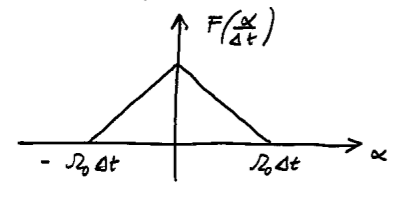
\includegraphics{figuras/12-0}
\end{figure}

Como $\Phi(\alpha)$ é uma combinação de $F(\alpha / \Delta t + k 2 \pi / \Delta
t)$ para diferentes valores de $k$ e o gráfico dessas funções são translações
por $k 2 \pi / \Delta t$ do gráfico de $F(\alpha / \Delta t)$, podemos ter uma
das situações abaixo:
\begin{figure}[htb]
  \centering
  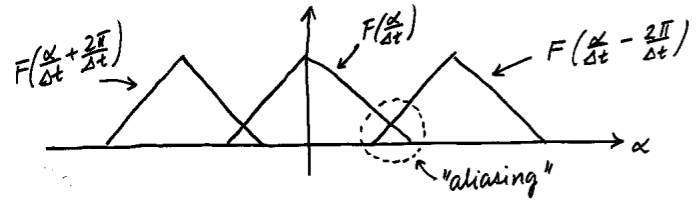
\includegraphics{figuras/12-1} \\
  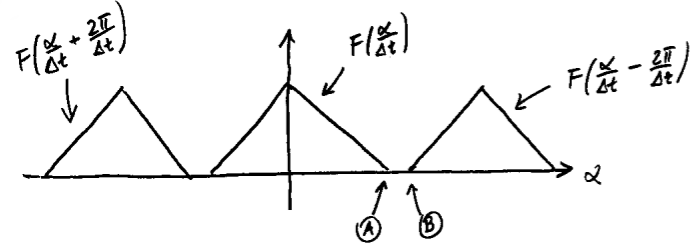
\includegraphics{figuras/12-2}
\end{figure}

É óbvio que apenas no segundo caso a soma dos perfis deslocados não altera o
perfil original. Note que nesse caso para os pontos $A$ e $B$ temos $x(B) - x(A)
\geq 0$. Se $F(x) = 0$ para $\lvert x \rvert \geq \Omega_0$, então $x(A) =
\Omega_o \Delta t$ e $x(B) = - \Omega_0 \Delta t + 2 \pi$, de modo que devemos
ter $-\Omega_0 \Delta t + 2 \pi - \Omega_0 \Delta t \geq 0$ e portanto
\begin{dmath*}
  \Omega_0 \Delta t \leq \pi.
\end{dmath*}
Além disso, camo $-\pi \leq \alpha \leq \pi$ e $x(\theta)$ nesse caso satisfaz
$x(\theta) \geq 2 \pi - \pi \geq \pi$, só temos a contribuição para
$\Phi(\alpha)$ da parte com $k = 0$, ou seja,
\begin{dmath*}
  \Phi(\alpha) = \frac{\sqrt{2 \pi}}{\Delta t} F\left( \frac{\alpha}{\Delta t} \right)
\end{dmath*}
se $F(x) = 0$, $\lvert x \rvert \geq \Omega_0$ e $\Omega_0 \Delta t \leq \pi$.
Nessas condições podemos reconstruir $f(t)$. De fato:
\begin{dmath*}
  f(t) = \frac{1}{\sqrt{2 \pi}} \int_{-\infty}^{+\infty} F(w) \exp(-i w t)
  \vi{w}
  = \frac{1}{\sqrt{2 \pi}} \int_{-\Omega_0}^{+\Omega_0} F(w) \exp(-i w t) \vi{w}
  = \frac{1}{\sqrt{2 \pi}} \int_{-\Omega_0 \Delta t}^{+\Omega \Delta t} F\left(
  \frac{\alpha}{\Delta t} \right) \exp(-i \alpha t / \Delta t)
  \frac{\vi{\alpha}}{\Delta t}
  = \frac{1}{2 \pi} \int_{-\Omega_0 \Delta t}^{+\Omega_0 \Delta t} \Phi(\alpha)
  \exp(-i \alpha t / \Delta t) \vi{\alpha}
  = \frac{1}{2 \pi} \int_{-\Omega_0 \Delta t}^{+\Omega_0 \Delta t} \left(
  \sum_{n = -\infty}^{+\infty} f_n \exp(i n \alpha) \right) \exp(-i \alpha t /
  \Delta t) \vi{\alpha}
  = \frac{1}{2 \pi} \sum_{n = -\infty}^{+\infty} f_n \left.
  \frac{\exp(i \alpha (n - t / \Delta t)}{i (n - t / \Delta t)}
  \right|_{-\Omega_0 \Delta t}^{+\Omega_0 \Delta t}
  = \frac{1}{\pi} \sum_{n = -\infty}^{+\infty} \frac{f_n}{(n - t / \Delta t)}
  \frac{\left[ \exp(i \Omega_0 \Delta t (n - t / \Delta t)) - \exp(-i \Omega_0
  \Delta t (n - t / \Delta t)) \right]}{2 i},
\end{dmath*}
ou seja,
\begin{dmath*}
  f(t) = \frac{\Delta t}{\pi} \sum_{n = -\infty}^{+\infty} f_n
  \frac{\sin(\Omega_0) (t - n \Delta t)}{t - n \Delta t}.
\end{dmath*}

Essa fórmula para reconstruir $f(t)$ á partir de $f_n$ é a essência do Teorema
da Amostragem de Shannon. Devemos lembrar as condições para que essa
reconstrução seja possível:
\begin{itemize}
  \item $F(w)$ deve ter suorte limitado ($F(w) = 0$ para $\lvert w \rvert \geq
    \Omega_0$), e
  \item o intervalo de amostragem deve satisfazer $\Delta t \leq \pi / \Omega_0$
    ou em termos da frequência de amostragem $\nu = 2 \pi / \Delta t$, $\nu \geq
    2 \Omega_0$.
\end{itemize}
A frequência $2 \Omega_0$ é chamada frequência de Nyquist. Podemos resumir nossa
situação através do diagrama:
\begin{figure}[htb]
  \centering
  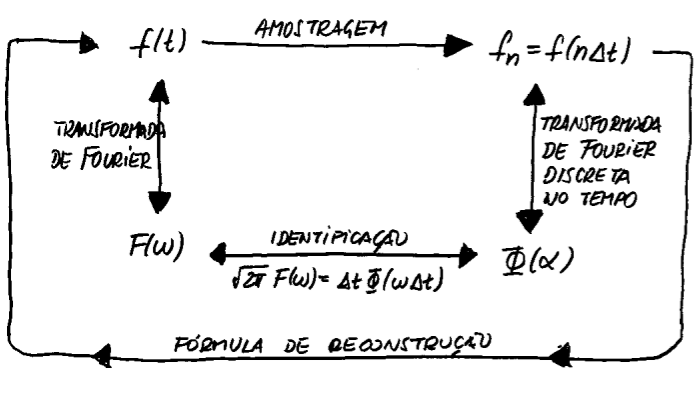
\includegraphics{figuras/12-3}
\end{figure}

\section{Transformada de Fourier Discreta}
Vamos agora estudar o caos em que temos apenas um número finito $f_0, f_1,
\ldots, f_{n - 1}$ de valores de $f(t)$ para o intervalo finito $[0, T]$, de
modo que dividindo o intervalo $[0, T]$ em $N$ pontos $t_k$,
\begin{dmath*}
  t_k = K T / N \condition{$k = 0, 1, \ldots, N - 1$,}
\end{dmath*}
temos $f_k = f(t_k)$.

Para isso vamos considerar a identidade
\begin{dmath*}
  q^N - 1 = (q - 1) (1 + q + q^2 + \ldots q^{N - 1}).
\end{dmath*}
Se $q^N = 1$ concluímos que $q^N - 1 = 0$ e portanto $q = 1$ ou $1 + q + \ldots
+ q^{N - 1} = 0$ se $q \neq 1$.

As raízes não triviais de $q^N = 1$ são da forma $\exp(n 2 \pi i / N)$, para $n
= 1, 2, \ldots, N - 1$, de modo que
\begin{dmath*}
  \sum_{k = 0}^{N - 1} q^k = \begin{cases}
    0, & \text{se } q = \exp(n 2 \pi i / N), n = 1, 2, 3, \ldots, N - 1, \\
    N, & \text{se } q = 1.
  \end{cases}
\end{dmath*}
Outra forma de escrevermos isso é fixando $q = \exp(2 \pi i / N)$ de modo que os
outros valores de $q$ são da forma $q^n$, $n = 0, 1, \ldots, N - 1$, e com isso
temos que
\begin{dmath*}
  \sum_{k = 0}^{N - 1} q^{n k} = N \delta_{n0},
\end{dmath*}
onde $\delta_{n0} = 0$ se $n \neq 0$ e $\delta_{n0} = 1$ se $n = 0$.

Definindo $w_n = n 2 \pi / T$ vemos que
\begin{dgroup*}
  \begin{dmath*}
    \exp(i w_n t_k) = \exp(i n (2 \pi / T) (k T / N))
    = \left( \exp(i 2 \pi / N) \right)^{n k}
    = q^{n k},
  \end{dmath*}
  \begin{dmath*}
    \left( \exp(i w_n t_k) \right)^k = \exp(-i w_n t_k)
    = q^{-n k}.
  \end{dmath*}
\end{dgroup*}
Com isso vemos que
\begin{dmath*}
  \sum_{k = 0}^{N - 1} \left( \exp(i w_n t_k) \right)^k \left( \exp(i w_m t_k)
  \right) = \sum_{k = 0}^{N - 1} q^{-n k} q^{m k}
  = \sum_{k = 0}^{N - 1} q^{(m - n) k},
  = N \delta_{mn}.
\end{dmath*}

Por outro lado,
\begin{dmath*}
  \sum_{n = 0}^{N - 1} \left( \exp(i w_n t_k \right)^k \exp(i w_n t_k) = \sum_{n
  = 0}^{N - 1} q^{-n k} q^{n l}
  = \sum_{n = 0}^{N - 1} q^{n (l - k)}
  = N \delta_{k l}.
\end{dmath*}

Isso nos sugere definir $F(w_n)$, $n = 0, 1, \ldots, N - 1$, como
\begin{dmath*}
  F(w_n) = \sum_{k = 0}^{N - 1} f(t_k) \exp(i w_n t_k).
\end{dmath*}
Com isso:
\begin{dmath*}
  \sum_{n = 0}^{N - 1} F(w_n) \left( \exp(i w_n t_l \right)^k = \sum_{n = 0}^{N
  - 1} \sum_{k = 0}^{N - 1} f(t_k) \exp(i w_n t_k) \exp(-i w_n t_l)
  = \sum_{k = 0}^{N - 1} f(t_k) \sum_{n = 0}^{N - 1} q^{n k} q^{-n l}
  = \sum_{k = 0}^{N - 1} f(t_k) N \delta_{kl}
  = N f(t_l),
\end{dmath*}
ou seja,
\begin{dmath*}
  f(t_k) = \frac{1}{N} \sum_{n = 0}^{N - 1} F(w_n) \exp(-i w_n t_k).
\end{dmath*}

Portanto $F(w_n)$ é a transformada de Fourier discreta e $f(t_k)$ a sua
transformada inversa.

Podemos notar que
\begin{dmath*}
  F(w_n) = \sum_{k = 0}^{N - 1} f(t_k) g^{n k}
\end{dmath*}
pode ser escrita numa forma matricial, ou seja,
\begin{dmath*}
  F = Q_N f,
\end{dmath*}
onde $Q_N$ é chamada matriz de Fourier,
\begin{dmath*}
  \begin{bmatrix}
    F(w_0) \\
    F(w_1) \\
    \vdots \\
    F(w_{N - 1})
    \end{bmatrix} = \begin{bmatrix}
    q^{00} & q^{01} & \ldots & q^{0(N - 1)} \\
    q^{10} & q^{11} & \ldots & q^{1(N - 1)} \\
    \vdots & \vdots & \ddots & \vdots \\
    q^{(N - 1)0} & q^{(N - 1)1} & \ldots & q^{(N - 1)(N - 1)}
  \end{bmatrix} \begin{bmatrix}
    f(t_0) \\
    f(t_1) \\
    \vdots \\
    f(t_{N - 1})
  \end{bmatrix}
\end{dmath*}

Como podemos ver, a matriz $Q_N$ apresenta uma grande redundância. De fato:
\begin{dmath*}
  Q_N =  \begin{bmatrix}
    1 & 1 & 1 & \ldots & 1 \\
    1 & q^{1} & q^{2} & \ldots & q^{(N - 1)} \\
    1 & q^{2} & q^{4} & \ldots & q^{2(N - 1)} \\
    \vdots & \vdots & \vdots & \ddots & \vdots \\
    1 & q^{(N - 1)} & q^{2 (N - 1)} & \ldots & q^{(N - 1)(N - 1)}
  \end{bmatrix}
\end{dmath*}

Podemos eliminar um pouco dessa redundância através de um algoritmo chamado
``transformada de Fourier rápida''\footnote{Em inglês, Fast Fourier Transform ou
FFT.}. Para isso é essencial que o número de pontos seja $2^n$, ou seja, $N =
2^n$. Vamos ainda denotar $N_k = 2^{n - k}$ de modo que $N = 2^K N_k$, $k = 0,
1, \ldots, n$.

Considerando $F(w_n)$, podemos escrever ($N = 2 N_1$)
\begin{dmath*}
  F(w_n) = \sum_{k = 0}^{N - 1} f(t_k) g^{n k}
  = \sum_{k = 0}^{N_1 - 1} f(t_k) g^{n k} + \sum_{k = N_1}^{2 N_1 - 1} f(t_k)
  q^{n k}
  = \sum_{k = 0}^{N_1 - 1} f(t_k) g^{n k} + \sum_{k = 0}^{N_1 - 1} f(t_{(k +
  N_1)}) q^{n (k + N_1)}.
\end{dmath*}
Mas
\begin{dmath*}
  q = \exp(2 \pi i / N)
  = \exp(2 \pi i / (2 N_1))
  = \exp(\pi i / N_1),
\end{dmath*}
ou seja, $q^{N_1} = \exp(\pi i) = -1$ e $q^{n N_1} = (-1)^n$. Logo:
\begin{dmath*}
  F(w_n) = \sum_{k = 0}^{N_1 - 1} f(t_k) q^{n k} + \sum_{k = 0}^{N_1 - 1} f(t_{k
  + N_1}) g^{n k} (-1)^n
  = \sum_{k = 0}^{N_1 - 1} \left[ f(t_k) + (-1)^n f(t_{k + N_1}) \right] g^{n
  k}.
\end{dmath*}
De modo que
\begin{dgroup*}
  \begin{dmath*}
    F(w_{2 n_1}) = \sum_{k = 0}^{N_1 - 1} \left[ f(t_k) + f(t_{k + N_1}) \right]
    \left( q^2 \right)^{k n_1},
  \end{dmath*}
  \begin{dmath*}
    F(w_{2 n_1 + 1}) = \sum_{k = 0}^{N_1 - 1} \left[ f(t_k) - f(t_{k + N_1})
    \right] \left( q^2 \right)^{K n_1} q^k,
  \end{dmath*}
\end{dgroup*}
para $n_1 = 0, 1, \ldots, N_1 - 1$.

Como a matriz $Q_N$ é $N \times N = 2^n 2^n = 2^{2n}$, agora temos $2 N_1 N_1 =
2 2^{n - 1} 2^{n - 1} = 2^{2 n - 1}$, ou seja, o número de operações
(multiplicações) é reduzido pela metade.

Uma forma de olhar para o procedimento acima é notando que
\begin{dmath*}
  q^2 = \left( \exp(2 \pi i / N) \right)^2
  = \exp(2 \pi i / (N / 2))
  = \exp(2 \pi i / N_1)
  = q_1,
\end{dmath*}
ou seja, $(q^2)^{k n_1}$, $k_1 n_1 = 0, 1, \ldots, N_1 - 1$, são entradas da
matriz de Fourier para $N_1$, ou seja,
\begin{dmath*}
  \begin{bmatrix}
    F(w_0) \\
    F(w_1) \\
    \vdots \\
    F(w_{2 N_1 - 1})
  \end{bmatrix} =  \begin{bmatrix}
    1 & 1 & \ldots & 1 \\
    1 & q^{2} & \ldots & q^{(N - 1)} \\
    1 & q^{4} & \ldots & q^{2(N - 1)} \\
    \vdots & \vdots & \ddots & \vdots \\
    1 & q^{2 (N - 1)} & \ldots & q^{(N - 1)(N - 1)}
  \end{bmatrix} \begin{bmatrix}
    f(t_0) + f(t_{N_1}) \\
    f(t_1) + f(t_{N_1 + 1})\\
    \vdots \\
    f(t_{N - 1}) + f(t_{2 N_1})
  \end{bmatrix}
\end{dmath*}

% TODO Terminar M2S12-12.pdf. Interrompido na página 15.

% Filename: cap05@notas_de_aula.tex
% This code is part of 'Notas de aula não oficiais de MS650 e F620'
% 
% Description: This file correspond to part of the textbook using in the course.
% 
% Created: 01.09.12 10:43:23 AM
% Last Change: 01.09.12 10:43:23 AM
% 
% Authors:
% - Raniere Silva, r.gaia.cs@gmail.com
% 
% Copyright (c) 2012, Raniere Silva. All rights reserved.
% 
% This work is licensed under the Creative Commons Attribution-NonCommercial-NoDerivs 3.0 Unported License. To view a copy of this license, visit http://creativecommons.org/licenses/by-nc-nd/3.0/.
%
% This work is distributed in the hope that it will be useful, but WITHOUT ANY WARRANTY; without even the implied warranty of MERCHANTABILITY or FITNESS FOR A PARTICULAR PURPOSE.
%
\chapter{Transformadas de Laplace}
\section{Definições e exemplos}
Vamos considerar uma série de potências
\begin{dmath*}
  f(x) = \sum_{k = 0}^{\infty} a_k x^k \condition{$|x| \leq h$.}
\end{dmath*}
Uma forma de generalizar essa série é considerando uma sequência ${\lambda_k}_{k
= 0}^{\infty}$ tal que
\begin{dgroup*}
  \begin{dmath*}
    0 \hiderel{\leq} \lambda_0 \hiderel{<} \lambda_1 \hiderel{<} \lambda_2
    \hiderel{<} \ldots,
  \end{dmath*}
  \begin{dmath*}
    \lim_{k \to \infty} \lambda_k = +\infty
  \end{dmath*}
\end{dgroup*}
e definindo
\begin{dmath*}
  f(x) = \sum_{k = 0}^{\infty} a_k x^{\lambda_k}.
\end{dmath*}

Ocorre, porém, que essa definição requer um cuidado para lidar com os valores
negativos de $x$ pois podemos ter que extrair raízes de $x$ para certos valores
de $\lambda_k$. Para contornar essa situação, vamos considerar $x \geq 0$. Para
garantir isso, vamos tomar $x = \exp(-s)$ e definir
\begin{dmath*}
  F(s) \hiderel{=} f(\exp(-s)) = \sum_{k = 0}^{\infty} a_k \exp(-s \lambda_k).
\end{dmath*}

Essa série é chamada série de Dirichlet. Uma vez que $\Delta k = (k + 1) - k =
1$, temos
\begin{dmath*}
  F(s) = \sum_{k = 0}^{\infty} a_k \exp(-s \lambda_k) \Delta k
\end{dmath*}
e asumindo que $k$ tome valores contínuos e depois o limite $\Delta k \to 0$
segue que
\begin{dmath*}
  F(x) = \int_0^{\infty} a(k) \exp(-s \lambda(k)) \vi{k}.
\end{dmath*}
A transformada de Laplace corresponde ao caso $\lambda(k) = k$.

\begin{defi}
  Dada a função $f(t)$, $0 \leq t \leq \infty$, definimos sua transformadas de
  Laplace como sendo a função $F(s)$ dada por
  \begin{dmath*}
    F(s) \hiderel{=} \mathcal{L}[f(t)] = \int_0^{\infty} f(t) \exp(-s t) \vi{t}
  \end{dmath*}
  definida para os valores de $s$ tais que a integral acima exista. Em geral $s
  \in \mathbb{C}$.
\end{defi}

\begin{exem}
  Vamos calcular a transformada de Laplace para $f(t) = 1$.
  \begin{dmath*}
    \mathcal{L}[1] = \int_0^{\infty} \exp(-s t) \vi{t}
    = \left. - \exp(-s t) / s \right|_0^{\infty}
    = 1 / s \condition{$s > 0$.}
  \end{dmath*}
\end{exem}

\begin{exem}
  Vamos calcular a transformada de Laplace para $f(t) = t^{\alpha}$.
  \begin{dmath*}
    \mathcal{L}[t^{\alpha}] = \int_0^{\infty} t^{\alpha} \exp(-s t) \vi{t}
    = \frac{1}{s^{\alpha + 1}} \int_0^{\infty} y^{\alpha} \exp(-y) \vi{y}
    = \frac{1}{s^{\alpha + 1}} \Gamma(\alpha + 1)
    = \frac{n!}{s^{\alpha + 1}} \condition{$s > 0$.}
  \end{dmath*}
\end{exem}

\begin{exem}
  Vamos calcular a transformada de Laplace para $f(t) = \sin(kt)$.

  Uma vez que
  \begin{dmath*}
    \int \sin(k t) \exp(-s t) \vi{t} = \frac{-1}{k^2 + s^2} \left[ s \exp(-s t)
    \sin(k t) + k \exp(-s t) \cos(k t) \right],
  \end{dmath*}
  temos
  \begin{dmath*}
    \mathcal{L}[\sin(k t)] = \left. \frac{-1}{k^2 + s^2} \left[ s \exp(-s t) + k
    \exp(-s t) \cos(k t) \right] \right|_0^{\infty}
    = \frac{-1}{k^2 + s^2} [-k]
    = \frac{k}{k^2 + s^2} \condition{$s > 0$.}
  \end{dmath*}
  Analogamente,
  \begin{dmath*}
    \mathcal{L}[\cos(k t)] = \frac{s}{k^2 + s^2} \condition{$s > 0$.}
  \end{dmath*}
\end{exem}

\begin{exem}
  Vamos calcular a transformada de Laplace para $f(x) = \exp(a t)$.
  \begin{dmath*}
    \mathcal{L}[\exp(a t)] = \int_0^{\infty} \exp(-s t) \exp(a t) \vi{t}
    = \int_0^{\infty} \exp(- (s - a) t) \vi{t}
    = \left. \frac{\exp(- (s - a) t)}{- (s - a)} \right|_0^{\infty}
    = 1 / (s - a) \condition{$s - a > 0$.}
  \end{dmath*}
\end{exem}

\begin{defi}
  Uma função $f(t)$ definida no intervamo $a \leq t < \infty$ é de ordem
  exponencial $\sigma_0$ ($\sigma_0 \in \mathbb{R}$) se
  \begin{dmath*}
    | \exp(-\sigma_0 t) f(t) | \leq M,
  \end{dmath*}
  onde $M$ é uma constante positiva.
\end{defi}

\begin{teo}
  Se $f(t)$ pe contínua por partes para $0 \leq t < \infty$ e é exponencial de
  ordem $\sigma_0$, então a integral de Laplace
  \begin{dmath*}
    F(s) \hiderel{=} \mathcal{L}[f(t)] = \int_0^{\infty} \exp(-s t) f(t) \vi{t}
  \end{dmath*}
  converge para $\Re(s) > \sigma_0$. Além disso, a integral é absoluta e
  uniformemente convergente para $\Re(s) \geq \sigma_1$ se $\sigma_1 >
  \sigma_0$.
\end{teo}
\begin{proof}
  Para $s = \sigma + i w$, temos que
  \begin{dmath*}
    F_R(s) = \int_0^R \exp(-s t) f(t) \vi{t}.
  \end{dmath*}
  % TODO Terminar a demonstração. M2S12-13.pdf página 5.
\end{proof}

\section{Propriedades}
Antes de começarmos a listar algumas propriedades das transformada de Laplace,
devemos notar que duas funções $f_1(t)$ e $f_2(t)$ tais que
\begin{dgroup*}
  \begin{dmath*}
    f_1(t) = f_2(t) \condition{$0 \leq t < \infty$}
  \end{dmath*}
  \begin{dmath*}
    f_1(t) \neq f_2(t) \condition{$t < 0$}
  \end{dmath*}
\end{dgroup*}
tem a mesma transformada de Laplace. Para evitar essa ambiguidade, vamos
estabelecer que sempre que falamos em uma função $f(t)$ estamos nos referindo à
função $f_N(t)$,
\begin{dmath*}
  f_H(t) \hiderel{=} f(t) H(t) = \begin{cases}
    f(t), & t \geq 0, \\
    0, & t < 0,
  \end{cases}
\end{dmath*}
onde $H(t)$ é a função escada de Heaviside.

\begin{lem}[Translação]
  Se $\mathcal{L}[f(t)] = F(s)$, então para $a < 0$:
  \begin{dgroup*}
    \begin{dmath*}
      \mathcal{L}[f_H(t - a)] = \exp(-a s) F(s),
    \end{dmath*}
    \begin{dmath*}
      \mathcal{L}[\exp(- a t) f(t)] = F(s + a).
    \end{dmath*}
  \end{dgroup*}
\end{lem}
\begin{proof}
  Temos que
  \begin{dmath*}
    \mathcal{L}[f_H(t - a)] = \int_0^{\infty} \exp(-s t) f_H(t - a) \vi{t}
    = \int_0^{\infty} \exp(-s t) f(t - a) H(t - a) \vi{t}
    = \int_a^{\infty} \exp(-s t) f(t - a) \vi{t}
    = \int_0^{\infty} \exp(-s (u + a)t) f(u) \vi{u}
    = \exp(-a s) \mathcal{L}[f(t)].
  \end{dmath*}

  Podemos notar que essa propriedade não vale para $a < 0$ pois nesse caso
  teríamos, se $a < 0$
  \begin{dmath*}
    \int_0^{\infty} \exp(-s t) f_H(t - a) \vi{t} = \int_0^{\infty} \exp(-s t)
    f(t - a) \vi{t}
  \end{dmath*}
  que não guarda a relação acima com $\mathcal{L}[f(t)]$.

  Quanto á outra relação:
  \begin{dmath*}
    \mathcal{L}[\exp(-a t) f(t)] = \int_0^{\infty} \exp(-s t) \exp(-a t) f(t)
    \vi{t}
    = \int_0^{\infty} \exp(-(s + a) t) f(t) \vi{t}
  \end{dmath*}
  e se $\mathcal{L}[f(t)] = F(s)$ existe para $s > \sigma_0$, então para existir
  $\mathcal{L}[\exp(-a t) f(t)]$ devemos ter $s + a > \sigma_0$, ou seja, $a >
  0$.
\end{proof}

\begin{lem}[Derivação]
  As seguintes relações são válidas:
  \begin{dgroup*}
    \begin{dmath*}
      \mathcal{L}[f'(t)] = s \mathcal{L}[f(t)] - f(0),
    \end{dmath*}
    \begin{dmath*}
      F'(s) = - \mathcal{L}[t f(t)].
    \end{dmath*}
  \end{dgroup*}
\end{lem}
\begin{proof}
  Temos que
  \begin{dmath*}
    \int_0^{\infty} \exp(-s t) f'(t) \vi{t} = \left. \exp(-s t) f(t)
    \right|_0^{\infty} + s \int_0^{\infty} \exp(-s t) f(t) \vi{t}
    = - f(0) + s \mathcal{L}[f(t)],
  \end{dmath*}
  onde claramente devemos interpretar $f(0$ como $f(0^+)$.

  Já a outra propriedade:
  \begin{dmath*}
    F'(s) = \fder{}{s} \int_0^{\infty} \exp(-s t) f(t) \vi{t}
    = \int_0^{\infty} \exp(-s t) (-k) f(t) \vi{t}
    = - \mathcal{L}[t f(t)].
  \end{dmath*}
\end{proof}

Para generalizar essas expressões notamos que
\begin{dmath*}
  L[f''(t)] = \mathcal{L}[(f'(t))']
  = s \mathcal{L}[f'(t)] - f'(0)
  = s [s \mathcal{L}[f(t) - f(0)] - f'(0),
\end{dmath*}
ou seja,
\begin{dmath*}
  \mathcal{F}[f''(t)] = s^2 \mathcal{L}[f(t)] - s f(0) - f'(0).
\end{dmath*}

As generalizações são, portanto:
\begin{dgroup*}
  \begin{dmath*}
    \mathcal{L}[f^{(n)}(t)] = s^n \mathcal{L}[f(t)] - \sum_{k = 1}^n s^{k - 1}
    f^{(n - k)}(0),
  \end{dmath*}
  \begin{dmath*}
    F^{(n)}(s) = (-1)^n \mathcal{L}[t^n f(t)].
  \end{dmath*}
\end{dgroup*}

\section{Convolução}
Quando estudamos as transformada de Fourier nós definimos a convolução $(f +
g)(t)$ como
\begin{dmath*}
  (f + g)(t) = \frac{1}{\sqrt{2 \pi}} \int_{-\infty}^{+\infty} f(\tau) g(t -
  \tau) \vi{\tau}.
\end{dmath*}

A presença do fator $\sqrt{2 \pi}$ se fez necessária para podermos escrever o
teorema da convolução na forma $\mathcal{F}[f * g] = \mathcal{F}[f]
\mathcal{F}[g]$ visto que na definição de $\mathcal{F}$ havia um fator $\sqrt{2
\pi}$. Ocorre que na transformada de Laplace não existe esse fator, de modo que
pensando dentro do contexto da teoria das transformada de Laplace é melhor
redefinir a convolução sem o fator $\sqrt{2 \pi}$. Sendo assim, tomamos
\begin{dmath*}
  (f_H * g_H)(t) = \int_{-\infty}^{+\infty} f_H(\tau) g_H(t - \tau) \vi{\tau}
  = \int_0^{\infty} f(\tau) g_H(t - \tau) \vi{\tau}
\end{dmath*}
e como $g_H(t - \tau) = 0$ para $t - \tau < 0$, ou seja, para $\tau > t$, temos
\begin{dmath*}
  (f_H * g_H)(t) = \int_0^t f(t) g(t - \tau) \vi{\tau}.
\end{dmath*}
Iremos escrever simplesmente $(f * g)(t)$ lembrando que estamos dentro do
contexto das transformadas de Laplace.

Antes de nos perguntarmos pela transformada de Laplace da convolução, vamos ver
se ela é de ordem exponencial quando $f$ e $g$ forem, o que irá garantir a
existência da transformada em um certo intervalo. Se $|f(t)| \leq M_1
\exp(\alpha t)$ e $|g(t)| \leq M_2 \exp(\beta t)$, então
\begin{dmath*}
  \lvert f * g \rvert \leq \int_0^{t} \lvert f(\tau) \rvert \lvert g(t - \tau)
  \rvert \vi{\tau}
  \leq M_1 M_2 \int_0^{t} \exp(\alpha \tau) \exp(\beta (t - \tau)) \vi{\tau}
  \leq M_1 M_2 \exp(\beta t) \int_0^t \exp( (\alpha - \beta) ) \vi{\tau}
  \leq M_1 M_2 \exp(\beta t) \int_0^t \exp( (\alpha - \beta) \tau) \vi{\tau}.
\end{dmath*}
\begin{enumerate}
  \item se $\alpha = \beta$:
    \begin{dmath*}
      \lvert f * g \rvert \leq M_1 M_2 \exp(\beta t) \int_0^t \vi{\tau}
      = M_1 M_2 \exp(\beta t) t
    \end{dmath*}
    e como $\exists M_3 > 0, \epsilon > 0$ tal que $t < M_3 \exp(\epsilon t)$,
    temos
    \begin{dmath*}
      \lvert f * g \rvert \leq M_1 M_2 M_3 \exp( (\beta + \epsilon) t)
    \end{dmath*}

  \item se $\alpha \neq \beta$:
    \begin{dmath*}
      \lvert f * g \rvert \leq M_1 M_2 \exp(\beta t) \left. \frac{\exp( (\alpha - \beta)
      \tau)}{\alpha - \beta} \right|_0^t
      = M_1 M_2 \left( \frac{\exp(\alpha t) - \exp(\beta t)}{\alpha - \beta}
      \right).
    \end{dmath*}
    Quando $\alpha > \beta$:
    \begin{dmath}
      \frac{\exp(\alpha t) - \exp(\beta t)}{\alpha - \beta} <
      \frac{\exp(\alpha t)}{\alpha - \beta}.
    \end{dmath}
    E quando $\beta < \alpha$:
    \begin{dmath*}
      \frac{\exp(\alpha t) - \exp(\beta t)}{\alpha - \beta} =
      \frac{\exp(\beta t) - \exp(\alpha t)}{\beta - \alpha}
      < \frac{\exp(\beta t)}{\beta - \alpha}.
    \end{dmath*}
    Portanto:
    \begin{dmath*}
      \lvert f * g \rvert \leq M \exp(\gamma t),
    \end{dmath*}
    para $\gamma = \max(\alpha, \beta) + \epsilon > \max(\alpha, \beta)$.
\end{enumerate}

\begin{teo}[Convolução]
  Se $f(t)$ e $g(t)$ são contínuas por partes e de ordens exponenciais $\alpha$
  e $\beta$, respectivamente, então
  \begin{dmath*}
    \mathcal{L}[(f * g)(t)] = \mathcal{L}[f(t)] \mathcal{L}[g(t)],
  \end{dmath*}
  para $\Re(s) > \max(\alpha, \beta)$.
\end{teo}
\begin{proof}
  Temos que
  \begin{dmath*}
    \mathcal{L}[(f * g)(t)] = \int_0^{\infty} \exp(-s t) (f * g)(t) \vi{t}
    = \int_{-\infty}^{+\infty} H(t) \exp(-s t) (f * g)(t) \vi{t}
    = \int_{-\infty}^{+\infty} H(t) \exp(-s t) \int_{-\infty}^{+\infty}
    f_H(\tau) g_H(t - \tau) \vi{\tau} \vi{t}
    = \int_{-\infty}^{+\infty} \int_{-\infty}^{+\infty} H(t) \exp(-s t) f(\tau)
    H(\tau) g(t - \tau) H(t - \tau) \vi{\tau} \vi{\tau}
    = \int_{-\infty}^{+\infty} \int_{-\infty}^{+\infty} H(u + \tau) \exp(-s (u +
    \tau)) f(\tau) H(\tau) g(u) H(u) \vi{\tau} \vi{u}
    = \int_0^{\infty} \int_0^{\infty} \exp(-s u) \exp(-s \tau) f(\tau) g(u) H(u
    + \tau) \vi{\tau} \vi{u}
    = \int_0^{\infty} \int_0^{\infty} \exp(-s u) \exp(-s \tau) f(\tau) g(u) 1
    \vi{\tau} \vi{u}
    = \int_0^{\infty} \int_0^{\infty} \exp(-s u) \exp(-s \tau) f(\tau) g(u)
    \vi{\tau} \vi{u}
    = \int_0^{\infty} \exp(-s u) g(u) \int_0^{\infty} \exp(-s \tau) f(\tau)
    \vi{\tau} \vi{u}
    = \mathcal{L}[f(t)] \mathcal{L}[g(t)].
  \end{dmath*}
\end{proof}

\section{A Tranformação Inversa}
Para chegarmos a uma expressão para a transformação inversão, vamos explorar a
relação entre as transformadas de Fourier e Laplace. Dada $f_H(t) = f(t) H(t)$,
temos
% TODO Revisão a equação abaixo. M2S12-14.pdf página 1.
\begin{dmath*}
  \int_{-\infty}^{+\infty} f_H(t) \exp(-s t) \exp(i k t) \vi{t} =
  \mathcal{L}[f_H(t) \exp(i k t)](s)
  = \sqrt{2 \pi} \mathcal{F}[f_H(t) \exp(-s t)](k)
\end{dmath*}

Temos
\begin{dmath*}
  f_H(t) \exp(-s t) = \mathcal{F}^{-1}[F_S(k)](t)
  = \frac{1}{\sqrt{2 \pi}} \int_{-\infty}^{+\infty} F_S(k) \exp(-i k t) \vi{k}
  = \frac{1}{\sqrt{2 \pi}} \int_{+i \infty + s}^{-i \infty + s} F_S(i z + i
  \beta) \exp(-i (i z - i s) t) \frac{\vi{z}}{-i}
  = \frac{1}{\sqrt{2 \pi}} \int_{+i \infty + s}^{-i \infty + s}
  \mathcal{F}[f_H(t)](i z - i s + i s) \exp(-i (i z - i s) t)
  \frac{\vi{z}}{-i}
  = \frac{1}{\sqrt{2 \pi} i} \int_{-i \infty + s}^{+i \infty + s}
  \mathcal{F}[f_H(t)](i z) \exp(z t) \exp(-s t) \vi{z}
  = \frac{1}{\sqrt{2 \pi} i} \int_{-i \infty + s}^{+i \infty + s}
  \frac{1}{\sqrt{2 \pi}} \mathcal{L}[f_H(t)](z) \exp(z t) \exp(-s t) \vi{z}
  = \exp(-s t) \frac{1}{2 \pi i} \int_{-i \infty + s}^{+i \infty + s}
  \mathcal{L}[f_H(t)](z) \exp(z t) \vi{z}
\end{dmath*}
o que nos sugere que, para $F(s) = \int_0^{\infty} \exp(-s t) f(t) \vi{t}$, temos
\begin{dmath*}
  f_H(t) = \frac{1}{2 \pi i} \int_{-i \infty + \gamma}^{+i \infty + \gamma}
  \exp(s t) F(s) \vi{s}
\end{dmath*}
para $\gamma$ convenientemente escolhido. Vamos verificar que essa fórmula de
fato vale, com $\gamma$ escolhido de modo que todas as possíveis singularidades
de $\exp(s t) F(s)$ fiquem à esquerda de $\gamma$, ou seja,
\begin{figure}[htb]
  \centering
  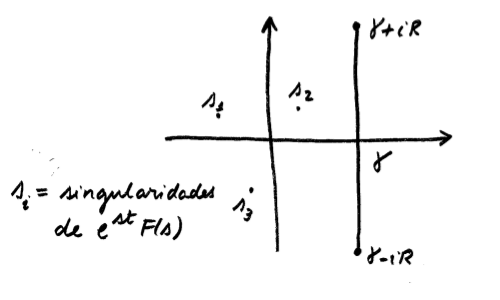
\includegraphics{figuras/14-0}
\end{figure}

Vamos calcular $I_R(t)$:
\begin{dmath*}
  I_R(t) = \frac{1}{2 \pi i} \int_{\gamma - i R}^{\gamma + i R} \exp(s t) F(s)
  \vi{s}
  = \frac{1}{2 \pi i} \int_{\gamma - i R}^{\gamma + i R} \exp(s t)
  \int_0^{\infty} \exp(-s z) f(z) \vi{z} \vi{s}
  = \frac{1}{2 \pi i} \int_0^{\infty} f(z) \int_{\gamma - i R}^{\gamma + i R}
  \exp(s (t - z)) \vi{s} \vi{z}
  = \frac{1}{2 \pi i} \int_0^{\infty} f(z) \left. \frac{\exp(s (t - z))}{t - z}
  \right|_{\gamma - i R}^{\gamma + i R} \vi{z}
  = \frac{1}{2 \pi i} \int_0^{\infty} f(z) \exp(\gamma (t - z))
  \frac{\exp(i R (t - z)) - \exp(-i R (t - z))}{t - z} \vi{z}
  = \frac{1}{\pi} \int_0^{\infty} f(z) \exp(\gamma (t - z))
  \frac{\sin(R (t - z))}{t - z} \vi{z}
  = \frac{1}{\pi} \int_{-t}^{\infty} f(t + u) \exp{-\gamma u}
  \frac{\sin(R u)}{u} \vi{u}
  = \frac{1}{\pi} \int_{-t}^0 f(t + u) \exp(-\gamma u) \frac{\sin(R u)}{u}
  \vi{u} + \frac{1}{\pi} \int_0^{\infty} f(t + u) \exp(-\gamma u)
  \frac{\sin(R u)}{u} \vi{u}
\end{dmath*}
% TODO Informar número da página.
Mas do lema das páginas ?? e ?? sabemos que
\begin{dmath*}
  \lim_{k \to \infty} \int_0^b F(u) \frac{\sin(R u)}{u} F(u) = \lim_{k \to
  \infty} \int_0^{\infty} F(u) \frac{\sin(R u)}{u} \vi{u}
  = \frac{\pi}{2} F(0^+).
\end{dmath*}
Com isso, para $R \to \infty$, temos
\begin{dgroup*}
  \begin{dmath*}
    \lim_{R \to \infty} \frac{1}{pi} \int_0^{\infty} f(t + u) \exp(-\gamma u)
    \frac{\sin(R u)}{u} \vi{u} = \frac{1}{\pi} \frac{\pi}{2} f(t + 0)
    = \frac{1}{2} f(t^+),
  \end{dmath*}
  \begin{dmath*}
    \lim_{R \to \infty} \frac{1}{\pi} \int_{-t}^0 f(t + u) \exp(-\gamma u)
    \frac{\sin(R u)}{u} \vi{u} = \begin{cases}
      0, & t = 0, \\
      (1 / 2) f(t^-), & t > 0, \\
      (-1 / 2) f(t^+), & t < 0,
    \end{cases}
  \end{dmath*}
\end{dgroup*}
de modo que
\begin{dmath*}
  \lim_{R \to \infty} I_R(t) = \begin{cases}
    (1 / 2) f(0), & t = 0, \\
    (1 / 2) [f(t^+) + f(t^0)], & t > 0, \\
    0, & t < 0.
  \end{cases}
\end{dmath*}
De fato:
\begin{dmath*}
  f(t) H(t) = \frac{1}{2 \pi i} \int_{\gamma - i \infty}^{\gamma + i \infty}
  \exp(s t) F(s) \vi{s}
\end{dmath*}
que é chamada de integral de Bromwich ou integral de Mellin ou ainda integral de
Fourier-Mellin.

\begin{exem}
  Considere
  \begin{dmath*}
    F(s) = \frac{k}{s^2 - k^2}
    = \frac{k}{(s - k) (s + k)}.
  \end{dmath*}
  Então
  \begin{dmath*}
    f(t) = \frac{1}{2 \pi i} \int_{\gamma - i \infty}^{\gamma + i \infty} \exp(s
    t) \frac{k}{s^2 - k^2} \vi{s}
    = \left[ \Res_{s = k} + \Res_{s = -k} \right] \left( \frac{\exp(s t) k}{s^2
    - k^2} \right)
    = \frac{\exp(k t) k}{2 k} + \frac{\exp(-k t) k}{(-2 k)}
    = \frac{\exp(k t) - \exp(-k t)}{2}
    = \sinh(k t).
  \end{dmath*}
  \begin{figure}[htb]
    \centering
    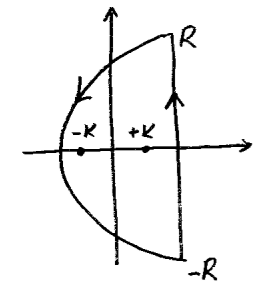
\includegraphics{figuras/14-1}
  \end{figure}
\end{exem}

\begin{exem}
  Considere $F(s) = 1 / \sqrt{s}$. Como $s = 0$ é um ponto de ramificação,
  \begin{figure}[htb]
    \centering
    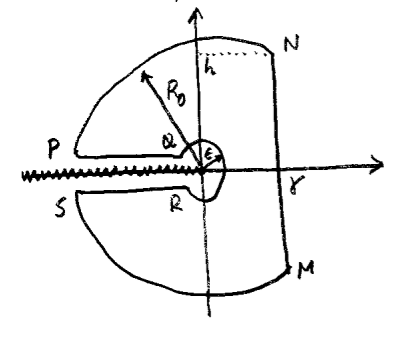
\includegraphics{figuras/14-2}
  \end{figure}
  temos
  \begin{dmath*}
    \int_M^N + \int_N^P + \int_P^Q + \int_Q^R + \int_R^S + \int_S^M = 0
  \end{dmath*}
  % TODO Terminar de digitar o exemplo. M2S12-14.pdf página 5.
\end{exem}

\begin{exem}
  Considere $F(s) = A(s) / B(s)$, com
  \begin{dmath*}
    B(s) = (s - s_1) \ldots (s - s_n) \condition{$s_1 \neq \ldots s_n$.}
  \end{dmath*}
  \begin{figure}[htb]
    \centering
    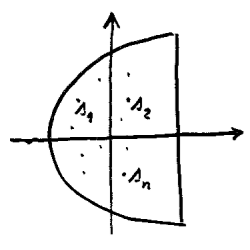
\includegraphics{figuras/14-3}
  \end{figure}
  Então,
  \begin{dmath*}
    f(t) = \frac{1}{2 \pi i} \int_{\gamma - i \infty}^{\gamma + i \infty}
    \frac{H(s) \exp(s t)}{(s - s_1) \ldots (s - s_n)} \vi{s}
    = \sum_{i = 1}^n \Res_{s = s_i} \left[ \frac{A(s) \exp(s t)}{(s - s_1)
    \ldots (s - s_n)} \right]
    = \sum_{i = 1}^n \lim_{s \to s_1} \left[ \frac{(s - s_i) A(s) \exp(s t)}{(s
    - s_1) \ldots (s - s_n)} \right]
    = \sum_{i = 1}^n \left[ \frac{A(s_i) \exp(s_i t)}{(s_i - s_1) \ldots (s_i -
    s_{i - 1}) (s_i - s_{i + 1} \ldots (s_i - s_n)} \right]
  \end{dmath*}
  Mas
  \begin{dmath*}
    B'(s) = (s - s_2) (s - s_3) \ldots (s - s_n) + (s - s_1) (s - s_3) \ldots (s
    - s_n) + \ldots + (s - s_1) (s - s_2) \ldots (s - s_{n - 1}),
  \end{dmath*}
  portanto,
  \begin{dmath*}
    B'(s_i) = (s_i - s_1) (s_i - s_2) \ldots (s_i - s_{i - 1})) (s_i - s_{i +
    1}) \ldots (s_i - s_n).
  \end{dmath*}
  Logo,
  \begin{dmath*}
    f(t) = \sum_{i = 1}^n \frac{A(s_i) \exp(s_i t)}{B'(s_i)}
  \end{dmath*}
\end{exem}

\begin{exem}
  Considere $F(s) = A(s) / (s - a)^n$.
  \begin{figure}[htb]
    \centering
    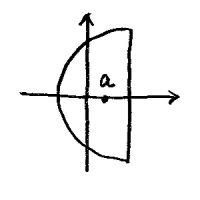
\includegraphics{figuras/14-4}
  \end{figure}
  Então,
  \begin{dmath*}
    f(t) = \frac{1}{2 \pi i} \int_{\gamma - i \infty}^{\gamma + i \infty}
    \frac{A(s) \exp(s t)}{(s - a)^n} \vi{s}
    = \Res_{s = 1} \left[ \frac{A(s) \exp(s t)}{(s - a)^n} \right]
    = \lim_{s \to a} \frac{1}{(n - 1)!} \fder{^{n - 1}}{s^{n - 1}} \left[ A(s)
    \exp(s t) \right]
    = \lim_{s \to a} \frac{1}{(n - 1)!} \sum_{k = 0}^{n - 1} \binom{n - 1}{k}
    A^{(k)}(s) t^{n - 1 - k} \exp(s t)
    = \sum_{k = 0}^{n - 1} \frac{1}{(n - 1 - k)! k!} A^{(k)}(a) t^{n - 1 - k}
    \exp(a t).
  \end{dmath*}

  Para $F(s) = A(s) / [(s - a_1)^{n_1} \ldots (s - a_i)^{n_i}]$ usamos a
  decomposição em frações parciais e aí a expressão acima para cada termo.
\end{exem}

\section{Algumas aplicações}
\begin{exem}[EDO de segunda ordem]
  Considere o sistema
  \begin{dmath*}
    \begin{cases}
      x'' + 2 \lambda x' + w_0^2 x = f(x), & w_o > \lambda, \\
      x(0) = x_0, \\
      x'(0) = v_0.
    \end{cases}
  \end{dmath*}
  Então,
  \begin{dgroup*}
    \begin{dmath*}
      \mathcal{L}[x'] = s \mathcal{L}[x] - x(0)
      = s X(s) - x_0,
    \end{dmath*}
    \begin{dmath*}
      \mathcal{L}[x''] = s^2 \mathcal{L}[x] - s x(0) - x'(0)
      = s^2 X(s) - s x_0 - v_0.
    \end{dmath*}
  \end{dgroup*}
  Portanto,
  \begin{dgroup*}
    \begin{dmath*}
      F(s) = s^2 X(s) - s x_0 - v_0 + 2 \lambda s X(s) - 2 \lambda x_0 + w_0^2
      X(s),
    \end{dmath*}
    \begin{dmath*}
      F(s) = \left( s^2 + 2 \lambda s + w_0^2 \right) X(s) - \left( 2 \lambda +
      s \right) x_0 - v_0,
    \end{dmath*}
    \begin{dmath*}
      X(s) = \frac{(2 \lambda + s) x_0 + v_0}{s^2 + 2 \lambda s + w_0^2} +
      \frac{F(s)}{s^2 + 2 \lambda s + w_0^2}.
    \end{dmath*}
    Mas:
    \begin{dmath*}
      s^2 + 2 \lambda s + w_0^2 = 0
    \end{dmath*}
    cuja solução é
    \begin{dmath*}
      s = - \lambda \pm i \sqrt{w_0^2 - \lambda^2} \condition{$w_0 > \lambda$.}
    \end{dmath*}
    % TODO Completar exemplo. M2S12-14.pdf pyágina 10.
  \end{dgroup*}
\end{exem}

\begin{exem}[EDP: Equação de Difusão]
  Considere o sistema
  \begin{dmath*}
    \begin{cases}
      \pder{u}{t} = \frac{1}{k^2} \pder{^2 u}{x^2}, & t \geq 0, x \geq 0, \\
      u(x, 0) = T_0, \\
      u(0, t) = T_1, \\
      \lim_{x \to \infty} u(x, t) < +\infty.
    \end{cases}
    % TODO Completar exemplo. M2S12-14.pdf pyágina 13.
  \end{dmath*}
\end{exem}

\begin{exem}
  A transformada de Laplace é particularmente útil para estudarmos expansões
  assintóticas. Dizemos que $\sum_{k = 0}^{\infty} a_k / z^k$ é uma expansão
  assintótica de $f(x)$ se
  \begin{dmath*}
    \lim_{\lvert z \rvert \to \infty} z^n \left[ f(z) - \sum_{k = 0}^n \frac{a_k}{z^k}
    \right] = 0 \condition{$n = 0, 1, 2, \ldots$,}
  \end{dmath*}
  e escrevemos
  \begin{dmath*}
    f(z) \sim \sum_{k = 0}^{\infty} \frac{a_k}{z^k}.
  \end{dmath*}

  Vamos supor que $f(t)$ tem a seguinte expansão em série de Taylor:
  \begin{dmath*}
    f(t) = \sum_{n = 0}^{\infty} a_n t^{\lambda_n - 1},
  \end{dmath*}
  onde $0 < \lambda_0 < \lambda_1 < \ldots$, e que seja de ordem exponencial
  para $t > a$,
  \begin{dmath*}
    \lvert f(t) \rvert < c \exp(b t).
  \end{dmath*}
  Seja agora
  \begin{dmath*}
    f_n(t) = f(t) - \sum_{k = 0}^n a_k t^{\lambda_k - 1}.
  \end{dmath*}
  Em função desses comportamentos para $t \to 0$ e $t > a$, existem constantes
  tais que
  \begin{dmath*}
    \lvert f_n(t) \rvert \leq c_n \exp(b t) t^{\lambda_{n + 1} - 1}.
  \end{dmath*}
  Por outro lado,
  \begin{dmath*}
    \mathcal{L}[f_n(t)] = \mathcal{L}[f(t)] - \sum_{k = 0}^n a_k L[t^{\lambda_k
    - 1}]
    = \mathcal{L}[f(t)] - \sum_{k = 0}^n a_k
    \frac{\Gamma(\lambda_k)}{s^{\lambda_k}}
  \end{dmath*}
  de modo que, se
  \begin{dmath*}
    \lim_{\lvert s \rvert \to \infty} \lvert s \rvert^{\lambda_n} \lvert
    \mathcal{L}[f_n(t)] \rvert = 0
  \end{dmath*}
  então temos
  \begin{dmath*}
    F(s) = \mathcal{F}[f(t)]
    \sim \sum_{k = 0}^{\infty} a_k \frac{\Gamma(\lambda_k)}{s^{\lambda_k}}.
  \end{dmath*}
  De fato:
  \begin{dmath*}
    \lvert\mathcal{L}[f_n(t)]\rvert \leq \int_0^{\infty} \lvert\exp(-s
    t)\rvert \lvert f_n(t) \rvert \vi{t}
    \leq \int_0^{\infty} \exp(-\Re(s) t) c_n \exp(b t) t^{\lambda_{n + 1} - 1}
    \vi{t}
    \leq c_n \int_0^{\infty} \exp(-\lvert s \rvert \cos(\varphi t) \exp(b t) t^{\lambda_{n
    + 1} - 1} \vi{t}
    = c_n \frac{\Gamma(\lambda_{n + 1}}{(\lvert s \rvert \cos(\varphi) - b)^{\lambda_{n +
    1}}},
  \end{dmath*}
  onde devemos ter $\lvert s \rvert \cos(\varphi) - b > 0$, o que
  necessariamente implica que $\cos(\varphi) > 0$, ou seja, $\arg(s) < \pi / 2$.

  Com isso,
  \begin{dmath*}
    \lim_{\lvert s \rvert \to \infty} \lvert s \rvert^{\lambda_{n}} \lvert
    \mathcal{L}[f_n(t)] \rvert \leq \lim_{\lvert s \rvert \to \infty}
    \frac{\lvert s \rvert^{\lambda_n} c_n \Gamma(\lambda_{n + 1})}{(\lvert s
    \rvert \cos(\varphi) - b)^{\lambda_{n + 1}}}
    = 0.
  \end{dmath*}
  Portanto, provamos o chamado Lema de Watson, ou seja, se $f(t) = \sum_{n =
  0}^{\infty} a_n t^{\lambda_{n - 1}}$ e é de ordem exponencial, então a sua
  transformada de Laplace $F(s)$ tem, para $\arg(s) < \pi / 2$, a segute
  expressão assintótica:
  \begin{dmath*}
    F(s) = \mathcal{L}[f(t)] \sim \sum_{k = 0}^{\infty} a_k
    \frac{\Gamma(\lambda_k)}{s^{\lambda_k}}.
  \end{dmath*}
  Por exemplo, para $f(t) = \ln(1 + \sqrt(t))$, temos
  \begin{dmath*}
    \ln(1 + \sqrt(t)) = \sum_{n = 1}^{\infty} \frac{(-1)^{n + 1} (\sqrt{t})^n}{n}
  \end{dmath*}
  e daí
  \begin{dmath*}
    \mathcal{L}[\ln(1 + \sqrt{t})] \sim \sum_{n = 1}^{\infty}
    \frac{(-1)^{n + 1}}{n} \frac{\Gamma(n / 2 + 1)}{s^{n / 2 + 1}}.
  \end{dmath*}
\end{exem}

% Filename: cap06@notas_de_aula.tex
% This code is part of 'Notas de aula n\~{a}o oficiais de MS650 e F620'
% 
% Description: This file correspond to part of the textbook using in the course.
% 
% Created: 01.09.12 10:43:23 AM
% Last Change: 01.09.12 10:43:23 AM
% 
% Authors:
% - Raniere Silva, r.gaia.cs@gmail.com
% 
% Copyright (c) 2012, Raniere Silva. All rights reserved.
% 
% This work is licensed under the Creative Commons Attribution-NonCommercial-NoDerivs 3.0 Unported License. To view a copy of this license, visit http://creativecommons.org/licenses/by-nc-nd/3.0/.
%
% This work is distributed in the hope that it will be useful, but WITHOUT ANY WARRANTY; without even the implied warranty of MERCHANTABILITY or FITNESS FOR A PARTICULAR PURPOSE.
%
\chapter{Transformadas Integrais: Outros Exemplos e Aplicações}
Uma transformada integral é uma transformação que leva uma função $f(x)$ em uma
função $F(y)$ através de
\begin{dmath*}
  F(y) = \int_{\alpha}^{\beta} K(x, y) f(x) \vi{x}
\end{dmath*}
Chamamos $K(x, y)$ de núcleo da transformada. Podemos ainda, no caso de
considerarmos variáveis complexas, tomar a integral acima ao londo de um caminho
no plano complexo. Os exemplos que já vimos são:
\begin{enumerate}
  \item Fourier: $\alpha = -\infty$, $\beta = +\infty$ e $K(x, y) = \exp(i x
    y)$.
  \item Laplace: $\alpha = 0$, $\beta = +\infty$ e $K(x, y) = \exp(- x y)$.
\end{enumerate}

Existem, é claro, vários outros exemplos mais ou menos importantes dependendo do
contexto considerado. Vamos a seguir ver alguns outros exemplos que tem a sua
importância particular.

\section{Transformada de Mellin}
Vamos considerar o par de transformadas de Fourier:
\begin{dgroup*}
  \begin{dmath*}
    A(w) = \int_{-\infty}^{+\infty} a(t) \exp(i w t) \vi{t} \condition{$\alpha <
    \Im(w) < \beta$},
  \end{dmath*}
  \begin{dmath*}
    a(t) = \frac{1}{2 \pi} \int_{i \gamma - \infty}^{i \gamma + \infty} A(w)
    \exp(- i w t) \vi{w} \condition{$\alpha < \gamma < \beta$}.
  \end{dmath*}
\end{dgroup*}
Vamos fazer a mudança de variáveis: $p = i w$ e $x = \exp(t)$. Assim:
\begin{dgroup*}
  \begin{dmath*}
    F(p) = A(-i p)
    = \int_{0}^{\infty} a(\ln x) x^p \frac{\vi{x}}{x}
    = \int_{0}^{\infty} a(\ln x) x^{p - 1} \vi{x}
    - \int_{0}^{\infty} f(x) x^{p - 1} \vi{x},
  \end{dmath*}
  \begin{dmath*}
    f(x) = a(\ln x)
    = \frac{1}{2 \pi} \int_{C - i \infty}^{C + i \infty} A(-i p) x^{-p}
    \frac{\vi{p}}{i}
    = \frac{1}{2 \pi} \int_{C - i \infty}^{C + i \infty} F(p) x^{-p}
    \frac{\vi{p}}{i} \condition{$\alpha < \Re(p) < \beta$}.
  \end{dmath*}
\end{dgroup*}
Definimos assim a Transformada de Mellin,
\begin{dmath*}
  F(p) = \int_{0}^{\infty} x^{p - 1} f(x) \vi{x}
\end{dmath*}
e a Transformada de Mellin inversa,
\begin{dmath*}
  f(x) = \frac{1}{2 \pi i} \int_{C - i \infty}^{C + i \infty} F(p) x^{-p}
  \vi{p}.
\end{dmath*}

\begin{exem}
  Considere a função $f(x) = \exp(-\alpha x)$ para $\alpha > 0$. Então
  \begin{dmath*}
    F(p) = \int_{0}^{\infty} \exp(-\alpha x) x^{p - 1} \vi{x}
    = \frac{1}{\alpha p} \int_{0}^{\infty} \exp(-y) y^{p - 1} \vi{y}
    = \Gamma(p) / (\alpha p).
  \end{dmath*}

  Para calcular a transformada inversa devemos lembrar que a função gama,
  $\Gamma(p)$, possui pólo simples em $p = 0, -1, -2, -3, \ldots$
  \begin{figure}[htb]
    \centering
    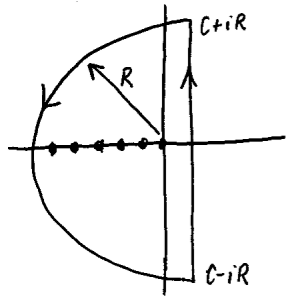
\includegraphics{figuras/15-0.jpg}
  \end{figure}
  Então
  \begin{dmath*}
    f(x) = \frac{1}{2 \pi i} \int_{C - i \infty}^{C + i \infty} x^{-p}
    \frac{\Gamma(p)}{\alpha p} \vi{p}
    = \frac{1}{2 \pi i} \int_{C - i \infty}^{C + i \infty} (\alpha x)^{-p}
    \Gamma(p) \vi{p}
    = \sum_{k = 0}^{\infty} \Res_{p = -k}\left[ (\alpha x)^{-p} \Gamma(p)
    \right].
  \end{dmath*}
  Em relação ao resíduo,
  \begin{dmath*}
    \Res_{p = -k}\left[ (\alpha x)^{-p} \Gamma(p) \right] = \lim_{p \to -k} (p +
    k) (\alpha x)^{-p} \Gamma(p)
    = \left[ \lim_{p \to -k} (p + k) \Gamma(p) \right] (\alpha x)^k.
  \end{dmath*}
  Mas $\Gamma(p + 1) = p \Gamma(p)$, de modo que
  \begin{dmath*}
    (p + k) \Gamma(p) = \frac{(p + k)}{p} \Gamma(p + 1)
    = \frac{(p + k)}{p (p + 1)} \Gamma(p + 2)
    = \ldots
    = \frac{(p + k) \Gamma(p + k + 1)}{p (p + 1) \ldots (p + k - 1) (p + k)}
    = \frac{\Gamma(p + k + 1)}{p (p + 1) \ldots (p + k - 1)}.
  \end{dmath*}
  Logo,
  \begin{dmath*}
    \lim_{p \to -k} (p + k) \Gamma(p) = \frac{\Gamma(1)}{(-k) (-k + 1) \ldots
    (-1)}
    = \frac{(-1)^{k} \Gamma(1)}{k (k - 1) \ldots 1}
    = \frac{(-1)^k}{k!}.
  \end{dmath*}
  E por fim,
  \begin{dmath*}
    f(x) = \sum_{k = 0}^{\infty} \frac{(-1)^k}{k!} (\alpha x)^k
    = \exp(-\alpha x).
  \end{dmath*}
\end{exem}

\begin{exem}
  Considere a função $f(x) = 1 / (1 + x)$. Para calcular
  \begin{dmath*}
    F(p) = \int_{0}^{\infty} \frac{x^{p - 1}}{1 + x} \vi{x}
  \end{dmath*}
  vamos considerar a integral no plano complexo:
  \begin{figure}[htb]
    \centering
    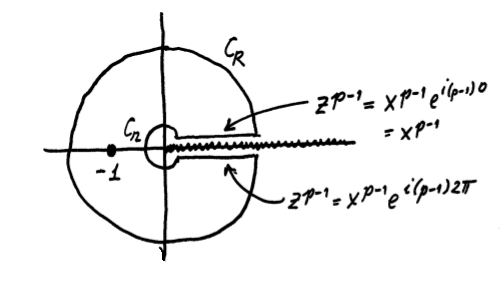
\includegraphics{figuras/15-1.jpg}
  \end{figure}
  \begin{dmath*}
    I(p) = \oint_C \frac{z^{p - 1}}{1 + z} \vi{z}.
  \end{dmath*}
  Como
  \begin{dmath*}
    z^{p - 1} = \exp\left( (p - 1) \ln z \right)
    = \exp\left( (p - 1) \left( \ln |z| + i (\theta + 2 \kappa \pi) \right) \right)
    = |z|^{p - 1} \exp\left( i (p - 1) (\theta + 2 k \pi \right).
  \end{dmath*}
  Podemos ainda notar que
  \begin{dgroup*}
    \begin{dmath*}
      \left| \int_{C_R} \left( \ldots \right) \right| \leq \int_0^{\infty}
      \frac{|r|^{p - 1} R}{R} \vi{\theta}
      \approx |R|^{p - 1}
      % TODO Quebrar linha aqui.
      \overset{R \to \infty}{\longrightarrow} 0 \condition{$p < 1$},
    \end{dmath*}
    \begin{dmath*}
      \left| \int_{C_R} \left( \ldots \right) \right| \leq \int_0^{\infty}
      \frac{|r|^{p - 1} r}{1 + r} \vi{r}
      \approx \int_0^{\infty} \frac{|r|^{p - 1} r}{r} \vi{r}
      \approx |r|^{-p}
      % TODO Quebrar linha aqui.
      \overset{R \to 0}{\longrightarrow} 0 \condition{$p > 0$}.
    \end{dmath*}
  \end{dgroup*}
  Então
  \begin{dmath*}
    2 \pi i \Res_{z = -1} f(z) = \int_r^R (\ldots) + \int_{C_R} (\ldots) +
    \int_R^r (\ldots) + \int_{C_R} (\ldots)
    = \lim_{r \to 0, R \to \infty} (\ldots)
    = \int_0^{\infty} (\ldots) + \int_{\infty}^0 (\ldots)
    = \int_0^{\infty} \frac{x^{p - 1}}{1 + x} \vi{x} + \int_{\infty}^0
    \frac{x^{p - 1} \exp(i (p - 1) 2 \pi)}{1 + x} \vi{x}
    = \left( 1 - \exp\left( i (p - 1) 2 \pi \right) \right) \int_0^{\infty}
    \frac{x^{p - 1}}{1 + x} \vi{x}
    = \exp\left( i (p - 1) \pi \right) \left( \exp\left( -i (p - 1) \pi \right)
    - \exp\left( i (p - 1) \pi \right)\right) \int_0^{\infty}
    \frac{x^{p - 1}}{1 + x} \vi{x}
    = \exp\left( i (p - 1) \pi \right) \left( -\exp\left( -i p \pi \right)
    + \exp\left( i p \pi \right)\right) \int_0^{\infty}
    \frac{x^{p - 1}}{1 + x} \vi{x}.
  \end{dmath*}
  Mas
  \begin{dmath*}
    \Res_{z = -1} f(z) = \lim_{z \to -1} (z + 1) \frac{z^{p - 1}}{1 + z}
    = (-1)^{p - 1}
    = \exp(i (p - 1) \pi)
  \end{dmath*}
  e, portanto,
  \begin{dmath*}
    2 \pi i \exp\left( i (p - 1) \pi \right) = e^{i (p - 1)} \left( \exp(i p
    \pi) - \exp(- i p \pi) \right) \int_0^{\infty} \frac{x^{p - 1}}{1 + x}
    \vi{x}.
  \end{dmath*}
  Conclui-se então que
  \begin{dmath*}
    \int_0^{\infty} \frac{x^{p - 1}}{1 + x} \vi{x} = F(p)
    = \pi / \sin(p \pi).
  \end{dmath*}

  Já para a transformada inversa:
  \begin{dmath*}
    f(x) = \frac{1}{2 \pi i} \int_{C - i \infty}^{C + i \infty}
    \frac{\pi}{\sin(p \pi)} x^{-p} \vi{p}
  \end{dmath*}
  onde os pólos simples em $p = k \pi$ para $k \in \mathbb{Z}$.
  \begin{figure}[htb]
    \centering
    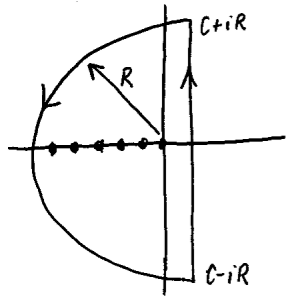
\includegraphics{figuras/15-0.jpg}
  \end{figure}
  Então, se $0 < x < 1$,
  \begin{dmath*}
    f(x) = \sum_{k = 0}^{\infty} \Res_{p = - k} \left[ \frac{\pi x^{-p}}{\sin(p
    \pi)} \right]
    = \sum_{k = 0}^{\infty} \lim_{p \to -k} (p + k) \frac{\pi}{\sin(p \pi)}
    x^{-p}
    = \sum_{k = 0}^{\infty} \lim_{q \to 0} \frac{q \pi x^{-(q - k)}}{\sin\left(
    (q - k) \pi \right)}
    = \sum_{k = 0}^{\infty} \lim_{q \to 0} \frac{q \pi x^{-(q - k)}}{(-1)^k
    \sin(q \pi)}
    = \sum_{k = 0}^{\infty} \lim_{q \to 0} \frac{q \pi}{\sin(q \pi)} x^{-q}
    \frac{x^k}{(-1)^k}
    = \sum_{k = 0}^{\infty} (-x)^k
    = 1 / \left( 1 - (-x) \right)
    = 1 / (1 + x),
  \end{dmath*}
  se $x > 1$,
  \begin{dmath*}
    f(x) = - \sum_{k = 1}^{\infty} \Res_{p = k} \left[ \frac{\pi x^{-p}}{\sin(p
    \pi)} \right]
    = - \sum_{k = 1}^{\infty} \lim_{p \to k} \frac{(p - k) \pi x^{-p}}{\sin(p
    \pi)}
    = - \sum_{k = 1}^{\infty} \lim_{q \to 0} \frac{q \pi x^{- (1 +
    k)}}{\sin\left( (q + k) \pi \right)}
    = - \sum_{k = 1}^{\infty} \lim_{q \to 0} \frac{q \pi x^{- (1 +
    k)}}{(-1)^k \sin(q \pi)}
    = - \sum_{k = 1}^{\infty} \lim_{q \to 0} \frac{q \pi}{\sin(q \pi)} x^{-q}
    \frac{x^{-k}}{(-1)^k}
    = - \sum_{k = 1}^{\infty} (-x^{-q})^k
    = - \left[ \sum_{k = 0}^{\infty} (-x^{-1})^k - 1 \right]
    = - \left[ \frac{1}{1 + x^{-1}} - 1 \right]
    = - \left[ \frac{1 - 1 - x^{-1}}{1 + x^{-1}} \right]
    = x^{-1} / \left( 1 + x^{-1} \right)
    = 1 / \left( x + 1 \right),
  \end{dmath*}
  e se $x = 1$,
  \begin{dmath*}
    f(1) = \frac{1}{2 \pi i} \int_{-i \infty}^{+i \infty} \frac{\pi}{\sin(p
    \pi)} \vi{p}
    = \frac{1}{2 \pi i} \lim_{R \to \infty} \int_{-i R}^{+i R}
    \frac{1}{\sin(p \pi)} \vi{(p \pi)}
    = \frac{1}{2 \pi i} \lim_{R \to \infty} \left. \left[ \ln \tan(p \pi / 2)
    \right] \right|_{-i R}^{+i R}
    = \frac{1}{2 \pi i} \lim_{R \to \infty} \left[ \ln \tan(i R \pi / 2) - \ln
    \tan(-i R \pi / 2) \right]
    = \frac{1}{2 \pi i} \lim_{R \to \infty} \ln \left[ \frac{\tan(i R \pi /
    2)}{\tan(- i R \pi / 2)} \right]
    = \frac{1}{2 \pi i} \lim_{R \to \infty} \ln \left[ \frac{\tan(i R \pi /
    2)}{- \tan(i R \pi / 2)} \right]
    = \frac{1}{2 \pi i} \ln(-1)
    = \frac{1}{2 \pi i} \ln\left( \exp(i \pi) \right)
    = \frac{1}{2 \pi i} i \pi
    = 1/2
  \end{dmath*}

  Conclusão, $f(x) = 1 / (1 + x)$.
\end{exem}

Para estudar algumas propriedades da transformada de Mellin, vamos usar uma
notação apropriada:
\begin{dmath*}
  \mathcal{M}[f](p) = \int_0^{\infty} f(x) x^{p - 1} \vi{x}.
\end{dmath*}

Algumas das propriedades mais importantes das transformadas de Mellin são:
\begin{dgroup*}
  \begin{dmath*}
    \mathcal{M}[x^{\alpha} f(x)](p) = \mathcal{M}[f(x)](p + \alpha),
  \end{dmath*}
  \begin{dmath*}
    \mathcal{M}[f'(x)](p) = -(p - 1) \mathcal{M}[f(x)](p - 1),
  \end{dmath*}
  \begin{dmath*}
    M[x f'(x)](p) = -p \mathcal{M}[f(x)](p),
  \end{dmath*}
  \begin{dmath*}
    M[x^n f^{(n)}(x)](p) = (-1)^n (p)_n \mathcal{M}[f(x)](p),
  \end{dmath*}
\end{dgroup*}
onde usamos o símbolo de Pochhammer, $(p)_n = p (p + 1) \ldots (p + n - 1)$.
Quanto à demonstração, a da primeira é óvia. Já a segunda se faz por partes,
sendo que observamos que devemos supor $\lim_{x \to 0} f(x) x^{p - 1} = 0$ para
$\Re(p) > \alpha$ e $\lim_{x \to \infty} f(x) x^{p - 1} = 0$ para $\Re(p) <
\beta$, sendo que $\mathcal{M}[f(x)](p)$ existe para $\alpha < \Re(p) < \beta$.
A terceira e a quarta sequem usando essas duas primeiras propriedades.

Quanto à propriedades de convolução, precisamos adaptar a sua definição para a
transformada de Mellin. Como passamos de Fourier para Mellin através da mudança
de variável $x = \exp(t)$, vamos fazer essa mudança na definição da convolução
dentro do contexto das transformadas de Fourier. Tomando $x = \exp(t)$ e
$\epsilon = \exp(\tau)$ temos
\begin{dmath*}
  \int_{-\infty}^{+\infty} f(\tau) g(t - \tau) \vi{\tau} = \int_0^{\infty} f(\ln
  \epsilon) g(\ln x - \ln \epsilon) (1 / \epsilon) \vi{\epsilon}
  = \int_0^{\infty} \epsilon^{-1} F(\epsilon) G(x / \epsilon) \vi{\epsilon}.
\end{dmath*}

Portanto, dentro do contexo das transformadas de Mellin, definimos a convolução
como
\begin{dmath*}
  (f * g)(x) = \int_0^{\infty} \epsilon^{-1} f(\epsilon) g(x / \epsilon)
  \vi{\epsilon}.
\end{dmath*}
Agora:
\begin{dmath*}
  \mathcal{M}[(f * g)(x)] = \int_0^{\infty} x^{p - 1} \int_0^{\infty}
  \epsilon^{-1} f(\epsilon) g(x / \epsilon) \vi{\epsilon} \vi{x}
  = \int_0^{\infty} \int_0^{\infty} x^{p - 1} \epsilon^{-1} f(\epsilon) g(x /
  \epsilon) \vi{\epsilon} \vi{x}
  = \int_0^{\infty} \int_0^{\infty} \epsilon (\epsilon y)^{p - 1} \epsilon^{-1}
  f(\epsilon) g(y) \vi{\epsilon} \vi{y}
  = \int_0^{\infty} y^{p - 1} g(y) \int_0^{\infty} \epsilon^{p - 1} f(\epsilon)
  \vi{\epsilon} \vi{y}
  = \mathcal{M}[f](p) \mathcal{M}[g](p)
\end{dmath*}
de modo que, com essa definição de convolução, temos
\begin{dmath*}
  \mathcal{M}[(f * g)(x)](p) = \mathcal{M}[f(x)](p) \mathcal{M}[g(x)](x).
\end{dmath*}

Outra propriedade a considerar envolve a transformada $\mathcal{M}[f(x \exp(i
\theta))]$. Temos
\begin{dmath*}
  \mathcal{M}[f(x \exp(i \theta))](p) = \int_0^{\infty} x^{p - 1} f(x \exp(i
  \theta)) \vi{x}
  = \exp(- i \theta p) \int_C y^{p - 1} f(y) \vi{y},
\end{dmath*}
onde tomamos $y = x \exp(i \theta)$. Visto que a operação $z \to z \exp(i
\theta)$ é uma rotação por um ângulo $\theta$ no plano complexo, o caminho $C$ é
o limite do caminho $C_R$ abaixo para $R \to \infty$. Se $f(y)$ é analítica na
região limitada pelas curvas abaixo, temos
\begin{figure}[htb]
  \centering
  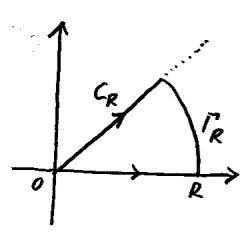
\includegraphics{figuras/15-3.jpg}
\end{figure}
\begin{dmath*}
  \oint = 0 \hiderel{=} - \int_{C_R} + \int_0^R + \int_{\Gamma_R}.
\end{dmath*}
Em $\Gamma_R$ temos $y = R \exp(i \theta)$, $\vi{y} = R \exp(i \theta) i
\vi{\theta}$ e
\begin{dmath*}
  \int_{\Gamma_R} R \exp(i \theta) \left( R \exp(i \theta) \right)^{p - 1}
  f\left( R \exp(i \theta) \right) i \vi{\theta} = \int_{\Gamma_R} \exp(i \theta
  p) R^p f(R \exp(i \theta) i \vi{\theta},
\end{dmath*}
ou seja,
\begin{dmath*}
  \int_{\Gamma_R} \overset{R \to \infty}{\longrightarrow} 0 \condition{se $R^p
  f(R) \overset{R \to \infty}{\longrightarrow} 0$}.
\end{dmath*}
Com essa hipótese, temos $\int_C = \int_0^{\infty}$ e portanto
\begin{dmath*}
  \mathcal{M}[f(x \exp(i \theta))](p) = \exp(-i \theta p) \mathcal{M}[f(x)](p)
\end{dmath*}
ou ainda
\begin{dgroup*}
  \begin{dmath*}
    cos(\theta p) \mathcal{M}[f(x)](p) = \Re[\mathcal{M}[f(x \exp(i \theta))]](p)
  \end{dmath*}
  \begin{dmath*}
    \sin(\theta p) \mathcal{M}[f(x)](p) = -\Im[\mathcal{M}[f(x \exp(i \theta))]](p).
  \end{dmath*}
\end{dgroup*}

\begin{exem}
  Já vimos que
  \begin{dmath*}
    \mathcal{M}[1 / (1 + x)] = \pi / \sin(p \pi).
  \end{dmath*}
  Agora vamos verificar que
  \begin{dmath*}
    \mathcal{M}[H(Q - x)] = \int_0^{\infty} x^{p - 1} H(a - x) \vi{x}
    = \int_0^{\alpha} x^{p - 1} \vi{x}
    = a^p / p \condition{$p > 0$}.
  \end{dmath*}
  Então temos a convolução:
  \begin{dmath*}
    \int_0^{\infty} \epsilon^{-1} H(a - \epsilon) \frac{1}{1 + x / \epsilon}
    \vi{\epsilon} = \int_0^a \epsilon^{-1} \frac{\epsilon}{\epsilon + x}
    \vi{\epsilon}
    = \left. \ln(\epsilon + x) \right|_0^a
    = \ln\left( (x + a) / x \right).
  \end{dmath*}
  Portanto,
  \begin{dmath*}
    \mathcal{M}[\ln(1 + a / x)] = \frac{a^p}{p} \frac{\pi}{\sin(p \pi)}.
  \end{dmath*}
\end{exem}

\begin{exem}
  Considere
  \begin{dmath*}
    \mathcal{M}[1 / (1 + x^a)] = \int_0^{\infty} \frac{x^{p - 1}}{1 + x^a}
    \vi{x}
    = \frac{1}{a} \int_0^{\infty} \frac{y^{p / a - 1}}{1 + y} \vi{y}
    = \frac{1}{a} \frac{\pi}{\sin(p \pi / a)}.
  \end{dmath*}
  Então
  \begin{dmath*}
    \mathcal{M}[f(x \exp(i \theta))] = \int_0^{\infty} \frac{x^{p - 1}}{1 + (x
    (\exp(i \theta))^a} \vi{x}
    = \int_0^{\infty} \frac{x^{p - 1}}{1 + x^a \exp(i \theta a)} \vi{x}
    = \int_0^{\infty} \frac{x^{p - 1}}{1 + x^a \cos(\theta a) + i x^a
    \sin(\theta a)} \vi{x}
    = \int_0^{\infty} \frac{x^{p - 1} (1 + x^a \cos(\theta a) - i x^a
    \sin(\theta a)}{(1 + x^a \cos(\theta a))^2 + (x^a \sin(\theta a))^2}
    = \int_0^{\infty} \frac{x^{p - 1}(1 + x^a \cos(\theta a) - i x^a \sin(\theta
    a)}{1 + 2 x^a \cos(\theta a) + x^{2 a}} \vi{x}
    = \exp(-i p \theta) \int_0^{\infty} \frac{x^{p - 1}}{1 + x^a} \vi{x}
    = \exp(-i p \theta) \frac{\pi}{a \sin(p \pi / a)}.
  \end{dmath*}
  Logo,
  \begin{dgroup*}
    \begin{dmath*}
      \cos(\theta p) \frac{\pi}{a \sin(p \pi /a} = \mathcal{M}\left[ \frac{1 +
      x^a \cos(\theta a)}{1 + 2 x^a \cos(\theta a) + x^{2 a}} \right]
    \end{dmath*}
    \begin{dmath*}
      \sin(\theta p) \frac{\pi}{a \sin(p \pi / a)} = \mathcal{M}\left[ \frac{x^a
      \sin(\theta a)}{1 + 2 x^a \cos(\theta a) + x^{2 a}} \right]
    \end{dmath*}
  \end{dgroup*}
\end{exem}

% TODO Adicionar o exemplo que inicia-se na página 2 de M2S12-16.pdf

\section{Transformada de Hankel}
Vamos considerar uma função de duas variáveis $f(x, y)$ e a sua transformada de
Fourier $F(K, L)$, ou seja,
\begin{dgroup*}
  \begin{dmath*}
    F(K, L) = \frac{1}{2 \pi} \int_{-\infty}^{+\infty} \int_{-\infty}^{+\infty}
    f(x, y) \exp\left( i (K x + L y) \right) \vi{y} \vi{x},
  \end{dmath*}
  \begin{dmath*}
    f(x, y) = \frac{1}{2 \pi} \int_{-\infty}^{+\infty} F(K, L) \exp\left( i (K x
    + L y) \right) \vi{L} \vi{K}.
  \end{dmath*}
\end{dgroup*}
Agora vamos passar apra coordenadas polares. Por abuso de notação, vamos denotar
$f(r, \theta) = f(x(r, \theta), y(r, \theta))$ e $F(\rho, \varphi) = F(K(\rho,
\varphi), L(\rho, \varphi))$. Uma vez que essas funções tem periodicidade
angular, ou seja, temos $f(r, \theta + 2 \pi) = f(r, \theta)$ e $F(\pi, \varphi
+ 2 \pi) = F(\rho, \varphi)$, podemos nessa variável tomar uma séria de Fourier,
de modo que
\begin{dgroup*}
  \begin{dmath}
    f(r, \theta) = \sum_{n = -\infty}^{+\infty} f_n(r) \exp(i n \theta),
  \end{dmath}
  \begin{dmath*}
    f_n(r) = \frac{1}{2 \pi} \int_0^{2 \pi} f(r, \theta) \exp(-i n \theta)
    \vi{\theta},
  \end{dmath*}
  \begin{dmath*}
    F(\rho, \varphi) = \sum_{n = -\infty}^{+\infty} F_n(\rho) \exp(i n \varphi),
  \end{dmath*}
  \begin{dmath*}
    F_n(\rho) = \frac{1}{2 \pi} \int_0^{2 \pi} F(\rho, \varphi) \exp(-i n
    \varphi) \vi{\varphi}.
  \end{dmath*}
\end{dgroup*}
Em coordenadas polares temos
\begin{dmath*}
  F(\rho, \varphi) = \frac{1}{2 \pi} \int_0^{\infty} r \int_0^{2 \pi} f(r,
  \theta) \exp\left(i \left[ (\rho \cos\varphi) (r \cos\theta) + (\rho \sin\varphi)
  (r \sin\theta) \right] \right) \vi{\theta} \vi{r}
  = \frac{1}{2 \pi} \int_0^{\infty} r \int_0^{2 \pi} f(r, \theta) \exp(i p r
  \cos(\varphi - \theta)) \vi{\theta} \vi{r}
\end{dmath*}
e portanto
\begin{dmath*}
  F_n(\rho) = \frac{1}{2 \pi} \int_0^{2 \pi} \exp(-i n \varphi)
  \frac{1}{2 \pi} \int_0^{\infty} r \int_0^{2 \pi} f(r, \theta) \exp(i \rho r
  \cos(\varphi - \theta)) \vi{\theta} \vi{r} \vi{\varphi}
  = \frac{1}{(2 \pi)^2} \int_0^{\infty} r \int_0^{2 \pi} \int_0^{2 \pi} \exp(-i
  n \varphi) \exp(i \rho r \cos(\varphi - \theta)) \sum_{m = -\infty}^{+\infty}
  f_m(r) \exp(i m \theta) \vi{\theta} \vi{\varphi} \vi{r}
  = \frac{1}{(2 \pi)^2} \int_0^{\infty} r \sum_{m = -\infty}^{+\infty} f_m(r)
  \int_0^{2 \pi} \int_0^{2 \pi} \exp(-i n (\alpha + \theta)) \exp(i \rho r
  \cos(\alpha)) \exp(i m \theta) \vi{\theta} \vi{\alpha} \vi{r}
\end{dmath*}
onde usamos, na integração em $\alpha$, o fato da periodicidade ser $2 \pi$, o
que implica que $\int_{0 + \theta}^{2 \pi + \theta} (\ldots) \vi{\alpha} =
\int_0^{2 \pi} (\ldots) \vi{\alpha}$. Continuando:
\begin{dmath*}
  F_n(\rho) = \frac{1}{2 \pi} \int_0^{\infty} r \sum_{m = -\infty}^{+\infty}
  f_m(r) \int_0^{2 \pi} \exp(-i n \alpha) \exp(i p r \cos\alpha)
  \frac{1}{2 \pi} \int_0^{2 \pi} \exp(-i n \theta) \exp(i m \theta) \vi{\theta}
  \vi{\alpha} \vi{r}
  = \frac{1}{2 \pi} \int_0^{\infty} r \sum_{m = -\infty}^{+\infty}
  f_m(r) \int_0^{2 \pi} \exp(-i n \alpha) \exp(i p r \cos\alpha)
  \sigma_{mn} \vi{\alpha} \vi{r}
  = \frac{1}{2 \pi} \int_0^{\infty} r f_n(r) \int_0^{2 \pi} \exp(-i r \alpha)
  \exp(i \rho r \cos\alpha) \vi{\alpha} \vi{r}.
\end{dmath*}
Mas a função geratriz para as funções de Bessel é
\begin{dmath*}
  \exp\left( z (t - 1/t) / 2 \right) = \sum_{n = -\infty}^{+\infty} t^n J_n(z),
\end{dmath*}
ou, tomando $t = i \exp(i \varphi)$
\begin{dmath*}
  \exp(i z \cos\varphi) = \sum_{n = -\infty}^{+\infty} i^n \exp(i n \varphi)
  J_n(z)
\end{dmath*}
de modo que
\begin{dmath*}
  \frac{1}{2 \pi} \int_0^{2 \pi} \exp(-i n \varphi) \exp(i z \cos\varphi) = i^n
  J_n(z)
\end{dmath*}
e portanto
\begin{dmath*}
  F_n(\rho) = \int_0^{\infty} r f_n(r) i^n J_n(\rho r) \vi{r}.
\end{dmath*}
De modo análogo:
\begin{dmath*}
  f_n(r) = \frac{1}{2 \pi} \int_0^{2 \pi} \exp(-i n \theta)
  \frac{1}{2 \pi} \int_0^{\infty} \rho \int_0^{2 \pi} F(\rho, \varphi) \exp\left(-i
  \rho r \cos(\theta - \varphi) \right) \vi{\varphi} \vi{\rho} \vi{\theta}
  = \frac{1}{2 \pi} \int_0^{\infty} \rho \int_0^{2 \pi} \exp(-i n \alpha)
  \exp(-i \rho r \cos\alpha) \sum_{m = -\infty}^{+\infty} F_m(\rho)
  \frac{1}{2 \pi} \int_0^{2 \pi} \exp(-i n \varphi) \exp(i m \varphi)
  \vi{\varphi} \vi{\alpha} \vi{\rho}
  = \frac{1}{2 \pi} \int_0^{\infty} \rho \int_0^{2 \pi} \exp(-i n \alpha)
  \exp(-i \rho r \cos\alpha) \sum_{m = -\infty}^{+\infty} F_m(\rho)
  \sigma_{mn} \vi{\alpha} \vi{\rho}
  = \int_0^{\infty} \rho F_n(\rho) \frac{1}{2 \pi} \int_0^{2 \pi} \exp(-i r
  \alpha) \exp(-i \rho r \cos\alpha) \vi{\alpha} \vi{\rho}
  = \int_0^{\infty} \rho F_n(\rho) (-i)^n J_n(\rho r) \vi{\rho}.
\end{dmath*}
Resumindo, temos:
\begin{dgroup*}
  \begin{dmath*}
    F_n(\rho) = i^n \int_0^{\infty} r J_n(\rho r) f_n(r) \vi{r},
  \end{dmath*}
  \begin{dmath*}
    f_n(r) = (-i)^n \int_0^{\infty} \rho J_n(\rho r) F_n(\rho) \vi{\rho},
  \end{dmath*}
\end{dgroup*}
o que nos sugere definir a transformada de Hankel de ordem $\nu$,
$\mathcal{H}_{\nu}$, e sua inversa, $\mathcal{H}_{\nu}^{-1}$ como
\begin{dgroup*}
  \begin{dmath*}
    \mathcal{H}_{\nu}[f(x)] = \int_0^{\infty} x J_{\nu}(K x) f(x) \vi{x}
    \hiderel{=} F_{\nu}(K),
  \end{dmath*}
  \begin{dmath*}
    \mathcal{H}_{\nu}^{-1}[F_{\nu}(K)] = \int_0^{\infty} K J_{\nu}(K x)
    F_{\nu}(K) \vi{K} \hiderel{=} f(x).
  \end{dmath*}
\end{dgroup*}

\begin{exem}
  Vamos calcular $\mathcal{H}_0[\exp(-\alpha x)]$.
  \begin{dmath*}
    \mathcal{H}[\exp(-\alpha x)] = \int_0^{\infty} x J_0(K x) \exp(-\alpha x)
    \vi{x}
    = \sum_{n = 0}^{\infty} \frac{(-1)^n K^{2n}}{2^{2n} (n!)^2} \int_0^{\infty}
    x^{2 n + 1} \exp(-\alpha x) \vi{x}
    = \sum_{n = 0}^{\infty} \frac{(-1)^n K^{2 n}}{2^{2 n} (n!)^2}
    \frac{\Gamma(2 n + 2)}{a^{2 n + 2}}
  \end{dmath*}
  mas da fórmula de duplicação de Legendre,
  \begin{dmath*}
    \sqrt{\pi} \Gamma(2 z + 1) = 2^{2 z} \Gamma(z + 1 / z) \Gamma(z + 1),
  \end{dmath*}
  temos
  \begin{dmath*}
    \Gamma(2 n + 1) = \Gamma\left[ 2 (n + 1 / 2) + 1 \right]
    = \frac{2^{2 (n + 1 / 2)}}{\sqrt{\pi}} \Gamma\left[ 1 + (1/2) + (1/2)
    \right] \Gamma\left[ n + (1/2) + 1 \right]
  \end{dmath*}
  e portanto
  \begin{dmath*}
    \mathcal{H}_0[\exp(-\alpha x)] = \sum_{K = 0}^{\infty} \frac{(-1)^n K^{2
    n}}{2^{2 n} [\Gamma(n + 1)]^2} \frac{2^{2 n} 2}{\sqrt{\pi}}
    \frac{\Gamma(n + 1) \Gamma(n + 3 / 2}{\alpha^{2 n + 2}}
    = \frac{1}{\alpha^2} \sum_{n = 0}^{\infty} \frac{(-1)^n (K / \alpha)^{2
    n}}{\Gamma(n + 1)} \frac{\Gamma(n + 3/2)}{\Gamma(3/2)}
    = \frac{1}{a^2} \sum_{n = 0}^{\infty} \frac{(-1)^n (K / \alpha)^{2
    n}}{\Gamma(n + 1)} \frac{\Gamma(n + 3/2)}{\sqrt{\pi} / 2}
    = \frac{1}{\alpha^2} \sum_{n = 0}^{\infty} (-1)^n (3/2)_n
    \frac{[(k/\alpha)^2]^n}{n!}
    = \frac{1}{\alpha^2} \frac{1}{[1 + (x / \alpha)^2]^{3/2}}
    = \frac{a}{(\alpha^2 + x^2)^{3/2}}.
  \end{dmath*}
\end{exem}

Uma das propriedades que mais nos interessa no caso de uma transformada integral
envolve a derivada de uma função. Nesse caso temos
\begin{dmath*}
  \mathcal{H}_{\nu}[f'(x)] = \int_0^{\infty} x J_{\nu}(K x) f'(x) \vi{x}
  = \left. x J_{\nu}(K x) f(x) \right|_0^{\infty} - \int_0^{\infty} \left[ x
  J_{\nu}(K x) \right]' f(x) \vi{x}
  = - \int_0^{\infty} \left[ x J_{\nu}(K x) \right]' f(x) \vi{x} \condition{se
  $\lim_{x \to \infty} f(x) = 0$.}
\end{dmath*}
Sabemos, porém, que
\begin{dgroup*}
  \begin{dmath*}
    2 J_{\nu}'(x) = J_{\nu - 1}(x) - J_{\nu + 1}(x),
  \end{dmath*}
  \begin{dmath*}
    \nu J_{\nu}(x) = \frac{x}{2} J_{\nu + 1}(x) + \frac{x}{2} J_{\nu - 1}(x)
  \end{dmath*}
\end{dgroup*}
Logo:
\begin{dmath*}
  (x J_{\nu}(x))' = J_{\nu}(x) + x J_{\nu}'(x)
  = \frac{x}{2 \nu} \left( J_{\nu + 1}(x) + J_{\nu - 1}(x) \right) +
  \frac{x}{2} \left( J_{\nu - 1}(x) - J_{\nu + 1}(x) \right)
  = \frac{x}{2} J_{\nu + 1}(x) \left( \frac{1 - \nu}{\nu} \right) +
  \frac{x}{2} J_{\nu - 1}(x) \left( \frac{1 + \nu}{\nu} \right).
\end{dmath*}
Sendo assim
\begin{dmath*}
  \mathcal{H}_{\nu}[f'(x)] = - K \int_0^{\infty} \left[ \frac{x}{2} J_{\nu +
  1}(K x) \left( \frac{1 - \nu}{\nu} \right) + \frac{x}{2} J_{\nu - 1}(K x)
  \left( \frac{1 + \nu}{\nu} \right) \right] f(x)
  = -K \left( \frac{1 - \nu}{2 \nu} \right) \mathcal{H}_{\nu + 1}[f(x)] - K
  \left( \frac{1 + \nu}{2 \nu} \right) \mathcal{H}_{\nu - 1}[f(x)]
  \condition{$\nu \geq 1$.}
\end{dmath*}
Não é, porém, nesse caso que a transformada de Hankel assume seu papel mais
simples. De fato, temos
\begin{dmath*}
  \mathcal{H}_{\nu}\left[ f''(x) + \frac{1}{x} f'(x) - \frac{\nu^2}{x^2} f(x)
  \right] = \int_0^{\infty} \left[ f''(x) + \frac{1}{x} f'(x) -
  \frac{\nu^2}{x^2} f(x) \right] J_{\nu}(K x) x \vi{x}
  = \left. f'(x) J_{\nu}(K x) x \right|_0^{\infty} + \left. f(x) J_{\nu}(K x)
  \right|_0^{\infty} + \int_0^{\infty} \left[ -f'(x) \left( J_{\nu}(K x) x
  \right)' - f(x) J_{\nu}' (K x) - \frac{\nu^2}{x} f(x) J_{\nu}(K x) \right]
  \vi{x}
  = \int_0^{\infty} \left[ -f'(x) \left( J_{\nu}(K x) x \right)' - f(x) J_{\nu}'
  (K x) - \frac{\nu^2}{x} f(x) J_{\nu}(K x) \right] \vi{x}
  = \left. -f(x) \left( J_{\nu}(K x) x \right)' \right|_0^{\infty} +
  \int_0^{\infty} \left[ f(x) \left( J_{\nu}(K x) x \right)'' - f(x) J_{\nu}'(K
  x) - \frac{\nu^2}{x} f(x) J_{\nu}(K x) \right] \vi{x}
  = \int_0^{\infty} \left[ f(x) \left( J_{\nu}(K x) x \right)'' - f(x) J_{\nu}'(K
  x) - \frac{\nu^2}{x} f(x) J_{\nu}(K x) \right] \vi{x}
  = \int_0^{\infty} \left[ f(x) \left( J_{\nu}'(K x) x + J_{\nu}(K x) \right)' -
  f(x) J_{\nu}'(K x) - \frac{\nu^2}{x} f(x) J_{\nu}(K x) \right] \vi{x}
  = \int_0^{\infty} \left[ f(x) \left( J_{\nu}''(K x) x + 2 J_{\nu}'(K x)
  \right) - f(x) J_{\nu}'(K x) - \frac{\nu^2}{x} f(x) J_{\nu}(K x) \right]
  \vi{x}
  = \int_0^{\infty} \left[ f(x) J_{\nu}''(K x) x + 2 f(x) J_{\nu}'(K x) - f(x)
  J_{\nu}'(K x) - \frac{\nu^2}{x} f(x) J_{\nu}(K x) \right] \vi{x}
  = \int_0^{\infty} f(x) x \left[ J_{\nu}''(K x) + (1 / x) J_{\nu}'(K x) -
  \frac{\nu^2}{x^2} J_{\nu}(K x) \right] \vi{x}
\end{dmath*}
mas, da equação de Bessel para $z = K x$, segue que
\begin{dmath*}
  J_{\nu}''(K x) + J_{\nu}'(K x) + \left( K^2 - \frac{\nu^2}{x^2} \right)
  J_{\nu}(K x) = 0
\end{dmath*}
e portanto
\begin{dmath*}
  \int_0^{\infty} f(x) x \left[ J_{\nu}''(K x) + (1 / x) J_{\nu}'(K x) -
  \frac{\nu^2}{x^2} J_{\nu}(K x) \right] \vi{x} = \int_0^{\infty} f(x) \left[
  -K^2 J_{\nu}(K x) \right] x \vi{x}
  = -K^2 \mathcal{H}_{\nu}[f(x)].
\end{dmath*}

% TODO Adicionar exemplo da página 11 de M2S12-16.pdf


\backmatter

\appendix
% Filename: licenca@notas_de_aula.tex
% This code is part of 'Notas de aula n\~{a}o oficiais de MS650 e F620'
% 
% Description: This file correspond to part of the textbook using in the course.
% 
% Created: 02.08.12 10:36:23 PM
% Last Change: 02.08.12 10:36:23 PM
% 
% Authors:
% - Raniere Silva, r.gaia.cs@gmail.com
% 
% Copyright (c) 2012, Raniere Silva. All rights reserved.
% 
% This work is licensed under the Creative Commons Attribution-NonCommercial-NoDerivs 3.0 Unported License. To view a copy of this license, visit http://creativecommons.org/licenses/by-nc-nd/3.0/.
%
% This work is distributed in the hope that it will be useful, but WITHOUT ANY WARRANTY; without even the implied warranty of MERCHANTABILITY or FITNESS FOR A PARTICULAR PURPOSE.
%
\chapter{Licen\c{c}a e Notas de Esclarecimento}
Este trabalho \'{e} baseado nos manuscritos das notas de aula do Professor Doutor Jayme Vaz Jr. para as disciplinas MS650, M\'{e}todos de Matem\'{a}tica Aplicada II, e F620, M\'{e}todos Matem\'{a}ticos da F\'{i}sica II, disponibilizadas em \url{http://www.ime.unicamp.br/~vaz/metodos2S12.htm}. \'{E} permitido a este fazer uso deste trabalho para qualquer fim e sem nenhuma restri\c{c}\~{a}o.

Salvo indica\c{c}\~{a}o em contr\'{a}rio, este trabalho foi licenciado com a Creative Commons Atribui\c{c}\~{a}o - N\~{a}oComercial - SemDerivados 3.0 N\~{a}o Adaptada. Para ver uma c\'{o}pia desta licen\c{c}a, visite \url{http://creativecommons.org/licenses/by-nc-nd/3.0/}.
%The photo X is © 2009 Jane Park, used under a Creative Commons Attribution-Noncommercial license: http://creativecommons.org/licenses/by-nc/3.0/.
\begin{center}
    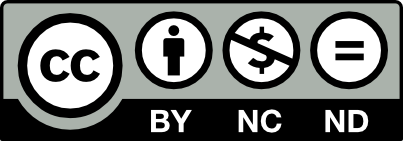
\includegraphics[keepaspectratio=true]{cc-by-nc-nd.png}
\end{center}

Este trabalho encontra-se dispon\'{i}vel em % Filename: repository.tex
% 
% This code is part of 'Solutions for MS550, M\'{e}todos de Matem\'{a}tica Aplicada I, and F520, M\'{e}todos Matem\'{a}ticos da F\'{i}sica I'
% 
% Description: This file keeps the url of the repository.
% 
% Created: 07.03.12 04:00:00 PM
% Last Change: 14.07.12 10:17:20 AM
% 
% Authors:
% - Raniere Silva (2012): initial version
% 
% Copyright (c) 2012 Raniere Silva <r.gaia.cs@gmail.com>
% 
% This work is licensed under the Creative Commons Attribution-ShareAlike 3.0 Unported License. To view a copy of this license, visit http://creativecommons.org/licenses/by-sa/3.0/ or send a letter to Creative Commons, 444 Castro Street, Suite 900, Mountain View, California, 94041, USA.
%
% This work is distributed in the hope that it will be useful, but WITHOUT ANY WARRANTY; without even the implied warranty of MERCHANTABILITY or FITNESS FOR A PARTICULAR PURPOSE.
%
\url{https://github.com/r-gaia-cs/solucoes_ms650_f620}
 e atualmente \'{e} mantido por % Filename: maintainer_name.tex
% 
% This code is part of 'Solutions for MS550, Métodos de Matemática Aplicada I, and F520, Métodos Matemáticos da F\'{i}sica I'
% 
% Description: This file keeps the email of the mainteiner.
% 
% Created: 02.08.12 10:41:35 PM
% Last Change: 02.08.12 10:41:35 PM
% 
% Authors:
% - Raniere Silva (2012): initial version
% 
% Copyright (c) 2012 Raniere Silva <r.gaia.cs@gmail.com>
% 
% This work is licensed under the Creative Commons Attribution-ShareAlike 3.0 Unported License. To view a copy of this license, visit http://creativecommons.org/licenses/by-sa/3.0/ or send a letter to Creative Commons, 444 Castro Street, Suite 900, Mountain View, California, 94041, USA.
%
% This work is distributed in the hope that it will be useful, but WITHOUT ANY WARRANTY; without even the implied warranty of MERCHANTABILITY or FITNESS FOR A PARTICULAR PURPOSE.
%
Raniere Silva
 (% Filename: maintainer.tex
% 
% This code is part of 'Solutions for MS550, Métodos de Matemática Aplicada I, and F520, Métodos Matemáticos da F\'{i}sica I'
% 
% Description: This file keeps the email of the mainteiner.
% 
% Created: 07.03.12 04:00:00 PM
% Last Change: 30.05.12 04:40:25 PM
% 
% Authors:
% - Raniere Silva (2012): initial version
% 
% Copyright (c) 2012 Raniere Silva <r.gaia.cs@gmail.com>
% 
% This work is licensed under the Creative Commons Attribution-ShareAlike 3.0 Unported License. To view a copy of this license, visit http://creativecommons.org/licenses/by-sa/3.0/ or send a letter to Creative Commons, 444 Castro Street, Suite 900, Mountain View, California, 94041, USA.
%
% This work is distributed in the hope that it will be useful, but WITHOUT ANY WARRANTY; without even the implied warranty of MERCHANTABILITY or FITNESS FOR A PARTICULAR PURPOSE.
%
\href{mailto:r.gaia.cs@gmail.com}{r.gaia.cs@gmail.com}
).

Este trabalho \'{e} distribuido na esperança que possa ser \'{u}til, mas SEM NENHUMA GARANTIA; sem uma garantia implicita de ADEQUA\c{C}\~{A}O a qualquer MERCADO ou APLICA\c{C}\~{A}O EM PARTICULAR.


% References
\nocite*
\bibliographystyle{alpha}
\bibliography{../bibliography}

% Show index.
\addcontentsline{toc}{chapter}{Index}
\printindex
\end{document}
